\NeedsTeXFormat{LaTeX2e}

\documentclass[a4paper,12pt]{pkg/monografia}
\usepackage[pdfpagelabels]{hyperref}
\usepackage{amsmath,amsthm,amsfonts,amssymb}
\usepackage[mathcal]{eucal}
\usepackage{latexsym}
%\usepackage[utf8]{inputenc}
\usepackage[brazil]{babel}
%\usepackage{bm}
\usepackage[alf]{pkg/abntex2cite}
\usepackage{url}
\usepackage{enumitem}
\usepackage{graphicx}
\usepackage{placeins}
%\usepackage{epstopdf}
\usepackage{multirow}
%\usepackage{fancyhdr}
\usepackage{textcase}
\usepackage{tabularx}
\usepackage[table,xcdraw]{xcolor}
%\usepackage[portuguese,noend,ruled]{algorithm2e}
\usepackage{listings}
\usepackage[T1]{fontenc}
\usepackage{courier}
\usepackage[printonlyused]{acronym}
\usepackage{caption}
\usepackage{adjustbox}
\usepackage{floatrow}
\floatsetup[figure]{capposition=top}
\floatsetup[table]{capposition=top}
%\captionsetup{labelsep=endash}
%\usepackage{rotating}
%\usepackage{rotfloat}
%\usepackage{placeins}
\usepackage{fontspec}
\setmonofont{Inconsolata}
%\captionsetup[listing]{position=top}
\usepackage{makecell}
\usepackage{listings}
\usepackage{epigraph}
\usepackage{subcaption}

%-----------------------------------------------------------
\begin{document}

%----------------- Título e Dados do Autor -----------------
\titulo{Análise de arquiteturas de microsserviços empregados a jogos MMORPG voltada a otimização do uso de recursos computacionais}
\autor{Marlon Henry Schweigert}
\nome{Marlon Henry}
\ultimonome{Schweigert}

%---------- Informe o Curso e Grau -------------------------
\bacharelado \curso{Ciência da Computação} \mes{Dezembro} \ano{2018}
\data{\today} % Data da aprovação
\cidade{Joinville}

%---------- Informações sobre a Institução -----------------
\instituicao{Universidade do Estado de Santa Catarina}
\sigla{UDESC} \unidadeacademica{Centro de Ciências Tecnológicas}

%-- Nomes do Orientador, 1o. Examinador e 2o. Examinador ---
\orientador{Charles Christian Miers}
\examinadorum{Débora Cabral Nazário}
\examinadordois{Guilherme Piêgas Koslovski}
%\examinadortres{}

%-- Títulos do Orientador, 1o. Examinador e 2o. Examinador -
\ttorientador{Doutor}
\ttexaminadorum{Doutora}
\ttexaminadordois{Doutor}
%\ttexaminadortres{}

%---------- Capa -------------------------------------------
\maketitle

%---------- Agradecimentos----------------------------------
%\agradecimento{Agradecimentos}
\section*{Agradecimentos}

AGRADECIMENTOS

\newpage

%---------- Epígrafe ---------------------------------------
\begin{epigrafe}
	\begin{flushright}
		\vspace*{\fill}
		\textit{``É um erro acreditar que é possível resolver qualquer problema importante usando batatas.``}\\
		(Douglas Adams)
		\par
	\end{flushright}
\end{epigrafe}
\newpage

%---------- Resumo -----------------------------------------
\resumo{Resumo}
A crescente popularização de jogos \acf{mmorpg} demanda por novas abordagens tecnológicas, a fim de suprir as necessidades dos usuários com menor custo de recursos computacionais.
%
Projetar essas arquiteturas, do ponto de vista da rede, é algo pertinente e impactante para o sucesso desses jogos.
%
O objetivo deste trabalho é propor uma análise voltada a identificar os recursos computacionais consumidos pelas arquiteturas identificadas.
%
Esse objetivo será atingido após realizar uma pesquisa referenciada, seguida de uma análise das principais arquiteturas e, preferencialmente, a execução de simulações de clientes usando as arquiteturas implantadas em uma nuvem computacional para auxiliar na identificação de gargalos de recursos. 
%
Os resultados obtidos auxiliarão provedores de serviços \ac{mmorpg} a reduzir gastos de manutenção e melhorar a qualidade de tais serviços.

\\
\noindent \textbf{Palavras-chaves:} Arquitetura de Microsserviços, Desenvolvimento de Jogos, Rede de Jogos,
Jogos Massivos, Otimização de Recursos, Nuvem de Computadores.

%---------- Abstract ---------------------------------------
\resumo{Abstract}
The increasing popularization of mass games demands new technological approaches in order to meet the needs of users with lower cost of computational resources.
%
Designing these architectures, from the network point of view, is relevant and impacting to the success of these games.
%
The objective of this work is to propose an analysis aimed at identifying approaches to optimize the computational resources consumed by the identified architectures.
%
This objective will be achieved after conducting a referenced search, followed by an analysis of the main architectures and, respectively, the execution of simulations using a computational cloud to assist in the identification of resource bottlenecks.
%
The results obtained will help \ac{mmorpg} service providers to reduce maintenance costs and improve the quality of such services.
\\
\noindent \textbf{Keywords:} Microservice Architecture, Game Development, Game Network, Massive Games, Resource Optimization, Cloud Computing.

%-----------------------------------------------------------

% SUMÁRIO, LISTA DE FIGURAS E LISTA DE TABELAS
%---------- Sumário ----------------------------------------
\tableofcontents
\thispagestyle{empty}

%---------- Lista de figuras -------------------------------
\listoffigures
\thispagestyle{empty}

%---------- Lista de tabelas -------------------------------
\listoftables
\thispagestyle{empty}

%---------- Lista de Abreviaturas --------------------------
\listofabbreviations{Lista de Abreviaturas}
\begin{acronym}[]
	\acro{amqp}[AMQP]{{\it Advanced Message Queuing Protocol}}
	\acro{api}[API]{{\it Application Programming Interface}}
    \acro{aws}[AWS]{{\it Amazon Web Services}}
	\acro{cli}[CLI]{{\it Command Line Interface}}
	\acro{ddos}[DDoS]{{\it Distributed Denial of Service}}
	\acro{iaas}[IaaS]{{\it Infrastructure as a Service}}
    \acro{ids}[IDS]{{\it Intrusion Detection System}}
	\acro{kvm}[KVM]{{\it Kernel-based Virtual Machine}}
    \acro{ldap}[LDAP]{{\it Lightweight Directory Access Protocol}}
	\acro{nist}[NIST]{{\it National Institute of Standards and Technology}}
	\acro{paas}[PaaS]{{\it Platform as a Service}}
    \acro{rpc}[RPC]{{\it Remote Procedure Call}}
	\acro{saas}[SaaS]{{\it Software as a Service}}
	\acro{snmp}[SNMP]{{\it Simple Network Management Protocol}}
	\acro{qos}[QoS]{{\it Quality of Service}}
	\acro{sdn}[SDN]{{\it Software Defined Network}}
	\acro{vlan}[VLAN]{{\it Virtual Local Area Network}}
	\acro{vm}[VM]{{\it Virtual Machine}}
	\acro{vpn}[VPN]{{\it Virtual Private Network}}

	\acro{POV}[POF]{{\it Point of View}}

	\acro{FPS}[FPS]{{\it First-person shooter}}
	\acro{TPS}[TPS]{{\it Third-person shooter}}
	\acro{RTS}[RTS]{{\it Real-time strategy}}
	\acro{MMO}[MMO]{{\it Massively multiplayer online}}
	\acro{RPG}[RPG]{{\it Role-playing game}}
	\acro{MMORPG}[MMORPG]{{\it Massively multiplayer online role-playing game}}
	\acro{MOBA}[MOBA]{{\it Multiplayer online battle arena}}
	\acro{MMOFPS}[MMOFPS]{{\it Massively multiplayer online first-person shooter}}

	\acrodefplural{vpn}[VPNs]{{\it Virtual Private Networks}}
	\acrodefplural{vlan}[VLANs]{{\it Virtual Local Area Networks}}
	\acrodefplural{vm}[VMs]{{\it Virtual Machines}}
\end{acronym}

% Defining: \acro{acronym}[short name]{full name}
% Usaging:
% \ac{acronym}     -- writes the full name followed by the acronym in brackets; later calls will write only the acronym
% \acf{acronym}     -- writes the full name followed by the acronym in brackets
% \acs{acronym}     -- writes the short name only
% \acl{acronym}     -- writes the full name only
% Use p at the end of previous commands for plural form (e.g., \acp for the plural form of \ac)
% \acresetall        -- reset usage of all acronyms (i.e., \ac will print full name again)
% \acused                -- mark the acronym as used

\thispagestyle{empty}

%---------- Início do Conteúdo -----------------------------
\pagestyle{ruledheader}

\chapter{Introdu��o}
\label{cap:introducao1}


A acessibilidade � a possibilidade de qualquer pessoa, independentemente de suas capacidades f�sico-motoras e perceptivas, culturais e sociais, usufruir os benef�cios de uma vida. Al�m disso, a acessibilidade tem como objetivo possibilitar o acesso de pessoas com defici�ncia permanente ou tempor�ria (e.g., f�sicas, auditivas, etc.) na sociedade afim de que todas possam participar ativamente.

Para que o objetivo da acessibilidade seja cumprido, � necess�rio o estudo e cria��o de alternativas, para que estas pessoas possam contornar ou compensar algum tipo de defici�ncia que as impe�a a sua inser��o. Essa demanda motivou o surgimento da \acf{TA}, uma parte da tecnologia que deve ser entendida como um aux�lio que promove a amplia��o de uma habilidade funcional deficit�ria ou possibilitar a realiza��o da fun��o desejada e que se encontra impedida. Contudo, ainda s�o encontradas muitas dificuldades, principalmente pelo tema ser consideravelmente novo, a quantidade de trabalhos cient�ficos relacionado ao tema ainda � pouco expressivo.

Nas diferentes classifica��es da \ac{TA}, existe a \acf{CAA} que pode ser definida como uma alternativa a comunica��o escrita e oral. A \ac{CAA} inicialmente era composta apenas de sistemas sem tecnologia, como libras, cart�es e livros. Por�m, com o avan�o da tecnologia nas �ltimas d�cadas, sistemas anal�gicos e sistemas com recursos computacionais foram aumentando o escopo e as alternativas de \ac{CAA}.

Com uma quantidade expressiva de pessoas com algum tipo de paralisia no Brasil e no mundo, meios alternativos de inclus�o s�o necess�rios, principalmente meios alternativos dispon�veis a popula��o com baixa renda. Um dos objetivos espec�ficos do trabalho � analisar e diferenciar solu��es de \ac{CAA} que possibilitam a estimula��o cognitiva de pessoas com \acf{PC} em especial as pessoas que possuem habilidades locomotoras limitadas em conjunto com dificuldades na fala. Ap�s esta an�lise, verificar se � necess�ria a implementa��o de uma solu��o alternativa a essas pessoas. Contudo, esta s� pode ser atingida atrav�s de estudos sobre \ac{PC} e os requisitos que estas solu��es demandam. O principal objetivo do trabalho resume-se em implementar um software para computador alternativo de \ac{CAA} de licen�a GPL, para que pessoas com \ac{PC} possam ter seus c�rebros estimulados cognitivamente. 

A organiza��o deste trabalho est� dividida em quatro cap�tulos, ``Conceitos B�sicos'', ''Defini��o do Problema'', ``Proposta'' e ``Considera��es''. No primeiro cap�tulo s�o apresentados a quantidade de pessoas com defici�ncia no Brasil e no mundo, defini��es e legisla��o sobre \ac{TA} e \ac{TA} dentro da inform�tica, tamb�m � abordado as pessoas que possuem \ac{PC} e seus diferentes casos. Al�m disso, tamb�m estuda-se as principais iniciativas de \ac{TA} pelo mundo e seus termos e classifica��es. Ao final do cap�tulo � apresentado as defini��es de \ac{CAA} os seus recursos e estrat�gias e quais os termos e classifica��o que ser�o utilizados no trabalho.

No segundo cap�tulo, � definido o problema e os usu�rios finais da solu��o. O trabalho nesta parte levanta problemas com a prancha de comunica��o, que � a solu��o atual dos terapeutas, e ap�s isso identifica os requisitos necess�rios para o desenvolvimento da solu��o atrav�s de entrevista com uma psic�loga especialista em reabilita��o de pessoas com \ac{PC}. Ao final s�o identificados trabalhos correlatos e apresentado uma compara��o com base nos requisitos levantados.

No terceiro cap�tulo, � elaborado uma especifica��o da proposta, determinando os m�todos que ser�o utilizados para cumprir os requisitos levantados. Atrav�s de diagramas das tarefas, diagramas de classe e de estados da solu��o o trabalho indica quais ser�o as intera��es do usu�rio com a solu��o. S�o mencionados tamb�m os limitadores e e plano de teste que tem como objetivo fazer com que a solu��o evolua no decorrer do trabalho. 

\chapter{Conceitos}
\label{cap:introducao}
\acresetall
Ao longo da hist�ria em rela��o �s pessoas com defici�ncia, � poss�vel encontrar uma variedade de termos que foram se modificando ao longo dos anos: ``Inv�lidos'', ``incapacitados'', ``defeituosos'', ``excepcionais'' s�o alguns exemplos de termos atribu�dos �s pessoas com defici�ncia em diferentes �pocas. Os termos s�o considerados corretos em fun��o de valores e conceitos vigentes em cada sociedade e em cada �poca, portanto, os termos supracitados foram aceitos, usados e, em dados momentos da hist�ria, substitu�dos. No estudo da evolu��o do conceito da defici�ncia encontra-se que, em 1980, a Organiza��o Mundial de Sa�de prop�s a utiliza��o da CIDID - Classifica��o das Defici�ncias, Incapacidades e Desvantagens\cite{cidid} ({\it Handicaps})\footnote{Termo em ingl�s traduzido como defici�ncia} com intuito de organizar uma linguagem universal a respeito das defici�ncias. A implementa��o de uma nova terminologia, ``pessoas deficientes'', passou a atribuir o valor de pessoa a aqueles que at� ent�o eram desconsiderados como tais pela sociedade. Ressalta-se que a revis�o dessas nominatas teve a preocupa��o de centrar-se na pessoa e n�o na defici�ncia \cite{fiquene,chagas}.

Segundo a \citeonline{onu}, existem no mundo 1 bilh�o de pessoas que possuem algum tipo de defici�ncia. Segundo o Censo de 2010 \cite{censo} a ocorr�ncia de pessoas com defici�ncia na popula��o brasileira � de 23,9\% da popula��o. A tabela \ref{tabela_pop} apresenta a distribui��o dos tipos de defici�ncia no Brasil.


\begin{table}[bth!]
\centering
\scriptsize
\caption{Distribui��o dos tipos de defici�ncia no Brasil.}\vspace{.2cm}

	
    \begin{tabular}{ | l | l |}
		
    \hline
    Condi��o & Por��o da Popula��o\\ \hline \hline
    Defici�ncia Visual & 18,6\%\\ \hline
		Defici�ncia Motora & 7\%\\ \hline
		Defici�ncia Auditiva & 5,1\%\\ \hline
		Defici�ncia Mental ou Intelectual & 1,4\%\\ \hline
		
    \end{tabular}
    \label{tabela_pop}
		\vspace{0.1cm}\\Fonte: o pr�prio autor com base no Censo de 2010\cite{censo}.

\end{table}



A tabela \ref{tabela_pop} mostra que na popula��o brasileira, 18,6\% da popula��o possuem defici�ncia visual sendo a defici�ncia mais recorrente entre os brasileiros. A defici�ncia motora, a segunda com maior recorr�ncia, � apresentada em 7\% da popula��o, seguida da defici�ncia auditiva com 5,1\%, e das pessoas com defici�ncia mental que apresentam 1,4\%. Na tabela \ref{tabela_pop} a soma das porcentagens n�o � igual a 23,9\% pois algumas pessoas possuem mais de uma defici�ncia citada. Outro fator importante � que 65\% das pessoas que possuem algum tipo de defici�ncia recebem menos de dois sal�rios m�nimos no Brasil\cite{censo}, sendo que 10\% dessas pessoas tem renda de menos da metade de um sal�rio m�nimo. 

As pessoas que possuem algum tipo de defici�ncia sofrem dificuldades ao acesso das necessidades b�sicas conquistadas pelo ser humano, segundo o Programa de A��o Mundial para Pessoas Deficientes da ONU\cite[p.~11]{onu},

\begin{quotation}''[...] a experi�ncia tem demonstrado que, em grande medida, � o meio que determina o efeito de uma
incapacidade sobre a vida cotidiana da pessoa. A pessoa v�-se relegada � invalidez quando
lhe s�o negadas as oportunidades de que disp�e, em geral, a comunidade, e que s�o
necess�rias aos aspectos fundamentais da vida, inclusive a vida familiar, a educa��o, o
trabalho, a habita��o, a seguran�a econ�mica e pessoal, a participa��o em grupos sociais e
pol�ticos, as atividades religiosas, os relacionamentos afetivos e sexuais, o acesso �s
instala��es p�blicas, a liberdade de movimenta��o e o estilo geral da vida di�ria [...]''.
\end{quotation} 

Neste trabalho � dada �nfase a pessoas com defici�ncia motoras, mais especificamente as pessoas que possuem \ac{PC}.  A Encefalopatia Cr�nica da Inf�ncia (E.C.I.), tamb�m conhecida como \ac{PC}, � uma doen�a cr�nica de car�ter n�o evolutivo, que em 90\% das vezes possuem defici�ncia f�sica. O curso natural das les�es � de longa dura��o, necessitando a crian�a de tratamento prolongado. Tem efeitos n�o apenas sobre o crescimento e o desenvolvimento f�sico, mas tamb�m sobre a destreza, a personalidade, a capacidade cognitiva, as atitudes pessoais e sociais do paciente, as emo��es e as intera��es da fam�lia\cite{leite,sa}. Como a \ac{PC} possui diferentes tipos de manifesta��es e graus da doen�a, para maior compreendimento das necessidades de pessoas com \ac{PC}, � necess�rio conhecer os diferentes quadros cl�nicos da doen�a. 


\section{Quadro Cl�nico: \acf{PC}}

Existem v�rios quadros cl�nicos de pessoas, que possuem \ac{PC}, e podem ser beneficiadas por algum recurso que facilite a sua comunica��o com outras pessoas. Neste sentido alguns quadros se encaixam melhor ou pior a determinadas facilidades de comunica��o. As poss�veis causas da \ac{PC} (e.g., causas pr�-natais, perinatais e p�s-natais) n�o ser�o tratadas, pois n�o pertencem ao escopo deste trabalho.
Na observa��o cl�nica da \ac{PC}, deve-se levar em considera��o a extens�o do dist�rbio motor, sua intensidade e, principalmente, a caracteriza��o semiol�gica\footnote{Caracteriza��o semiol�gica, refere-se a caracteriza��o dos sinais e sintomas da doen�a.} desse dist�rbio\cite{leite}. Assim, a paralisia cerebral apresenta v�rias formas cl�nicas que s�o apresentadas na tabela \ref{tabela}.

\begin{table}[bth!]
\centering
\scriptsize
\caption{Tabela com os diferentes casos de \ac{PC}.}\vspace{.2cm}

	
    \begin{tabular}{ | l |  p{7cm} | p{5cm} |}
		
    \hline
    Quadro & Descri��o das Limita��es  & Aplic�vel recurso de comunica��o\\ \hline \hline
    Hemiplegia &   Sinais de libera��o tais como espasticidade , hiper reflexia e sinal de Babinski & Aplic�vel em alguns graus \\ \hline
    Hemiplegia bilateral & Tetra ou quadriplagia, dependendo do grau defici�ncia mental e epilepsia & Aplic�vel a pacientes com menor grau de les�o \\ \hline
    Diplegia & Com\-pro\-me\-ti\-men\-to dos membros inferiores, co\-mu\-men\-te evidenciando uma acentuada hipertonia dos adutores & Aplic�vel em alguns graus \\
    \hline
		Discinesia & Movimentos involunt�rios, ondulantes e repetidos com grande amplitude de movimento e incoordena��o motora &  Aplic�vel em alguns graus \\
    \hline
		Ataxia &  Perda de coordena��o dos movimentos musculares volunt�rios & Aplic�vel em alguns graus \\
    \hline
		Formas mistas & Combina��o dos quadros anteriores & Casos avaliados individualmente \\
    \hline
		
    \end{tabular}
    \label{tabela}
		Fonte: o pr�prio autor com base \citeonline{leite}.

\end{table}


A Tabela {\ref{tabela}} apresenta os diferentes quadros de \ac{PC}. Atrav�s dela pode-se perceber que independente do quadro, o grau da les�o de cada paciente com \ac{PC} tem que ser avaliado individualmente, para que se identifique quais s�o as necessidades de acessibilidade de cada um deles.  Para maiores informa��es sobre cada quadro cl�nico, ver Ap�ndice {\ref{apendice1}.



%No Brasil existem diversos movimentos sociais, dos mais variados �mbitos,voltados a ajudar as pessoas com defici�ncias. Tratando-se das pessoas com \ac{PC} os movimentos sociais tamb�m s�o decisivos. No entanto, os recursos normas e leis de acessibilidade ainda que claros, s�o parcialmente esquecidos pela sociedade e pela falta de investimento e pesquisa na �rea.As dificuldades encontradas s�o grandes, pois s�o poucas as literaturas especializadas e faltam equipamentos acess�veis a esse grupo da popula��o.

\section{Acessibilidade}

A acessibilidade � a possibilidade de qualquer pessoa, independentemente de suas capacidades f�sico-motoras e perceptivas, culturais e sociais, usufruir os benef�cios de uma vida em sociedade. � a possibilidade de participar de todas as atividades, at� as que incluem o uso de produtos, servi�os e informa��o, com o m�nimo de restri��es poss�vel \apud{nicholl,nbr}{unirio}.

As discuss�es sobre acessibilidade v�m crescendo no Brasil e no mundo \cite{donatangelo}.
O termo acessibilidade � muito amplo e, de certa forma, complexo de ser definido,
pois n�o pode ser entendido apenas como a facilidade de se ter acesso. Contudo, pode-se
caracterizar, de um modo geral, acessibilidade como sendo um processo din�mico que visa �
elimina��o de barreiras para que se tenha acesso.

A acessibilidade tamb�m � conhecida por ser a possibilidade e condi��o de alcance para a utiliza��o, com autonomia, simplicidade, efici�ncia e seguran�a, dos espa�os, mobili�rios, das edifica��es, dos equipamentos urbanos, dos transportes, dos sistemas e meios
de comunica��o e da inform�tica, por qualquer pessoa, sejam elas crian�as, adultos, idosos, contendo, ou n�o, necessidades especiais devido alguma defici�ncia ou mobilidade reduzida \apud{torres}{donatangelo}. No Brasil h� legisla��o que trata de quest�es de acessibilidade aos portadores de necessidades especiais. A legisla��o mais relevante no contexto deste trabalho s�o:
\begin{itemize}
\item Portaria n� 1.679, de dezembro de 1999, disp�e sobre requisitos de acessibilidade de 
pessoas portadoras de defici�ncias, para instruir os processos de autoriza��o e de 
reconhecimento de cursos, e de credenciamento de institui��es. 
 \cite{mec};
\item Lei n� 10.098, de dezembro de 2000, que, entre outras coisas, estabelece
normas gerais e crit�rios b�sicos para que seja promovida a acessibilidade
para pessoas com defici�ncia \cite{brasil}; e
\item Decreto n� 3.294, de dezembro de 1999, que instituiu o programa
Sociedade da Informa��o, na qual um dos objetivos � a universaliza��o do
acesso � Internet \cite{brasil1}.
\end{itemize}


Com a legisla��o presente, principalmente pelo decreto n� 3.294 a Acessibilidade ultrapassa as barreiras do espa�o f�sico e chega ao espa�o digital. No espa�o digital s�o encontradas muitas dificuldades, entre elas podem ser citadas a falta de
recursos tecnol�gicos, a falta de acesso aos recursos existentes e a falta de preocupa��o em
disponibilizar a informa��o de forma clara\apud{torres1}{donatangelo}. A utiliza��o de dispositivos eletr�nicos (e.g., computadores, {\it tablets} e { \it smart\-pho\-nes}) e o acesso � Internet permitem aos cidad�os acessarem um conjunto consider�vel de fontes de informa��o, estabelecerem contatos e trocarem
informa��es, exercerem uma atividade social e encontrarem formas alternativas de lazer e de
divertimento \apud{abra}{donatangelo}. Para que ocorra o mesmo com pessoas portadoras de algum tipo de defici�ncia, a acessibilidade na inform�tica � necess�ria.



\subsection{Acessibilidade na Inform�tica}

Para que a acessibilidade na inform�tica ocorra, � necess�rio levar em considera��o a redund�ncia, a simplicidade e a facilidade para compreens�o da informa��o\cite{torres}. A web desempenha um papel fundamental no avan�o que a Internet representa no cotidiano das pessoas com defici�ncia, facilitando a vida deles; ela permite que eles criem novas formas de relacionamento, encontrem oportunidades de trabalho e formas alternativas de divers�o \cite{torres}.

Atualmente a maioria dos web sites t�m barreiras de acessibilidade que dificultam ou mesmo tornam imposs�vel para estas pessoas acessarem sites. Contudo, se os web sites e softwares forem projetados levando em considera��o a acessibilidade, estas pessoas poder�o usar os sites efetivamente\cite{wc}.

Em maio de 1999 os membros do \ac{W3C} elaboraram o ``Estatuto de Recomenda��o do \ac{W3C}'' (WCAG 1.0), esse documento constitui a primeira vers�o das Diretrizes para a Acessibilidade ao Conte�do da web. Al�m disso, no Brasil o governo disponibiliza em seu site oficial o \ac{eMAG} \cite{emag} que consiste em um conjunto de recomenda��es a ser considerado para que o processo de acessibilidade dos sites e portais do governo brasileiro seja conduzido de forma padronizada e de f�cil implementa��o. O \ac{eMAG} � coerente com as necessidades brasileiras e em conformidade com os padr�es internacionais. Foi formulado para orientar profissionais que tenham contato com publica��o de informa��es ou servi�os na Internet a desenvolver, alterar e ou adequar p�ginas, web sites e portais, tornando-os acess�veis ao maior n�mero de pessoas poss�vel. 

Apesar de importante, a acessibilidade digital e na web n�o � t�o simples \cite{harrison}. Por exemplo, pessoas com defici�ncia possuem limita��es sensoriais e motoras que devem ser compensadas de alguma forma, a fim de viabilizar o acesso dessas pessoas aos recursos computacionais e, para isso, as organiza��es necessitam adaptar seu hardware e seus sistemas, a fim de fazer com que um computador possa ser usado por pessoas com defici�ncia \cite{harrison}. 

A acessibilidade digital, faz com que pessoas, que possuem algum tipo de defici�ncia, tenham acesso ao conte�do disponibilizado na web. Por�m, ainda existem barreiras em web sites, softwares, e algumas defici�ncias fazem com que as pessoas tenham limita��es sensoriais e/ou motoras. Sendo assim, � necess�rio um meio de compensar estas dificuldades para garantir o acesso a essas informa��es.


\section{Tecnologia Assistiva}
\label{Tecnologia Assistiva}

O termo {\it Assistive Technology}, traduzido no Brasil como \ac{TA} ou tamb�m conhecido como Ajudas T�cnicas, foi adotado no Brasil ap�s ser criado em 1988, como importante elemento jur�dico dentro da legisla��o norte-americana conhecida como {\it Public Law 100-407} e foi renovado em 1998 com o {\it Assistive Technology Act} de 1998. Comp�e, com outras leis, o \ac{ADA}, que regula os direitos dos cidad�os com defici�ncia nos Estado Unidos da Am�rica, al�m de regulamentar o uso de verbas para incentivos e projetos de aux�lio a pessoas com defici�ncias \cite{romeu,lima}.

A \ac{TA} deve ser entendida como um aux�lio que promove a amplia��o de uma habilidade funcional deficit�ria ou possibilitar a realiza��o da fun��o desejada e que se encontra impedida por circunst�ncia de defici�ncia, limita��es ou pelo envelhecimento. A \ac{TA} est� inserida como uma diretriz da tecnologia, possibilitando que pessoas com defici�ncia possam interagir com  a sociedade n�o apenas se comunicando, mas participando ativamente do meio em que vivem \cite{radabaugh,bersch}. Para que esses objetivos sejam alcan�ados o servi�o de Tecnologia Assistiva necessita contemplar\cite{bersch}:
\begin{itemize}
\item A avalia��o do caso cl�nico de cada paciente;
\item A sele��o do recurso mais apropriado a cada caso;
\item O ensino do usu�rio sobre a utiliza��o de seu recurso;
\item O acompanhamento durante a implementa��o da TA no contexto de vida real; e
\item As reavalia��es e ajustes no processo. 
\end{itemize}

Como existem v�rios recursos de \ac{TA} no mercado, � atribui��o do prestador de servi�o de \ac{TA} conhecer e orientar o usu�rio quanto aos recursos gratuitos e oferecidos pelo governo, e recursos particulares, os oferecidos por empresas que atuam no desenvolvimento de recursos de \ac{TA}. A equipe de profissionais envolvidos na coordena��o do servi�o de TA pode variar, dependendo da caracter�stica deste servi�o, da modalidade de TA que se � proposto a orientar e colocar em pr�tica, e tamb�m do local o qual o paciente est� inserido\cite{bersch}:

\begin{itemize} 
\item Sala de recursos multifuncionais dentro de uma escola;
\item Centro de reabilita��o;
\item Universidade com servi�o especializado e pesquisa na �rea da comunica��o alternativa;
\item Servi�o de arquitetura especializado em acessibilidade ambiental;
\item Centro formador de para-atletas; e
\item Um servi�o de reabilita��o profissional. 
\end{itemize}

A \ac{TA} engloba as �reas de \ac{CAA}, mobilidade alternativa, adapta��es ao acesso ao computador,  equipamentos de aux�lio a vis�o e au\-di\-��o, a\-da\-pta\-��es de jogos e brincadeiras, adapta��es da postura sentada, pr�teses e a integra��o dessa tecnologia nos diferentes ambientes (e.g., casa, escola e trabalho)\apud{gill}{pelosi1}. O Brasil utiliza as diretrizes da \ac{ADA} como base para a classifica��o de \ac{TA}, e utiliza tamb�m a classifica��o da norma ISO 9999:2011(Anexo~\ref{iso9999}), por�m o \ac{CAT} concluiu que n�o existe uma �nica forma de classificar Tecnologia Assistiva. As v�rias classifica��es existentes s�o aplicadas de acordo com os objetivos de cataloga��o de recursos, ensino, trocas de informa��o, organiza��o de servi�os de aconselhamento e concess�o \cite{corde}. O importante � ter claro o conceito de \ac{TA} supracitada e os objetivos para os quais as classifica��es foram criadas. Existem diferentes tipos de equipamentos para aux�lio de pessoas com defici�ncia separados em algumas categorias pelas diretrizes da \ac{ADA} \cite{pelosi1}:

\label{classificacao}

\vspace{.5cm}

\begin{enumerate}
\item{Aux�lio para o dia a dia (e.g., comer, cozinhar e tomar banho). A figura \ref{fig:talher} � um exemplo de dois talheres para pessoas com defici�ncia.
\vspace{.5cm}

\begin{figure}[bth!]
  \begin{center}
    \caption{Exemplo de talher assistivo}\vspace{.2cm}
			
      \centering
      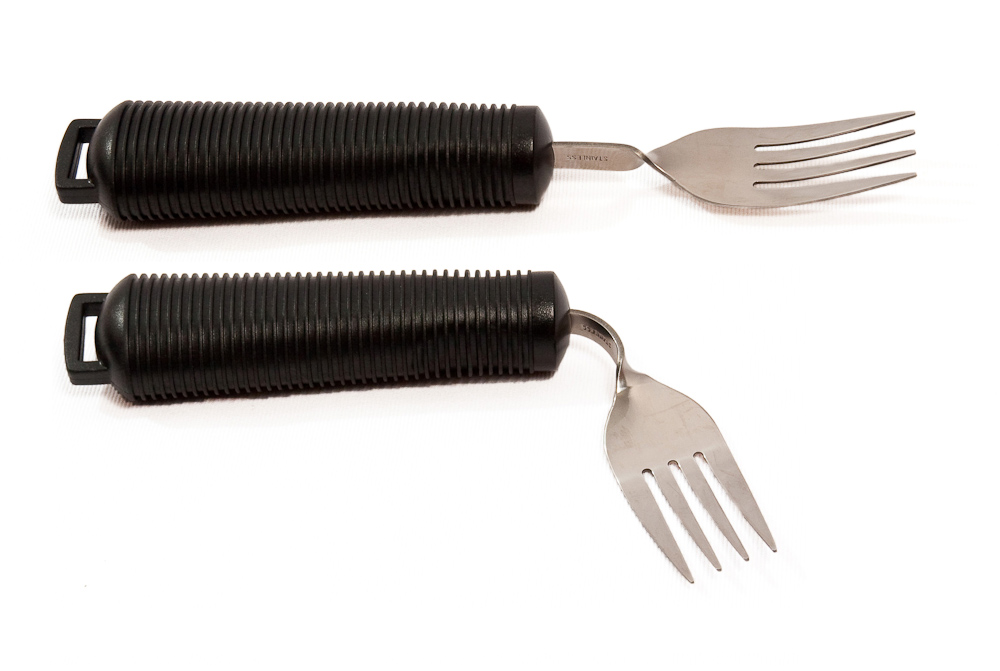
\includegraphics[width=5cm]{../figuras/talher.jpg}\\
			Fonte:\cite{vivere}
    
    \label{fig:talher}
  \end{center}
\end{figure}

A Figura \ref{fig:talher} mostra dois talheres que possuem cabos maiores para facilitar o manuseio, e um deles � ``dobrado'' para facilitar o posicionamento dos mesmos. Pacientes com quadros apresentados de Hemiplegia, Diplegia e algumas formas mistas podem se beneficiar com este tipo de talher.

}
\item{\acf{CAA}. Recursos eletr�nicos ou n�o para pessoas sem fala ou com limita��es dela (e.g., pranchas de comunica��o, vocalizadores, e softwares). A Figura \ref{fig:prancha} � um exemplo de prancha de comunica��o.

\begin{figure}[bth!]
  \begin{center}
    \caption{Exemplo de prancha de comunica��o}\vspace{.2cm}
			
      \centering
      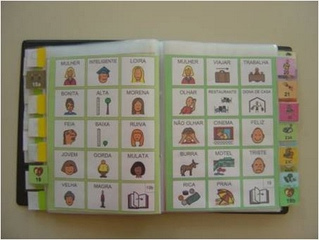
\includegraphics[width=5cm]{../figuras/prancha.jpg}\\
			Fonte:\cite{assistiva}
    
    \label{fig:prancha}
  \end{center}
\end{figure}

As pranchas de comunica��o exemplificadas na Figura \ref{fig:prancha} s�o meios de comunica��o para as pessoas com fala comprometida, isso pode ocorrer em todos os casos cl�nicos da \ac{PC}.

}
\item{Acessibilidade ao computador (e.g., teclados modificados, leitor de tela e ampliador de tela). A Figura \ref{fig:teclado} � um exemplo de teclado em modificado.
\vspace{-.5cm}
\begin{figure}[bth!]
  \begin{center}
    \caption{Exemplo de teclado em braile }\vspace{.2cm}
			
      \centering
      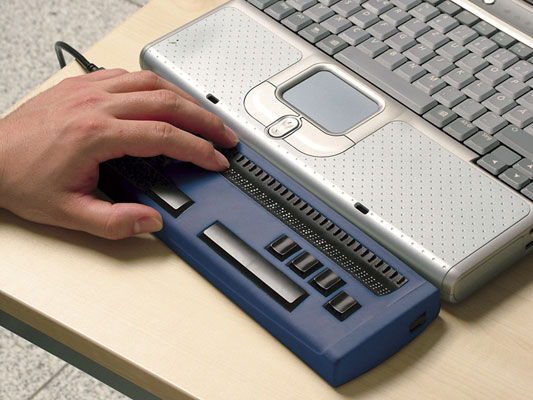
\includegraphics[width=4cm]{../figuras/teclado.jpg}\\
			Fonte:\cite{teclado}
    
    \label{fig:teclado}
  \end{center}
\end{figure}

A Figura \ref{fig:teclado} mostra que nos teclados modificados, a impress�o do que referencia cada tecla � na verdade um s�mbolo usado no alfabeto braile.

}
\item{Sistemas de controle de ambientes, que permitem que pessoas com dificuldades motoras controlem equipamentos a dist�ncia. A Figura \ref{fig:controle} � um exemplo de controle remoto para cegos.
\vspace{-.5cm}

\begin{figure}[bth!]
  \begin{center}
    \caption{Exemplo de controle assistivo}\vspace{.2cm}
			
      \centering
      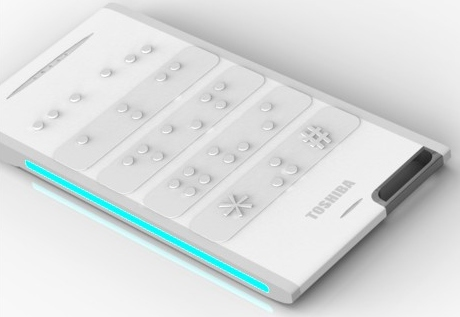
\includegraphics[width=4cm]{../figuras/controle.jpg}\\
			Fonte:\cite{controle}
    
    \label{fig:controle}
  \end{center}
\end{figure}
}
\vspace{-.5cm}
A Figura \ref{fig:controle} � um controle remoto que ao inv�s de possuir teclas com desenhos das fun��es e n�meros, os bot�es s�o representados em braile, para que os cegos possam manipular objetos a dist�ncia.

\item{Projetos Arquitet�nicos (e.g., cal�adas com guia para cegos e rampas de acesso). A Figura \ref{fig:rampa} � um exemplo de ramapa de acesso.

\begin{figure}[bth!]
  \begin{center}
    \caption{Exemplo de rampa de acesso}\vspace{.2cm}
			
      \centering
      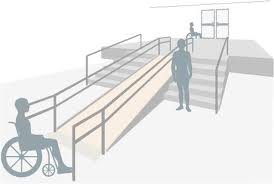
\includegraphics[width=4cm]{../figuras/rampa.jpg}\\
			Fonte:\cite{portal}
    
    \label{fig:rampa}
  \end{center}
\end{figure}

A Figura \ref{fig:rampa} representa uma rampa de acesso a cadeirantes, que torna poss�vel ao cadeirante o acesso a lugares mais elevados sem utilizar a ajuda de outras pessoas.

}
\item{�rteses e pr�teses, que permitem a troca ou ajuste de um membro. A Figura \ref{fig:protese} � um exemplo de pr�tese.
\vspace{-.5cm}
\begin{figure}[bth!]
  \begin{center}
    \caption{Exemplo de pr�tese}\vspace{.2cm}
			
      \centering
      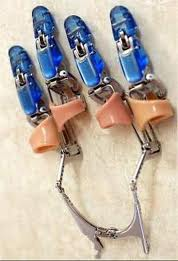
\includegraphics[width=3cm]{../figuras/protese.jpg}\\
			Fonte:\cite{protese}
    
    \label{fig:protese}
  \end{center}
\end{figure}
\vspace{-.5cm}
As pr�teses exemplificadas na Figura \ref{fig:protese}, ajudam as pessoas com membros danificados ou perdidos, a reabilita��o de movimentos.

}
\item{Equipamentos de aux�lio a postura (e.g., almofadas anat�micas e cintos). A Figura \ref{fig:cadeira} � um exemplo de cadeira de rodas com ajuste de postura.
\vspace{.5cm}
\begin{figure}[bth!]
  \begin{center}
    \caption{Exemplo de cadeira com regulagem de postura}\vspace{.2cm}
			
      \centering
      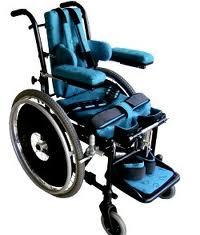
\includegraphics[width=4cm]{../figuras/cadeira.jpg}\\
			Fonte \cite{cadeira}
    
    \label{fig:cadeira}
  \end{center}
\end{figure}
}

Na Figura \ref{fig:cadeira} � poss�vel perceber o cinto na cadeira de rodas, que regulam a postura da pessoas do usu�rio.

\item{Equipamentos de mobilidade (e.g., cadeira de rodas motorizadas ou n�o e andadores). A Figura \ref{fig:cadeiramotorizada} representa um exemplo de cadeira de rodas motorizada.
\vspace{2cm}
\begin{figure}[bth!]
  \begin{center}
    \caption{Exemplo de cadeira de rodas motorizadas}
			
      \centering
      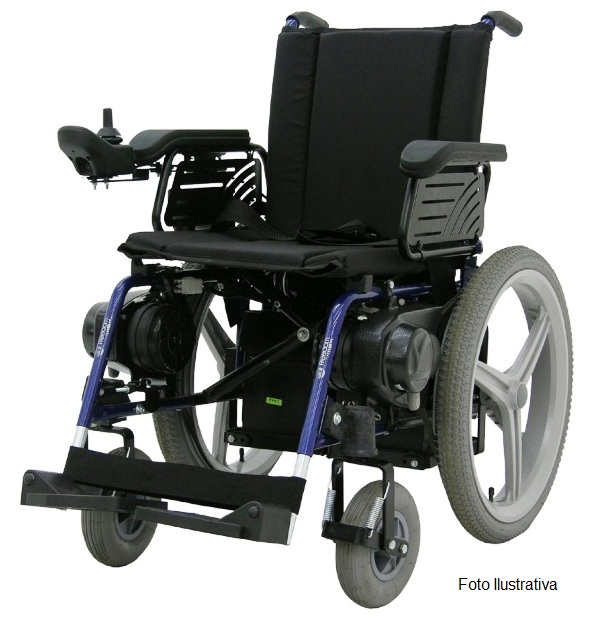
\includegraphics[width=3.5cm]{../figuras/cadeiramotorizada.jpg}\\
			Fonte: \cite{cinta}
    
    \label{fig:cadeiramotorizada}
  \end{center}
\end{figure}

Na Figura \ref{fig:cadeiramotorizada}, a cadeira possui um motor el�trico que faz com que a pessoa que a utiliza n�o necessite de grande esfor�o f�sico para moviment�-la.


}
\item{Aux�lio de surdos ou com audi��o parcial (e.g., aparelhos de surdez e telefones com teclado). A Figura \ref{fig:aparelhosurdez} � um exemplo de aparelho de surdez.
\vspace{-.5cm}
\begin{figure}[bth!]
  \begin{center}
    \caption{Exemplo de aparelho de surdez}
			
      \centering
      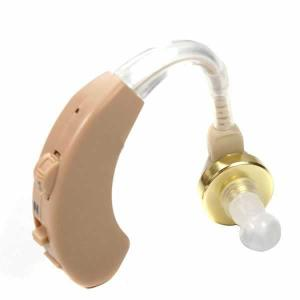
\includegraphics[width=3.5cm]{../figuras/aparelhosurdez.jpg}\\
			Fonte: \cite{surdez}
    
    \label{fig:aparelhosurdez}
  \end{center}
\end{figure}
}
\vspace{-.5cm}

Os aparelhos de surdez ilustrados pela Figura \ref{fig:aparelhosurdez} possibilitam que o �udio seja amplificado para que pessoas com defici�ncia auditiva parcial, possam escutar normalmente.

\item{Adapta��es a ve�culos. A Figura \ref{fig:carro} � um exemplo de carro adaptado a pessoas com defici�ncias f�sicas.
\begin{figure}[bth!]
  \begin{center}
    \caption{Exemplo de carro adaptado}\vspace{.2cm}
			
      \centering
      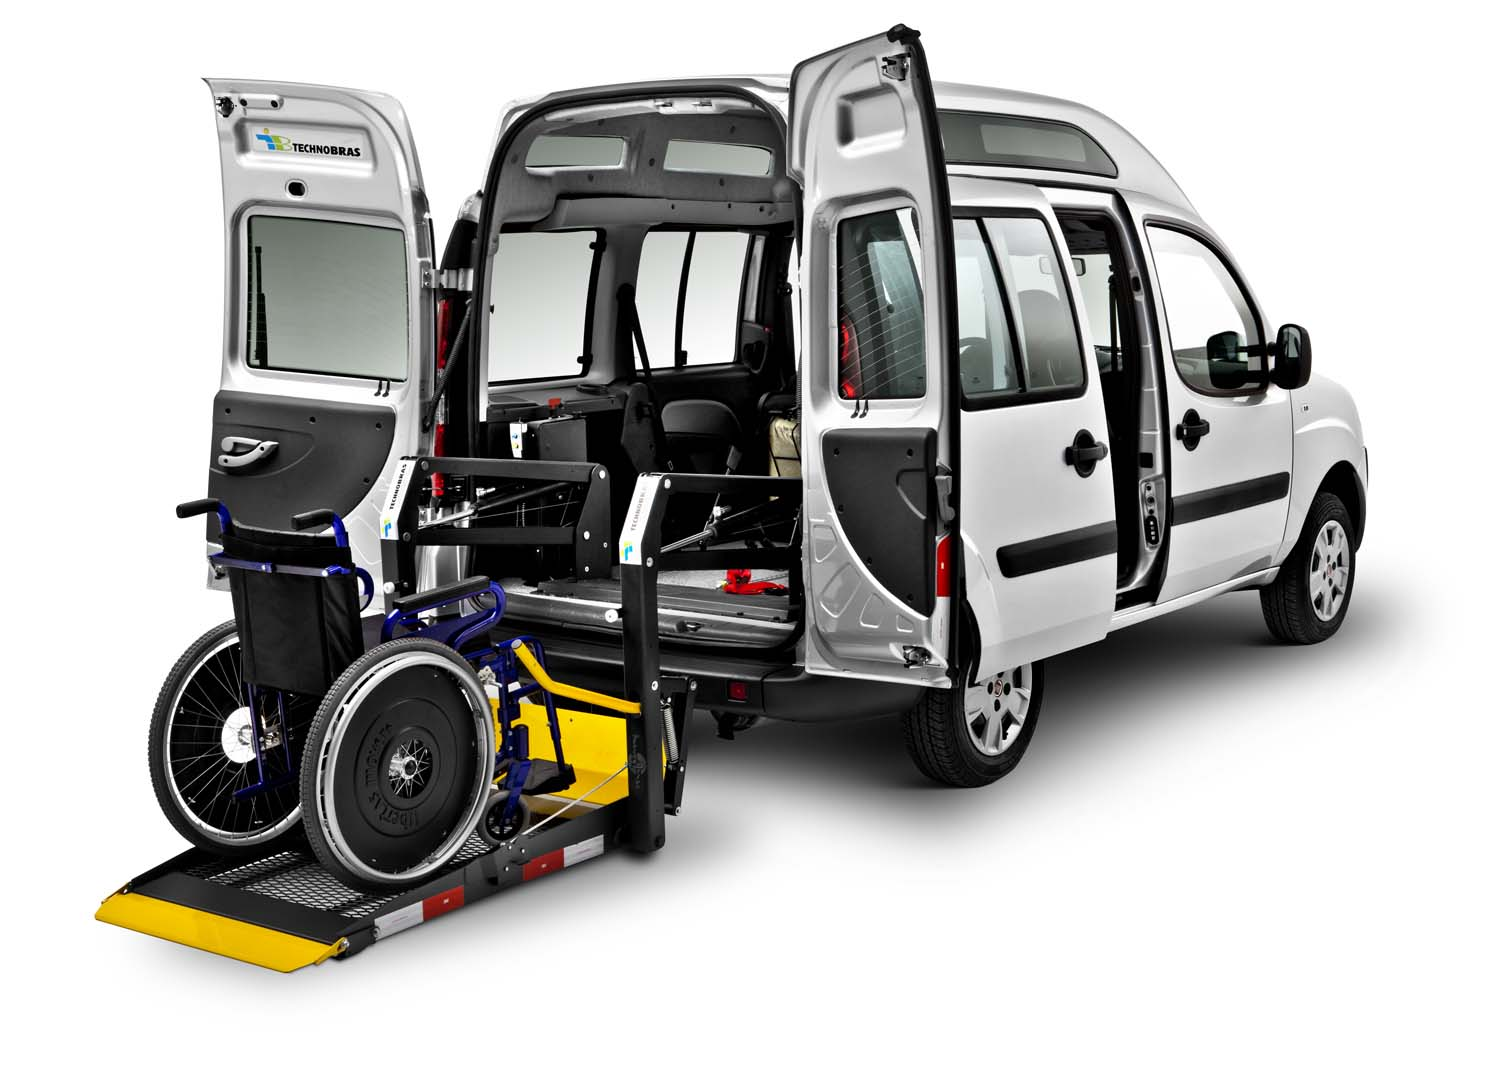
\includegraphics[width=4cm]{../figuras/carro.jpg}\\
			Fonte: \cite{fiat}
    
    \label{fig:carro}
  \end{center}
\end{figure}
}

A Figura \ref{fig:carro} � um exemplo de carro adaptado para pessoas com defici�ncia f�sica, possibilita que estas pessoas possam utilizar um ve�culo autonomamente.


\end{enumerate}


J� segundo a norma ISO 9999:2011(Anexo~\ref{iso9999}), a classifica��o das \ac{TA} se divide em categorias semelhante as diretrizes da \ac{ADA} por�m s�o mais espec�ficas. Para fins te�ricos, � utilizado no trabalho a classifica��o com base nas diretrizes da \ac{ADA} porque al�m da ISO 9999:2011 n�o incluir produtos e equipamentos usados exclusivamente por profissionais de sa�de e dispositivos implantados, a classifica��o \ac{ADA} apresenta um grupo de servi�os de \ac{TA} que promove o apoio � avalia��o da pessoa com defici�ncia, o desenvolvimento e personaliza��o de recursos, a integra��o da \ac{TA} com a��o e objetivos educacionais e de reabilita��o, e os apoios legais de concess�o \cite{corde}.


Uma pesquisa do \ac{W3C} \cite{wc} brasileiro aponta que das pessoas que usam aparelhos de \ac{TA}, 85\% � o computador o dispositivo mais usado, seguido do celular, {\it smarthphone} com 9\%, {\it tablet} com 2\%, e outros dispositivos com 4\%. Sendo cada vez mais necess�rio que existam op��es para esse tipo de p�blico dentro do acesso a informa��o.

A \ac{TA} faz parte da tecnologia, � a parte que auxilia a integra��o das pessoas que possuem algum tipo de defici�ncia. � uma �rea que envolve grandes por��es da popula��o, e que necessita de um cuidado especial, pois envolve al�m da pessoa com defici�ncia, as pessoas nos ambientes em que ela est� inserida.

\subsection{Legisla��o espec�fica de \acf{TA}}

Em rela��o a legisla��o de \ac{TA} alguns decretos s�o relevantes, entre eles a promulga��o do Decreto 3.298 
de 1999, que no artigo 19, fala do direito do cidad�o brasileiro com defici�ncia �s \ac{TA}. 
Nele consta que\cite{lima} (ver anexo {\ref{decreto1}}): 
\begin{quotation}
``Consideram-se ajudas t�cnicas, para os efeitos deste Decreto, os elementos que permitem 
compensar uma ou mais limita��es funcionais motoras, sensoriais ou mentais da pessoa 
portadora de defici�ncia, com o objetivo de permitir-lhe superar as barreiras da comunica��o e da 
mobilidade e de possibilitar sua plena inclus�o social. 
Par�grafo �nico. S�o ajudas t�cnicas:[...]elementos especiais para facilitar a comunica��o, a informa��o e a sinaliza��o para 
pessoa portadora de defici�ncia[...]``
\end{quotation}

O artigo 19 generaliza o termo Ajudas T�cnicas a todos os elementos que compensam limita��es do ser humano, por�m sem caracteriza��o ou classifica��o objetiva de tais ajudas. Tamb�m relevante, o decreto 5.296 de 2002, que d� prioridade de atendimento e estabelece normas gerais e crit�rios b�sicos para a promo��o da acessibilidade das pessoas com defici�ncia ou com 
mobilidade reduzida, possui um cap�tulo espec�fico sobre as ajudas t�cnicas no qual descreve 
v�rias inten��es governamentais na �rea da \ac{TA}, al�m de referir a constitui��o do 
\ac{CAT}. Neste decreto encontra-se que\cite{lima}: 
\begin{quotation}
``Consideram-se ajudas t�cnicas os produtos, instrumentos, equipamentos ou tecnologia 
adaptados ou especialmente projetados para melhorar a funcionalidade de pessoas portadoras de  
defici�ncia, com habilidade reduzida favorecendo autonomia pessoal, total ou assistida" .
\end{quotation}

No decreto 5.296\cite{cata} a legisla��o cita ao inv�s da compensa��o como no artigo 19, a autonomia total ou assistida das pessoas com defici�ncia. Embora esse Comit� leve a express�o ``Ajudas T�cnicas'' em sua 
denomina��o, tamb�m porque � a express�o prevista na legisla��o brasileira, 
os estudos desenvolvidos apontam e sugerem que as express�es 
``Tecnologia Assistiva'', ``Ajudas T�cnicas'' e ``Tecnologia de Apoio'', neste 
momento, continuem sendo entendidas como sin�nimos e que correspondam 
�s bases conceituais aprovadas pelo Comit�. Entretanto, estabelece a 
utiliza��o �nica da express�o ``Tecnologia Assistiva'' em seus documentos, 
como a mais apropriada, pelos seguintes motivos \apud{cata}{galvao}: 
\begin{itemize}
 
\item Por ser uma tend�ncia nacional j� firmada no meio acad�mico, nas 
organiza��es de pessoas com defici�ncia, em setores governamentais 
(Minist�rio MEC da Educa��o, Minist�rio da Ci�ncia e Tecnologia (MCT), Conselho Nacional de Desenvolvimento Cient�fico e Tecnol�gico CNPq), Institutos de Pesquisa (ITS Brasil) e no mercado de produtos; 
 
\item Pelo primeiro objetivo do Comit� de Ajudas T�cnicas, expl�cito no Artigo 
66 do Decreto 5296/2004, relativo � estrutura��o das diretrizes da �rea 
do conhecimento. A express�o Tecnologia Assistiva seria a mais 
compat�vel como a denomina��o de uma �rea de conhecimento, a ser 
oficialmente reconhecida; e
 
\item Por ser uma express�o bastante espec�fica ao conceito ao qual 
representa, diferentemente das express�es ``Ajudas T�cnicas'' e 
``Tecnologia de Apoio'', que s�o mais gen�ricas e tamb�m utilizadas para 
referirem-se a outros conceitos e realidades diferentes. 
\end{itemize}

Conforme votado e aprovado por unanimidade na quinta Reuni�o desse Comit�, al�m da determina��o de utiliza��o �nica da express�o Tecnologia Assistiva, foi decidido tamb�m que essa express�o seja utilizada no singular, por referir-se a uma �rea do conhecimento e sugere-se que se fa�am os poss�veis encaminhamentos para a revis�o da nomenclatura em 
instrumentos legais no pa�s. Este mesmo Comit� de Ajudas T�cnicas tamb�m aprovou, na sua terceira Reuni�o de abril de 2007, as bases conceituais que situam a Tecnologia Assistiva nos seguintes marcos \cite{cata,catb}: 

\begin{itemize}
\item �rea do Conhecimento;
\item Multidisciplinariedade;
\item Objetivos: promover a funcionalidade (atividade, participa��o) de 
pessoas com defici�ncia, mobilidade reduzida, ou idosas, visando sua 
autonomia, independ�ncia, qualidade de vida e inclus�o social; 
\item Composi��o: produtos, recursos, estrat�gias, pr�ticas, processos, 
m�todos e servi�os; e 
\item Ter presente os princ�pios do {\it Universal Design}\footnote{O conceito de Desenho Universal, ou ``{\it Universal Design}'', ou tamb�m chamado ``Desenho para todos'', � estudado a partir de alguns princ�pios tais como: equipara��o nas possibilidades de uso; flexibilidade no uso; uso simples e intuitivo; capta��o da informa��o; toler�ncia ao erro: m�nimo esfor�o f�sico; dimens�o e espa�o para uso e intera��o \cite{sepro}} e ITS BRASIL (Instituto de Tecnologia Social).

\end{itemize}

Apesar de uma iniciativa e uma legisla��o recente os assuntos acessibilidade e ajudas t�cnicas vem entrando no cotidiano dos brasileiros, pois h� uma cobran�a da parte governamental. Por�m, ainda existe uma defici�ncia em normas e na pr�pria legisla��o que regulamente as \ac{TA} principalmente na parte de classifica��o e exig�ncias.

\subsection{Iniciativas de \ac{TA}}
\label{iniciativas}

Existem v�rias iniciativas de \ac{TA} pelo mundo, como a  Funda��o SIDAR\cite{sidar} ({\it Seminario Iberoamericano sobre Diversidad y Accesibilidad en la Red}) que � uma institui��o de observa��o e recomenda��o na �rea da acessibilidade e inclus�o digital para os territ�rios ibero-americanos, a ATI\cite{ati} ({\it Assistive Technology Initiative}) na Universidade De George Mason na Virg�nia nos Estado Unidos, o INCNESI\cite{incnesi} (Iniciativa Nacional para os Cidad�os com Necessidades Especiais na Sociedade da Informa��o) que incentiva o uso de equipamentos para pessoas com defici�ncia em Portugal. 

Ainda no �mbito europeu, em 1999 foi organizado o Cons�rio \ac{EUSTAT} que desenvolveu um estudo entre 1997 e 1999, no contexto do Programa de Aplica��es Telem�ticas da Comiss�o Europeia, destinado a forma��o de usu�rios finais de \ac{TA}, envolvendo pessoas com defici�ncia ou idosos, seus familiares e profissionais assistentes pessoais, para que os mesmos pudessem fazer escolhas informadas, adequadas e respons�veis em rela��o a essas tecnologias. Esse estudo parte do princ�pio de que � fundamental a participa��o de usu�rio final como parceiro ativo na escolha das \ac{TA} que utiliza\cite{galvao}.

S�o parceiros do Cons�rcio \ac{EUSTAT} as seguintes organiza��es \cite{eustat}:

\begin{itemize}

\item SIVA {\it Servizio Informacione e Valutazione Ausili da Fondazione Dom Carlo Ghocchi Onlus}, da It�lia. Possui um centro de Inova��o e Transfer�ncia de Tecnologia, que incentiva projetos para autonomia de pessoas com defici�ncias;

\item CAPS  Centro de An�lise e Processamento de Sinais, do Instituto Superior T�cnico de Lisboa, Portugal;

\item \it{Association Nationale pour le Logement des personnes handicap�es}, da B�lgica;

\item \it{Groupement pour l�insertion des personnes handicap�es physiques}, da Fran�a;

\item \it{Danish Centre for Technical Aids for Rehabilitation and Education}, da Dinamarca; e

\item \it{Centro Studi Prisma}, da It�lia.

\end{itemize}

Os estudos que s�o parceiros do cons�rcio, s�o centros de refer�ncia em \ac{TA} na Europa, juntas s�o respons�veis por uma parte consider�vel de publica��es, dispositivos, sobre \ac{TA}. O Cons�rcio EUSTAT recomenda a classifica��o \ac{HEART} que prop�e tr�s grandes �reas de forma��o em 
rela��o �s \ac{TA}:
\begin{itemize} 
\item Componentes t�cnicos;
\item Componentes humanos; e
\item Componentes socioecon�micos.
\end{itemize}

Essa classifica��o tem ganhado for�a na atualidade, principalmente em decorr�ncia do paradigma inclusivo, o qual desloca as limita��es de funcionalidade e possibilidades de participa��o do �mbito restrito � defici�ncia em si, para situ�-las a partir das barreiras impostas pelo ambiente f�sico e social\cite{rodrigues}. Como n�o foi encontrado uma padroniza��o mundial para a defini��o de \ac{TA} as diferentes iniciativas encontradas se relacionam na tabela \ref{tabeladois}.

\begin{table}[bth!]
\centering
\scriptsize
\caption{Tabela com as diferen�as de Iniciativas de \ac{TA} encontradas.}\vspace{.2cm}
 \begin{tabular}{|p{2cm} |  p{3.9cm} | p{3cm} | p{4cm}| }
    \hline
    Pa�s & Termo Utilizado (Tradu��o) & Classifica��o & Defini��o \\ \hline
    Brasil & Tecnologia Assistiva, Ajudas T�cnicas &Ca\-te\-go\-ri\-as relativas aos e\-qui\-pa\-men\-tos & Melhorar as pessoas com defici�ncia e mobilidade re\-du\-zi\-da \\ \hline
    EUTSTAT & Ajudas T�cnicas e Tecnologia de Apoio & Classifica��o por componentes& Compensar as pessoas com defici�ncia e idosas \\ \hline
    ADA & {\it Assistive Technology} (Tecnologia Assistiva) & Trata as situa��es & Ajudas aos indiv�duos com defici�ncia em situa��es es\-pe\-c�\-fi\-cas \\ \hline	
		\end{tabular}
    \label{tabeladois}
		\\Fonte: o pr�prio autor.

\end{table}

A tabela {\ref{tabeladois}} mostra as diferen�as das tr�s iniciativas mais relevantes encontradas. Apesar da mudan�a de termos, as iniciativas n�o possuem grandes diferen�as entre si. A classifica��o da \ac{TA} � o �nico fator que diferencia nas iniciativas. Por�m, a relev�ncia da mudan�a � pequena, em rela��o a as ajudas �s pessoas com defici�ncia.


\section{Comunica��o Alternativa Ampliada (CAA)}

Na \ac{TA}, como mencionado anteriormente na se��o {\ref{Tecnologia Assistiva}} se divide em algumas classifica��es, dentro delas temos a \ac{CAA}, que � linha de pesquisa adotada neste trabalho. A \ac{CAA} abrange qualquer meio de comunica��o que suplemente ou substitua os m�todos naturais de fala ou escrita. � um meio que auxilia a comunica��o de um indiv�duo com outras pessoas. Os sistemas de \ac{CAA} podem ser divididos em pictoriais\footnote{Os sistemas pictoriais representam os referentes por analogia f�sica e n�o por conven��o arbitr�ria, o que lhes confere iconicidade e clareza denotativa, sendo bem compreendidos, aprendidos e lembrados por crian�as, estrangeiros e c�rebro-lesados. Contudo, o universo de significados que podem representar restringe-se ao imagin�vel \cite{fernando}.} e simb�licos\footnote{Os sistemas simb�licos representam referentes por conven��es arbitr�rias, usando regras de recombina��o e sintaxe espec�fica, o que resulta em opacidade denotativa, mas lhes permite representar virtualmente qualquer conceito, imagin�vel ou n�o \cite{fernando}.} podendo ser de alta tecnologia (e.g., sistemas computadorizados, e softwares especiais) e baixa tecnologia (e.g., simples, e n�o el�tricos) \cite{leydi}.

A \ac{CAA} � definida como uma maneira alternativa � comunica��o oral e escrita que compreende o uso de gestos, sinais manuais, express�es faciais, pranchas com s�mbolos pictogr�ficos, pranchas de alfabeto, comunicadores de voz gravada ou sintetizada at� sistemas sofisticados de computador \apud{glennen}{correia}. Inicialmente eram utilizados sistemas sem tecnologia, recorrendo apenas ao corpo humano, como a linguagem por sinais (e.g., libras) passando pelos sistemas anal�gicos ou de baixa tecnologia (e.g., cart�es e livros com s�mbolos e imagens) at� sistemas baseados em recursos computacionais (e.g., vocalizadores, e softwares para computador com s�ntese de voz) \apud{worthy}{correia}.

O trabalho da \ac{CAA} engloba uma s�rie de s�mbolos, recursos, estrat�gias e t�cnicas para auxiliar o desenvolvimento de uma comunica��o complementar. Os s�mbolos s�o as representa��es visuais, auditivas ou t�teis de um conceito; os recursos s�o os objetos ou equipamentos utilizados para transmitir as mensagens que podem ser pranchas de comunica��o, os comunicadores ou o computador; as t�cnicas s�o as formas como as mensagens s�o transmitidas e as estrat�gias referem-se ao modo como os recursos da \ac{CA} s�o utilizados \apud{king}{pelosi2}.

Como o foco deste trabalho � encontrar uma solu��o alternativa a pessoas que possuem defici�ncia na fala, em conjunto com defici�ncia motora (quadros tabela cl�nicos), a \ac{CAA} � a abordagem encontrada que melhor se encaixa neste contexto. Pois a \ac{CAA} utiliza estrat�gias e t�cnicas para o desenvolvimento de uma comunica��o complementar, que auxiliam a suplementa��o ou substitui��o da forma natural de comunica��o.


\section{Considera��es do Cap�tulo}

Com a pesquisa realizada no cap�tulo {\ref{cap:introducao}}, fica evidenciado que pessoas com necessidades especiais, precisam de recursos que supram ou compensem suas defici�ncias para que possam ser inseridas na sociedade. Apesar de uma por��o consider�vel da popula��o mundial possuir algum tipo de defici�ncia, os estudos e legisla��o sobre a \ac{TA} s�o consideravelmente recentes.
	
Al�m disso, vale ressaltar a import�ncia de que se desenvolva mais solu��es de \ac{TA}, principalmente acess�veis, e que os desenvolvedores, se preocupem com o ambiente em que esta pessoa est� inserida e as pessoas com as quais ela ir� interagir. Foram necess�rios conhecimentos sobre \ac{TA}, \ac{CAA} e acessibilidade para que se entenda o foco deste trabalho que visa encontrar uma solu��o alternativa de \ac{CAA} para pessoas que possuem \ac{PC} que apresentam defici�ncia motora e de fala.
	
Este trabalho se enquadra na Lei no 10.098, de dezembro de 2000 que estabelece crit�rios como o artigo 17 que garante direito de comunica��o e express�o por mecanismos, ou alternativas t�cnicas. Al�m disso, se enquadra tamb�m, no Decreto 5296/2004, Artigo 66 do Comit� de Ajudas T�cnicas, no qual estabelece o termo \acf{TA} como a denomina��o mais compat�vel ao tema.

O trabalho tamb�m pode ser classificado nas diretrizes da \ac{ADA} como um trabalho no contexto de \acf{CAA}. J� na norma ISO 9999:2011 na subcategoria, Produtos de Apoio para Treino de Comunica��o Alternativa e Aumentativa, c�digo 05 06 27, categoria Produtos de apoio para treino de comunica��o com imagens e desenhos.

\chapter{Cap\'itulo 2}


\chapter{Proposta para caracterização de tráfego}
\label{cap3}

Para realizar a caracterização de tráfego em uma rede é necessário coletar/medir o tráfego para posterior análise, conforme descrito na Seção~\ref{cap2:caracterizacao}.
%
Na fase de medição de tráfego é possível aplicar ferramentas existentes (\textit{e.g., } \texttt{Tcpdump}, Bro, \texttt{ping}) para recolher os dados que serão utilizados na fase de análise.
%
Contudo, por serem ferramentas amplamente difundidas e com propósito geral, estas geram dados genéricos (\textit{e.g.,} pacote inteiro), que não captam apenas os aspectos desejados para posterior análise.
%
Sendo assim, a criação de uma ferramenta de monitoramento possibilita recolher apenas os dados pertinentes a análise em questão.

Contudo, ao tratar-se da caracterização envolvendo um software complexo como o OpenStack, é necessário conhecer pelo menos a arquitetura de funcionamento dos serviços envolvidos no processo de caracterização de tráfego, conforme apresentado na Seção \ref{cap3:openstack_detalhes}.
%
Pois conhecendo o funcionamento dos serviços do OpenStack é possível entender como capturar o tráfego de interesse, quais são os seus aspectos analisáveis, e quais as melhores abordagens a adotar (Seção \ref{cap3:ambiente}).
%
Tendo estas informações em mãos, pode-se definir os requisitos para a criação do sistema de monitoramento, conforme exibido na Seção \ref{cap3:requisitos}.
%
A partir dos requisitos e das observações sobre o ambiente do OpenStack, na Seção \ref{cap3:monitoramento} é estabelecida a arquitetura do sistema de monitoramento.
%
Algumas informações geradas pelo sistema de monitoramento podem ser aplicadas diretamente para entender o tráfego, permitindo sua análise em tempo real. 
%
Contudo, certas informações necessitam de análises minuciosas, cujo processo, por exemplo, precisa que sejam feitas comparações com outras informações coletadas a fim de gerar dados significativos.
%
A fase seguinte à coleta realizada pelo sistema de monitoramento é a de análise de tráfego, cuja abordagem para o problema proposto é definida na Seção \ref{cap3:analise}.
%
Sendo explicado o que é feito com os dados coletados, e qual o tipo de informação resultante da análise.
%
Por fim, define-se na Seção \ref{cap3:experimento} como será aplicado o sistema de monitoramento, na qual explica-se os cenários de aplicação e os detalhes referentes à realização dos experimentos.

\section{Funcionamento do OpenStack}
\label{cap3:openstack_detalhes}

Conforme apresentado na Seção \ref{cap2:openstack}, a instalação do OpenStack pode distribuir os serviços entre vários hosts. 
%
Segundo a arquitetura sugerida na documentação oficial \cite{openstack:newton}, são atribuídas responsabilidades específicas para cada host da nuvem, classificados em: armazenamento, computação, controle, e de rede.
%
Estas categorias são definidas conforme os serviços executados no host, e dependendo do tamanho da nuvem, um host pode pertencer a múltiplas categorias, sendo responsável por controle e armazenamento, por exemplo.
%
No caso de nuvens maiores esta centralização é evitada por questões de desempenho.
%
A Figura \ref{fig:openstack_instalacao_servicos} apresenta uma arquitetura de instalação conceitual do OpenStack, na qual um dos hosts opera como nó de controle da nuvem e nó de rede simultaneamente.
%
Esta nomenclatura segue a utilizada na documentação do OpenStack, na qual ao referenciar-se às atribuições do host, coloca-se a palavra nó na frente, referenciando um host com serviços relacionados ao Neutron, por exemplo, como nó de rede.

\vspace{-0.3cm}
\begin{figure}[!htb]
	\centering
	\caption{Arquitetura conceitual de instalação de componentes do OpenStack}
    \vspace{-0.3cm}
	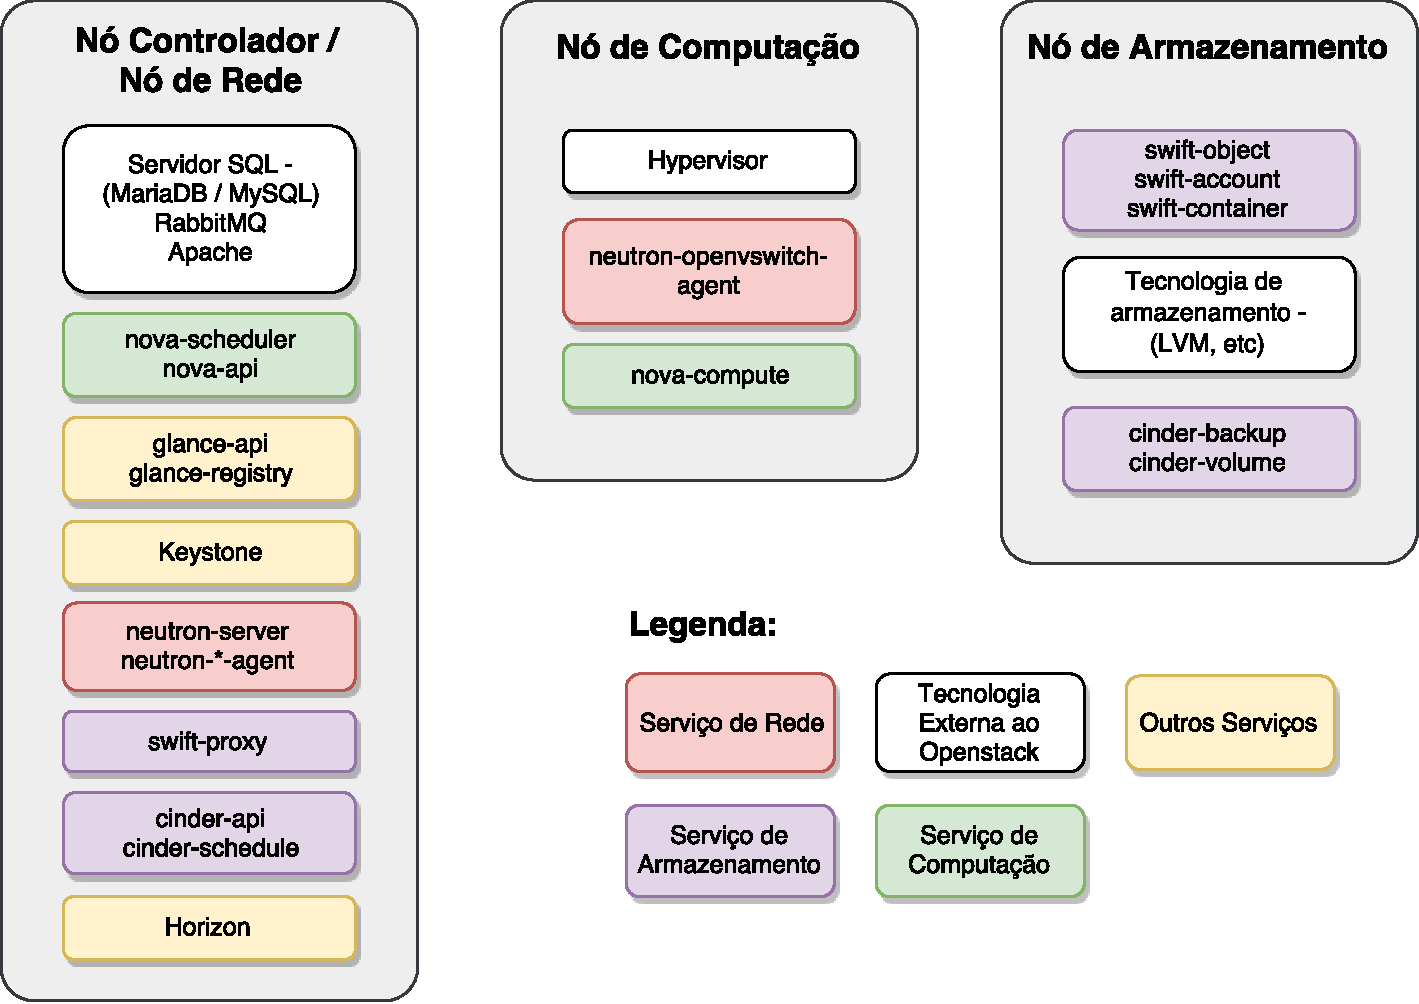
\includegraphics[width=.75\textwidth]{img/openstack_arquitetura_instalacao.pdf}
	\label{fig:openstack_instalacao_servicos}\\
    \vspace{-0.3cm}
	Fonte: O próprio autor.
\end{figure}

\vspace{-0.5cm}
Para explicitar melhor o papel de cada uma das categorias de host no tráfego de controle, esta seção apresenta brevemente como funcionam alguns serviços que executam nestes hosts, com foco na suas respectivas arquiteturas.
%
Os serviços apresentados nesta seção são os considerados no monitoramento e posterior análise do tráfego, conforme definido na Tabela~\ref{tab:openstack_service_list}, com exceção do Horizon, que é basicamente uma interface web que acessa as \acp{api} dos outros serviços, e não será abordado na explicação.
%
Esta limitação de serviços abordados visa simplificar o processo de caracterização, e segue a recomendação de serviços populares em uma instalação do OpenStack, segundo \cite{openstack:about}.



Nem todos os serviços do OpenStack têm a mesma complexidade, e neste sentido, alguns serviços como Nova e Neutron destacam-se pela complexidade.
%
Portanto, nesta seção alguns serviços mais complexos são abordados em mais detalhes do que outros com arquitetura simples (\textit{e.g.,} Keystone, Swift).
%
Além dos serviços, também é apresentada a ferramenta RabbitMQ, que possui papel importante na comunicação entre componentes pertencentes a certos serviços.
%
Esta seção inicia com o Nova, um dos serviços principais no OpenStack, que gerencia o ciclo de vida das \acp{vm} e se relaciona com vários dos serviços do OpenStack para dispor suas funcionalidades (Figura \ref{fig:openstack_service_architecture}).

\subsection{Nova}

O Nova é o serviço de computação do OpenStack, o qual gerencia os nós de computação existentes na nuvem, controlando os \textit{hypervisors} instalados nestes nós, e consequentemente, as \acp{vm} em execução. 
%
Versões anteriores do OpenStack também incluem componentes relacionados à configuração de rede no Nova (\texttt{nova-network}), que disponibiliza um modelo de gerenciamento de rede mais limitado quando comparado ao Neutron, e portanto foi descontinuado.
%
Segundo \citeonline{redhat:components}, as versão recentes do Nova utilizam uma arquitetura que divide-se em diversos componentes, conforme ilustrado na Figura \ref{fig:nova_architecture}.

\begin{figure}[!htb]
	\centering
	\caption{Arquitetura dos componentes pertencentes ao serviço Nova}
    \vspace{-0.3cm}
	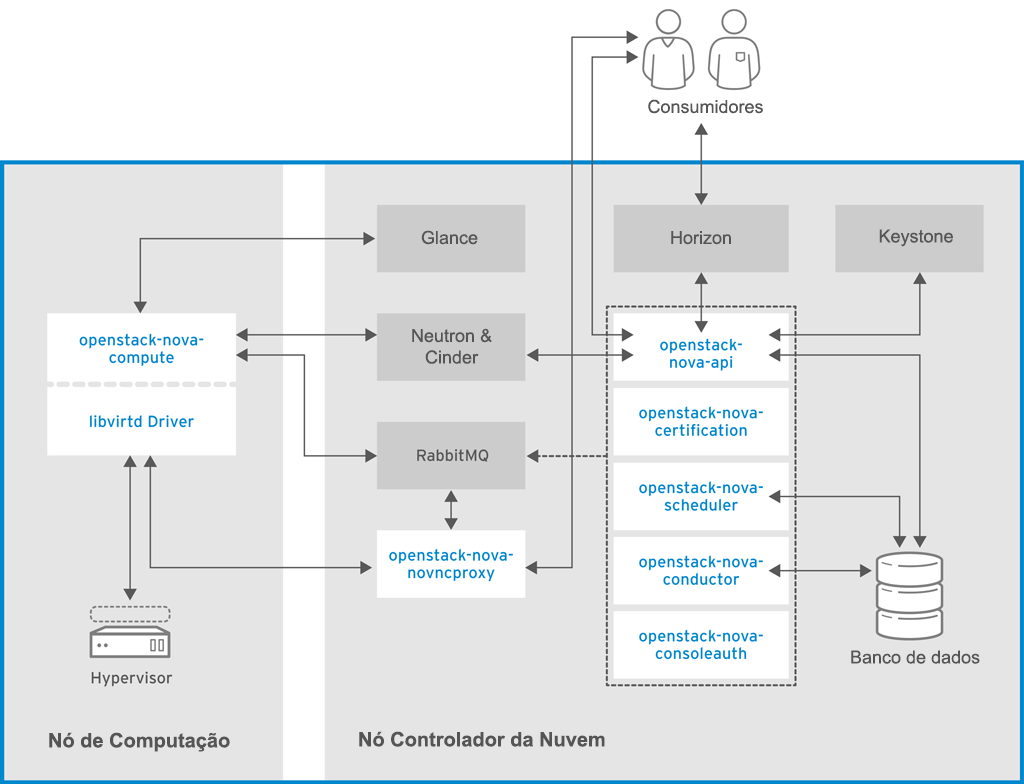
\includegraphics[width=.8\textwidth]{img/nova_arquitetura.png}
	\label{fig:nova_architecture}\\
	Fonte: Adaptado de \cite{redhat:components}.
\end{figure}

Apesar dos vários componentes pertencentes ao serviço Nova (Figura \ref{fig:nova_architecture}), este trabalho foca em alguns componentes principais: \ac{api}, escalonamento, computação, banco de dados, e \textit{message broker} (AMQP Server).

Conforme apresentado na Seção \ref{cap2:openstack}, a \ac{api} do Nova (\texttt{nova-api}) é responsável por disponibilizar acesso e tratar requisições para o serviço Nova.
%
O \texttt{nova-api} em sua essência é um \textit{Web Service} implementado sobre o protocolo REST, e gerencia autorização e funções básicas de controle, na qual implementa modelos de API compatíveis como o da Amazon e Rackspace.
%
Existem diferentes versões da REST \ac{api} do Nova, que introduzem novas funcionalidades ou padronizações, o OpenStack Newton por exemplo, que é a versão que este TCC irá trabalhar, tem a REST \ac{api} do Nova na versão 2.38 \cite{openstack:newton:api}.
%
Toda requisição recebida pelo \texttt{nova-api} é avaliada para verificar se os recursos referenciados na requisição estão disponíveis, e caso estiverem disponíveis, a requisição é enviada ao \textit{message broker}, que é um servidor \acf{amqp}, e disponibiliza a mensagem para os recursos referenciados acessarem \cite{openstack:nova}.
%
O \textit{message broker} é um \textit{middleware} com o protocolo \ac{amqp} utilizado para comunicação interna entre componentes de certos serviços, que no caso do Nova por exemplo, se aplica aos componentes \texttt{nova-scheduler} e \texttt{nova-compute}, e também intermedeia o acesso ao banco de dados pelo \texttt{nova-compute}.

Durante a troca de mensagens, o \textit{message broker} também atualiza o banco de dados do Nova, que mantém informações sobre o estado corrente da nuvem, como por exemplo, o números de \acp{vm} executando em cada nó de computação da nuvem \cite{redhat:components}.
%
Este banco de dados é implementado em MySQL e é acessível pelos componentes do Nova, o qual centraliza as informações que os componentes necessitam durante sua execução.
%
Após receber a mensagem contendo o pedido de \ac{vm} pelo \textit{message broker}, o componente responsável pelo escalonamento, chamado \texttt{nova-scheduler} define qual nó de computação hospedará uma nova instância de \ac{vm}.
%
Para definir o nó de computação é consultado o banco de dados do Nova, que contém informações aplicáveis no processo de filtragem para encontrar um nó de computação disponível para hospedar a \ac{vm}.
%
Neste sentido, é possível fornecer pesos para as métricas, ajudando na escolha do nó de computação, como também é possível deixar a escolha aleatória entre os nós de computação filtrados no processo, que correspondem aos nós de computação podendo hospedar aquela \ac{vm} \cite{openstack:nova}.

No caso de uma nuvem de pequeno porte, os componentes do Nova exibidos até aqui executam em um mesmo nó de controle, pois não necessitam de grande quantidade de processamento.
%
Em contraste, o componente \texttt{nova-compute} executa em cada host que contém um \textit{hypervisor}, ou seja, um nó de computação, e é responsável por gerenciá-los.
%
Como todos os outros componentes do Nova que usam \ac{amqp}, o \texttt{nova-compute} em execução verifica periodicamente por tarefas enfileiradas para ele, e realiza-as conforme solicitado (\textit{e.g.,} criar instância, finalizar instância, ler saída do \textit{console}).
%
Se outros serviços que dispõem funcionalidades extras às \acp{vm} estiverem instalados (\textit{e.g.,} Cinder, Glance, Neutron), cada \texttt{nova-compute} realiza a comunicação direta com estes serviços.


\subsection{Cinder}

Para disponibilizar armazenamento persistente às \acp{vm}, o serviço Cinder permite acoplar volumes/blocos de armazenamento nas \acp{vm} em execução.
%
Além de disponibilizar armazenamento para \acp{vm}, o Cinder também fornece a habilidade de criar \textit{snapshots} dos volumes de armazenamento, que copia o conteúdo do volume, e possibilita gerar novos volumes contendo os dados deste \textit{snapshot}.
%
Mesmo sendo mais simples que o Nova, o Cinder também emprega múltiplos componentes para realizar suas funções, que podem ser distribuídos entre diferentes hosts.
%
Alguns componentes com comportamento similar aos componentes do Nova estão presentes: escalonador, banco de dados, \ac{api} e \textit{message broker}; em que difere-se nos componentes responsáveis pelo armazenamento: \texttt{cinder-backup} e \texttt{cinder-volume}.

O papel do \texttt{cinder-api}, componente que gerencia a \ac{api} do Cinder, é disponibilizar uma interface REST para que os outros serviços do OpenStack, como o Nova, acessem suas funcionalidades \cite{redhat:components}.
%
A REST \ac{api} do Cinder encontra-se na v3.15 no OpenStack Newton \cite{openstack:newton:api}.
%
Após recebido o pedido pelo \texttt{cinder-api}, ele é enviado ao \textit{middleware} responsável pela comunicação entre os componentes, baseado no protocolo \ac{amqp}, e que não necessita ser de uso exclusivo do Cinder.

O banco de dados, baseado em MySQL, tem propósito similar ao banco de dados no Nova: compartilhar informações relacionadas ao estado atual do serviço para os componentes, na qual também pode usar o mesmo servidor de banco de dados.
%
O escalonador \texttt{cinder-scheduler} decide onde armazenar volumes e backups criados, cuja funcionalidade é disponibilizada pelos componentes \texttt{cinder-volume} e \texttt{cinder-backup}, que podem ser hospedados em múltiplos hosts, servindo como nós de armazenamento.
%
Segundo \citeonline{redhat:components}, estes dois componentes podem usar várias soluções de armazenamento (\textit{e.g.,} Ceph, LVM, NFS), e em especial o \texttt{cinder-backup} é capaz de armazenar seus backups no Serviço de armazenamento Swift.

\subsection{Swift}

O Swift é outro serviço do OpenStack responsável pelo armazenamento, mas com o foco em armazenar dados estáticos de grande volume (\textit{e.g.,} vídeos, imagens, imagens de \ac{vm}).
%
O acesso aos dados é feito com o um pedido HTTP (\texttt{Get, Put, Delete}) para o \texttt{swift-proxy}, que é o componente do Swift responsável pela \ac{api}, e autenticação no serviço, que no OpenStack Newton encontra-se na v1 \cite{openstack:newton:api}.
%
Ao receber uma requisição é consultado a localização do objeto nos outros componentes (\texttt{swift-account}, e \texttt{swift-container}, respectivamente), roteando então a requisição de acordo com as informações consultadas, conforme ilustrado na Figura \ref{fig:swift_components}.

O Swift tem dois componentes que gerenciam acesso a listagem de informações: o \texttt{swift-account}, que gerencia a lista de contêineres de armazenamento no banco de dados, e o \texttt{swift-container}, cuja tarefa é gerenciar a lista de objetos contidos nos contêineres, também armazenado no banco de dados.
%
Para gerenciar os objetos armazenados, o componente \texttt{swift-object} armazena, recupera e exclui objetos conforme requisitado \cite{openstack:swift}.
%
A parte de autenticação do \texttt{swift-proxy} comunica-se com o serviço Keystone, que fornece uma \ac{api} que centraliza o processo de autenticação do OpenStack.

\begin{figure}[!htb]
	\centering
	\caption{Arquitetura dos componentes pertencentes ao serviço Swift}
    \vspace{-0.3cm}
	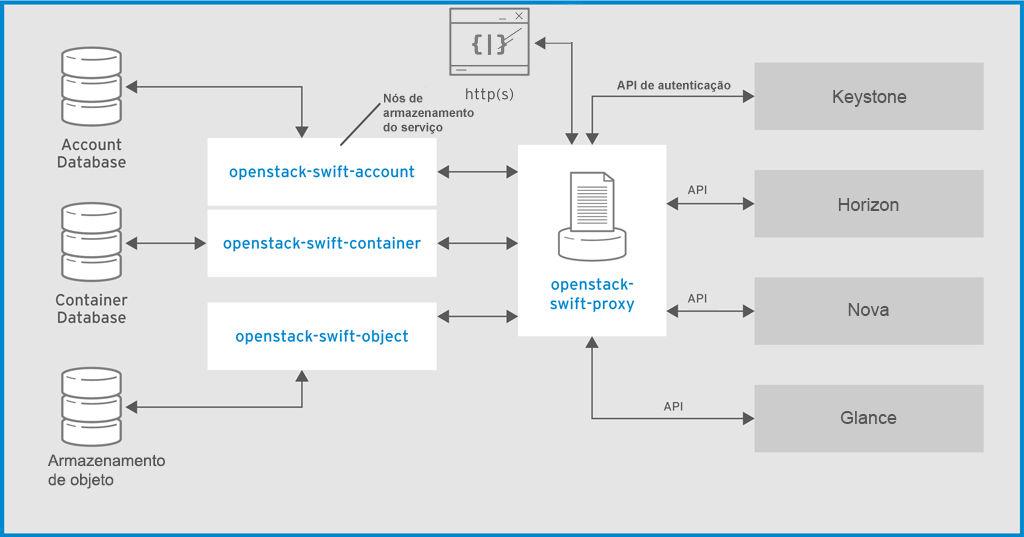
\includegraphics[width=.8\textwidth]{img/swift_arquitetura.png}
	\label{fig:swift_components}\\
	Fonte: Adaptado de \cite{redhat:components}.
\end{figure}

\subsection{Keystone}

O serviço Keystone fornece autenticação e autorização aos serviços do Openstack. 
%
Este serviço possibilita a autenticação através de múltiplos mecanismos, como por exemplo, credencial com usuário e senha, ou através de \textit{tokens} \cite{redhat:components}.
%
Desta maneira, é possível combinar estes mecanismos no uso do Keystone, no qual um pedido de autenticação é validado através de usuário e senha, e então, o serviço pode retornar um \textit{token} ao solicitante, que é utilizado para a autenticação posteriormente \cite{openstack:keystone}.

A arquitetura de funcionamento do Keystone é relativamente simples, possuindo apenas um componente principal, que é responsável pela \ac{api} do serviço, e encontra-se na v3 no OpenStack Newton.
%
A \ac{api} do Keystone armazena as identidades, autorizações, catálogos de serviços e \textit{tokens} no MySQL (MariaDB) por padrão, podendo-se adicionar outras tecnologias para cuidar de partes específicas do serviços. 
%
Neste sentido, a tecnologia \ac{ldap} pode ser empregada no gerenciamento de autenticações e \textit{memcache} ou \textit{Redis} para gerenciar a persistência dos \textit{tokens} \cite{redhat:components}.
%
Após autenticado o usuário (consumidor ou administrador), ele é capaz de acessar o catálogo fornecido pelo Keystone, cuja funcionalidade é armazenar os serviços em funcionamento no Openstack, e informar ao usuário quais recursos ele pode acessar.


\subsection{Glance}

O serviço Glance funciona como um registro de imagens de \acp{vm} acessível pelos consumidores da nuvem. 
%
É possível que os consumidores adicionem novas imagens, desde que estas sejam em um dos formatos aceitos pelo serviço, que segundo \citeonline{redhat:components}, inclui \texttt{iso}, \acp{vm} do VirtualBox (\texttt{vdi}), VMware (\texttt{vmdk}) e Amazon EC2 (\texttt{ami}).
%
Outra alternativa é gerar um \textit{snapshot} a partir de uma das \acp{vm} do consumidor, que pode servir como \textit{backup} ou imagem para iniciar outras \acp{vm}.

Em relação à sua arquitetura, o Glance é dividido nos seguintes componentes principais \cite{openstack:glance}: \texttt{glance-api}, \texttt{glance-registry}, repositório de armazenamento e banco de dados (MySQL/MariaDB).
%
A \ac{api} do Glance (\texttt{glance-api}) gerencia todos os pedidos para recuperação e armazenamento de imagens, que no OpenStack Newton tem a \ac{api} v2 \cite{openstack:newton:api}.
%
Enquanto os pedidos são processados, o componente \texttt{glance-registry} acessa o banco de dados instalado para buscar informações da imagem em questão (\textit{e.g.,} metadados da imagem, local de armazenamento).
%
As imagens registradas neste serviço podem ser armazenadas no serviço Swift ou através de outras tecnologias como RADOS Block Service, VMware datastore, HTTP, ou até como arquivo no próprio sistema de arquivos do host do Glance.


\subsection{Neutron}

Conforme apresentado na Seção \ref{cap2:openstack_network_architecture}, uma das funcionalidades do serviço Neutron é fornecer rede às \acp{vm} dos consumidores, incluindo a possibilidade de configurar a rede em questão, sub-redes e os seus roteadores \cite{redhat:components}.
%
Outras funcionalidades adicionais também podem ser oferecidas para a rede criada em um \textit{project}/\textit{tenant}, como DHCP (\texttt{neutron-dhcp-agent}), \textit{Firewall} ou \acp{vpn}.

\begin{sloppypar}
Comparado com os outros serviços do OpenStack, o Neutron é um dos mais complexos, podendo envolver diversas tecnologias de rede e possibilidades de configuração \cite{denton:2016:neutron}.
%
No geral, o Neutron tem os seguintes componentes: \textit{Network agents}, que inclui os componentes \texttt{neutron-dhcp-agent}, \texttt{neutron-openvswitch-agent} e \texttt{neutron-l3-agent}; \texttt{neutron-server} e \textit{message broker} \cite{openstack:neutron}.
%
Os \textit{Network agents} executam em todos os hosts de uma nuvem OpenStack, e são responsável por cuidar, por exemplo, da configuração das \acp{vm} contidas no host e também de serviços e \textit{plugins} em execução no Neutron, como o Open vSwitch (\texttt{neutron-openvswitch-agent}).
%
O Open vSwitch é uma das tecnologias que pode ser empregada na virtualização das interfaces de rede físicas dos hosts, e permite criar \acp{vlan} para isolar o tráfego de cada rede.
%
Assim, é possível que o tráfego de dois domínios diferentes trafeguem no mesmo meio físico com isolamento.
\end{sloppypar}

O componente \texttt{neutron-ml2} (Modular Layer 2) é obrigatório no Neutron, e controla a Camada 2 da rede, ou seja, encaminha pacote apenas dentro das redes criadas pelos consumidores.
%
A nível estrutural, o \texttt{neutron-ml2} funciona como um \textit{framework} que possibilita a criação de \textit{plugins} que relacionam-se com a Camada 2 da rede, como o TaaS (\textit{Tap-as-a-Service})\footnote{\url{https://github.com/openstack/tap-as-a-service}}, por exemplo.
%
O TaaS possibilita a criação de espelhamentos de portas das redes dos consumidores da nuvem, que tornam-se acessíveis através de portas virtuais criadas pelo TaaS no Open vSwitch, cuja aplicação inclui, por exemplo, o monitoramento do tráfego com um \ac{ids}.
%
Para fornecer acesso à rede externa um \textit{L3 Network agent} (\texttt{neutron-l3-agent}) deve executar no nó de rede da nuvem, e responsabilizar-se pelo roteamento dos pacotes para fora da rede do consumidor, que corresponde à função do roteador virtual inserido pelo consumidor na sua rede \cite{redhat:components}.
%
O agente DHCP (\texttt{neutron-dhcp-agent}) é outro agente que executa no nó de rede, e fornece o serviço de DHCP para as redes dos consumidores.

Por fim, o componente \texttt{neutron-server} é responsável pela \ac{api} do serviço, que age similar aos outros serviços, na qual envia as mensagens para o \textit{message broker}, que encaminha-as para os outros agentes e \textit{plugins} do Neutron.
%
Através da sua \ac{api} os consumidores definem as configurações das suas redes, e o administradores definem as tecnologias de redes empregadas nos serviços do Neutron \cite{denton:2016:neutron}.
%
A \ac{api} do Neutron encontra-se na v2 atualmente, e é a mesma utilizada no OpenStack Newton, na qual baseia-se em um aprimoramento da \ac{api} do Quantum (serviço de rede descontinuado) na v1.1 \cite{openstack:newton:api}.


\subsection{RabbitMQ}

Conforme apresentando nos serviços Neutron, Cinder e Nova, é necessário haver um servidor responsável pela comunicação interna destes serviços, ou seja, entre os seus componentes.
%
O OpenStack emprega o protocolo \ac{amqp} para realizar esta comunicação interna, cujas mensagens são criadas no padrão do protocolo \acf{rpc}, que é implementado pelo projeto Oslo.
%
Neste sentido, o servidor \ac{amqp} (\textit{e.g.,} RabbitMQ, Qpid, ZeroMQ), também chamado de \textit{message broker} apenas transporta a mensagem, seguindo o padrão \textit{publish/subscribe}.
%
A utilização deste \textit{middleware} para comunicação tem como objetivo \cite{openstack:amqp_cinder}: desacoplar o host de origem e destino da mensagem; completo assincronismo entre os hosts (não é necessário que o destino esteja disponível ao enviar mensagem); balanceamento entre chamadas remotas (mensagem é recebida pelo primeiro host disponível a acessar o RabbitMQ). 

Neste meio de comunicação exitem dois tipos de chamadas: \textit{RPC Call} e \textit{RPC Cast} \cite{openstack:amqp_cinder, openstack:amqp_nova}.
%
No \textit{RPC Call}, é enviada uma mensagem do host, e então cria-se um \textit{Consumer} neste host, que escutará a resposta da execução remota, sem efetuar bloqueio no processo de espera.
%
Para saber a quem cada resposta pertence, um campo \texttt{msg\_id} é criado ao enviar a primeira mensagem, e assim o \textit{Publisher} sabe que aquela resposta é para ele.
%
No \textit{RPC Cast}, o método é invocado remotamente, mas sem escutar a resposta de quem o executou.
%
O envio pelo \textit{Publisher} e recebimento de mensagens pelo \textit{Consumer} é separado por tópico, e só os hosts com certo componente ou serviço em execução recebe mensagens de certo tópico.
%
A arquitetura do OpenStack não diferencia os hosts conectados ao RabbitMQ, contudo, é possível verificar uma diferença em comportamento neles, na qual alguns hosts enviam mais mensagens, enquanto outros ficam responsáveis por receber e processar as mensagens.
%
Este tipo de comportamento pode ser verificado ao comparar hosts que executam o \texttt{nova-api} e o \texttt{nova-compute}, por exemplo, em que a \ac{api} repassa tarefas a serem realizadas para outros componentes do Nova, como o \texttt{nova-compute}, que fica à escutar por novas tarefas que deva executar.

\subsection{Considerações OpenStack}
Conhecidos alguns serviços do OpenStack, o próximo passo para a criação do sistema de monitoramento é analisar aspectos específicos de nuvens OpenStack de maneira que auxilie a definir o funcionamento do sistema de monitoramento proposto.
%
Ou seja, objetivo da análise do ambiente de caracterização é definir algumas diretrizes úteis posteriormente: qual é o tráfego de interesse, quais são algumas das características observáveis neste tráfego de interesse, e quais são os locais da rede com maior concentração deste tráfego.

\section{Ambiente de caracterização}
\label{cap3:ambiente}

A Seção \ref{cap3:openstack_detalhes} apresenta a arquitetura de alguns serviços do OpenStack incluídos na caracterizar de tráfego deste TCC.
%
Sendo assim, a partir de suas características de funcionamento podem ser definidas estratégias para criar o sistema de monitoramento responsável por medir o tráfego e o analisar (Seção \ref{cap2:caracterizacao}).
%
O propósito desta seção é exibir características do OpenStack apresentadas neste TCC que podem ser exploradas na construção do sistema de monitoramento.

As \acp{api} dos serviços do OpenStack são responsáveis por expor suas funcionalidades aos consumidores da nuvem e a outros serviços.
%
Neste sentido, toda ação realizada na nuvem por algum consumidor inicia-se através da comunicação com a \ac{api}.
%
Após a realização de um pedido através da \ac{api}, o serviço correspondente retorna uma mensagem informando sobre o \textit{status} da ação realizada (\textit{e.g.,} sucesso, falha, informações à respeito).
%
Logo, é possível descobrir se o consumidor foi capaz de realizar certa ação ao olhar a resposta recebida.
%
Sendo assim, monitorar as mensagens que passam pelas \acp{api} em busca de comportamentos de interesse é uma maneira de entender o que ocorre na nuvem.
%
A Figura \ref{code:nova_api_response} apresenta uma resposta ao realizar uma consulta para a \ac{api} do Nova (\texttt{nova-compute}) solicitando a lista de volumes fornecidos pelo Cinder que estão acoplados em uma certa \ac{vm}.

\begin{figure}[!htb]
	\centering
    \caption{Exemplo de resposta recebida ao consultar volumes de armazenamento acoplados a uma instância do Nova}
    \begin{minted}{json}
{
    "volumeAttachments": [
        {
            "device": "/dev/sdd",
            "id": "a26887c6-c47b-4654-abb5-dfadf7d3f803",
            "serverId": "4d8c3732-a248-40ed-bebc-539a6ffd25c0",
            "volumeId": "a26887c6-c47b-4654-abb5-dfadf7d3f803"
        },
        {
            "device": "/dev/sdc",
            "id": "a26887c6-c47b-4654-abb5-dfadf7d3f804",
            "serverId": "4d8c3732-a248-40ed-bebc-539a6ffd25c0",
            "volumeId": "a26887c6-c47b-4654-abb5-dfadf7d3f804"
        }
    ]
}
	\end{minted}
    \label{code:nova_api_response}
    Fonte: \cite{openstack:nova_api_response}.
\end{figure}

A resposta segue o padrão REST, e é formatado com JSON, na qual pode-se aplicar ferramentas de \textit{parse} ou análise com expressão regular para extrair informações.
%
No caso de falha, por exemplo, esta mensagem no protocolo HTTP poderia retornar algum código de erro, como o código 401 (\texttt{unathorized}) caso o solicitante não tenha permissão para acessar a informação \cite{openstack:nova_api_response}.

A partir do monitoramento da \ac{api} é possível visualizar a requisição de uma ação na nuvem e a resposta resultante do sistema.
%
Ou seja, enxerga-se a nuvem como uma caixa preta, observando a entrada e a saída resultante da \ac{api}.
%
Para aumentar a quantidade de informações disponíveis, é possível observar o conteúdo desta ``caixa preta'' através do monitoramento da comunicação entre componentes de um serviço.

Serviços complexos como o Nova, Neutron e Cinder possuem componentes distribuídos pela nuvem, e a responsabilidade da comunicação entre estes componentes fica a cargo do \textit{middleware} de comunicação (RabbitMQ).
%
Conforme apresentado na Seção \ref{cap3:openstack_detalhes}, quando um componente de algum serviço como o Nova enviar uma mensagem \ac{rpc} para o RabbitMQ, a mensagem é recebida por um componente com interesse nela (tópico da mensagem).
%
Contudo, uma mensagem enviada para o RabbitMQ pode esperar certo tempo até ser recebida por algum destino, pois algum dos destinos em potencial deve verificar se há alguma mensagem de interesse disponível para receber do \textit{middleware} de comunicação.
%
Sendo assim, ao monitorar as mensagens \textbf{saindo} do RabbitMQ pode-se ter certeza que aquelas mensagens serão processadas logo em seguida pelo destino.

O sistema de monitoramento de \cite{sharma:2015:hansel} analisa o tráfego \ac{rpc} e REST, com o objetivo de organizá-lo numa sequência de mensagens que representa um evento na nuvem.
%
A sequência é criada ao encontrar várias mensagens com o mesmo identificador, que segundo \cite{sharma:2015:hansel}, o OpenStack utiliza para controle interno.
%
Portanto, é possível relacionar requisições dos consumidores da nuvem e as subsequentes comunicações entre os componentes para executá-las.
%
Porém, uma dificuldade encontrada por \cite{sharma:2015:hansel} ao analisar mensagens \ac{rpc} é a ausência de uma maneira simples de indicar a presença de erro.
%
Uma estratégia de uso para empregar ambos os protocolos pode consistir da análise de mensagens REST em direção à \ac{api}, e então de acordo com o tipo de ação, caso houver necessidade de acompanhar o processo detalhadamente, pode-se analisar o tráfego RPC gerado em função desta requisição REST.

Serviços do OpenStack executam por padrão na rede de controle com as portas definidas segundo a Tabela \ref{tab:openstack_service_list}, e não mudam durante a execução.
%
Logo, é possível associar cada pacote de controle na nuvem ao serviço do OpenStack de destino através da porta de destino definida no cabeçalho do pacote.
%
Mesmo este método de classificação sendo simples, com ele é possível realizar uma medição que classifica, por exemplo, os serviços do OpenStack que recebem mais mensagens.
%
Contudo, para garantir que a classificação apresente resultados significativos é necessário isolar o tráfego de armazenamento.
%
A justificativa é que a transferência de uma imagem de \acp{vm} ou de um volume de armazenamento, por exemplo, é feita com vários pacotes, podendo impactar significativamente a medição realizada.

Em relação ao processo de coleta de tráfego, ou seja, na fase de medição do tráfego da rede de controle, é necessário que a abordagem meça o tráfego gerado pelo OpenStack.
%
Com isso em mente, a medição ativa possui pouca aplicabilidade, pois o princípio desta abordagem é justamente depender apenas do tráfego gerado pelo próprio software de monitoramento, descartando a necessidade de conhecer características da rede (\textit{e.g.,} topologia, comportamento) cuja medição será realizada.
%
Portanto, no caso da rede de controle de uma nuvem OpenStack, por exemplo, a medição de tráfego passiva é a melhor escolha, visto que diferente da abordagem ativa, a medição passiva coleta todo o tráfego no ponto de medição, que na rede de controle é gerado apenas pelo OpenStack e tecnologias relacionadas.

Escolhida a abordagem de medição passiva, o próximo passo é decidir sobre o ponto de medição, que pode ser distribuído em vários pontos da rede dependendo da necessidade.
%
Considerando o que foi apresentado sobre o tráfego \ac{rpc} e REST no começo desta seção, por exemplo, deve-se escolher um ou mais pontos de coleta de maneira que a medição cubra o máximo de tráfego de interesse quanto possível (\textit{e.g.,} mensagens em \ac{rpc} e REST).
%
Neste sentido, conforme ilustrado na Figura \ref{fig:openstack_instalacao_servicos}, os serviços do OpenStack e outras tecnologias relacionadas com as \acp{api} e comunicação interna de serviços (\textit{e.g.,} RabbitMQ) são distribuídas entre nós de rede e de controle da nuvem.
%
Logo, os nós de rede e de controle de uma nuvem OpenStack são potencialmente bons locais para posicionar a parte responsável pela medição de tráfego no sistema de monitoramento.
%
%Definidas algumas das abordagens possíveis para monitorar o tráfego com base nas características observadas, a Seção \ref{cap3:monitoramento} aplica algumas destas informações na criação do sistema de monitoramento.


\section{Especificação de requisitos}
\label{cap3:requisitos}

Com o objetivo de solucionar o problema de caracterização de tráfego, abordado na Seção \ref{cap2:problema}, esta seção inicia a proposta de solução apresentando alguns requisitos que devem ser considerados na proposta.
%
Estes requisitos estão associados à primeira parte do processo de caracterização de tráfego proposto, que é a medição de tráfego, e que será de responsabilidade do sistema de monitoramento.
%
Sendo assim, existem pré-requisitos para possibilitar que o sistema de monitoramento realize a medição de tráfego corretamente:

\begin{itemize}
	\item Ter acesso ao tráfego que passa pelas interfaces de rede, físicas e virtuais, da nuvem monitorada;
    %\item O dispositivo monitorado deve ter memória suficiente disponível;
    \item Um dispositivo de monitoramento necessita estar conectado à rede de controle da nuvem que pertence; e
    \item Existir um banco de dados de dados acessível para armazenar os dados gerados.
\end{itemize}

Os requisitos são abstrações de funcionalidades que monitoram aspectos observáveis na rede de controle.
%
Estes aspectos monitorados serão consultados na fase de análise do tráfego.
%
Os requisitos que devem possibilitar a medição do tráfego da rede de controle, a fim de gerar informações sobre aspectos observáveis do tráfego são divididos em requisitos funcionais e requisitos não funcionais:

Requisitos funcionais:
\begin{itemize}
	\item \textbf{RF1.} Contabilizar o consumo de tráfego na rede de controle dos serviços em execução;
    \item \textbf{RF2.} Armazenar a comunicação entre os componentes dos serviços em execução;
    \item \textbf{RF3.} Armazenar as requisições recebidas pelas \acp{api}, originárias tanto de consumidores quanto de outros serviços; e
    \item \textbf{RF4.} Os dados devem ser detalhados, de maneira que eles revelem tarefas responsáveis por variações na nuvem.
\end{itemize}

Requisitos não funcionais:
\begin{itemize}
	\item \textbf{RNF1.} Operar independente do OpenStack, não sendo atrelado a uma implementação de nuvem apenas; e
    %\item Ser fácil de implementar;
    \item \textbf{RNF2.} O sistema de monitoramento não pode impactar no desempenho da nuvem sendo analisada.
\end{itemize}


\section{Proposta de sistema de monitoramento}
\label{cap3:monitoramento}

Definido o tráfego de interesse, como obter este tráfego (Seção \ref{cap3:ambiente}), e os requisitos do sistema de monitoramento (Seção \ref{cap3:requisitos}), o próximo passo é estipular a arquitetura do sistema de monitoramento que auxiliará na caracterização de tráfego da rede de controle.
%
A princípio, este sistema de monitoramento terá três funcionalidades, que são baseadas nos requisitos funcionais especificados:

\begin{itemize}
  \item \textbf{F1.} Analisar o consumo de banda na rede de controle, classificando em função do serviço que receberá o tráfego (RF1);
  \item \textbf{F2.} Registrar requisições nas \acp{api} dos serviços, que originam tanto de outros serviços como de consumidores (RF3); e
  \item \textbf{F3.} Registrar transações internas da nuvem, que trafegam pelo \textit{middleware} de comunicação (RabbitMQ) (RF2).
\end{itemize}

As funcionalidades devem coletar o tráfego de controle através da medição passiva. 
%
Portanto, instâncias do sistema de monitoramento executarão em cada um dos hosts de interesse (pontos de medição escolhidos explicado na Seção \ref{cap3:ambiente}), conforme ilustrado na Figura \ref{fig:proposta_instalacao}.

\begin{figure}[!htb]
	\centering
	\caption{Arquitetura de instalação do sistema de monitoramento}
    \vspace{-0.5cm}
	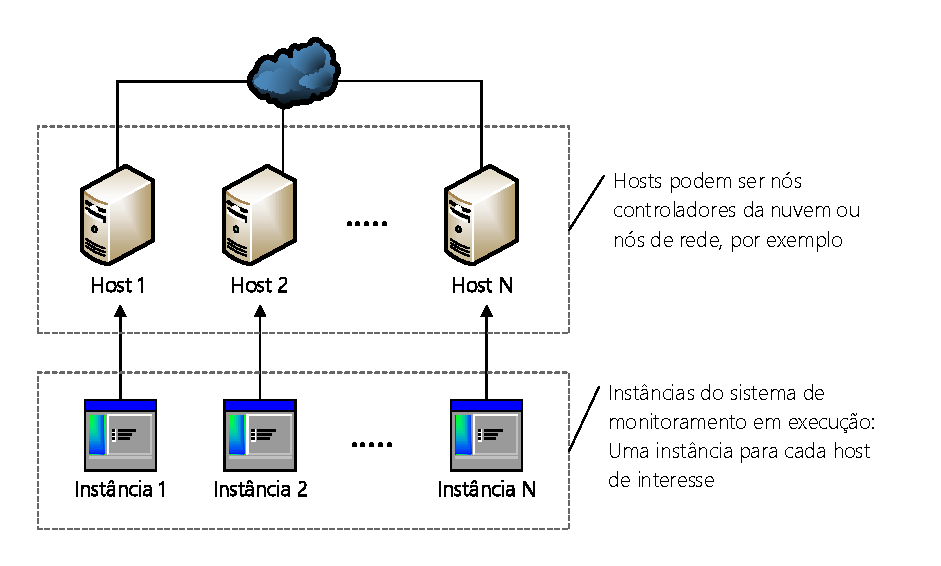
\includegraphics[width=.9\textwidth]{img/arquitetura_instalacao.pdf}
	\label{fig:proposta_instalacao}\\
    \vspace{-0.3cm}
	Fonte: O próprio autor.
\end{figure}

Apesar de nem todos os hosts hospedarem \acp{api} dos serviços (F2) ou o RabbitMQ (F3), pode haver interesse em monitorar tal host caso o tráfego de controle de algum serviço de interesse origine ou vá para ele (F1).
%
A decisão se o pacote está relacionado com algum serviço de interesse é baseada na porta de destino, seguindo as portas por padrão na Tabela \ref{tab:openstack_service_list}.
%
Para realizar a coleta de tráfego, este sistema de monitoramento será desenvolvido em uma linguagem de alto nível que forneça métodos relacionados à biblioteca \texttt{libpcap}.
%
Esta biblioteca disponibiliza meios para sistemas UNIX capturarem tráfego em suas interfaces de rede, sendo elas virtuais ou físicas.
%
Das linguagens possíveis, a preferência é para Python, por dispor de diversas bibliotecas e funcionalidades que simplificam o desenvolvimento, mas podendo mudar caso desempenho torne-se um fator crítico, seguindo o requisito RNF2.

Abordando o comportamento do sistema em alto nível é possível abstrair comportamentos comuns às três funcionalidades, conforme ilustrado na Figura~\ref{fig:proposta_funcionamento}.
%
\begin{figure}[!htb]
	\centering
	\caption{Arquitetura do sistema de monitoramento em alto nível}
    \vspace{-0.5cm}
	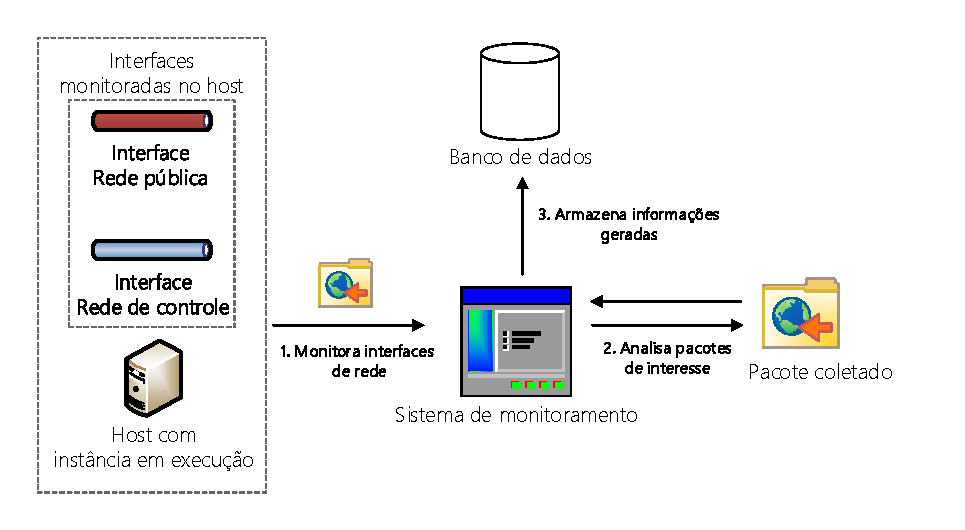
\includegraphics[width=1\textwidth]{img/arquitetura_funcionamento.pdf}
	\label{fig:proposta_funcionamento}\\
    \vspace{-0.6cm}
	Fonte: O próprio autor.
\end{figure}

\vspace{-0.3cm}
O sistema de monitoramento executará em um host de interesse, coletando tráfego nas interfaces de rede de acordo com as funcionalidades do sistema de monitoramento em execução naquele host, respeitando o requisito RNF1 (passo 1 na Figura \ref{fig:proposta_funcionamento}).
%
Caso um host não hospede \acp{api} de serviços, ou o \textit{middleware} de comunicação, por exemplo, é possível executar o sistema de monitoramento apenas para monitorar o tráfego na interface da rede de controle, pois é por onde passa o tráfego dos serviços de interesse, que é registrado pela F1.
%
Apesar de existirem outros níveis de agregação de tráfego, neste sistema de monitoramento é necessário realizar a medição a nível de pacote.
%
A agregação a nível de fluxo, por exemplo, apesar de popular, omite detalhes relevantes para este sistema de monitoramento, como o conteúdo do pacote.
%
Outro motivo é que apenas um pacote pode ser o suficiente para provocar mudanças no comportamento da nuvem, tal como uma requisição de criação de instância.
%
A agregação de tráfego com uma granularidade mais grossa perde tais detalhes, que devem ser levados em consideração no monitoramento, de acordo com o requisito RF4.

Os pacotes coletados são filtrados conforme a funcionalidade em execução no sistema de monitoramento daquele host, que nos três casos verificam a porta de destino (passo 2 na Figura \ref{fig:proposta_funcionamento}).
%
Na F1, qualquer pacote que tenha a porta de destino pertencente a uma das portas contida na Tabela \ref{tab:openstack_service_list}, por padrão, será aceito.
%
Em relação à F2, apenas pacotes destinados às portas na qual as \acp{api} executam serão aceitos.
%
Para a F3, os pacotes destinados à porta na qual o RabbitMQ executa serão aceitos.
%
Após, cada funcionalidade realiza seu processamento utilizado informações extraídas dos pacotes filtrados, posteriormente gravando no banco de dados escolhido, que é acessado por todas as instâncias em execução para gravar as informações geradas (passo 3 na Figura \ref{fig:proposta_funcionamento}).
%
Em relação aos dados armazenados, cada funcionalidade terá sua própria estrutura de armazenamento no banco de dados, que no caso de banco de dados relacionais (\textit{i.e.,} MySQL, PostgreSQL), é o equivalente a uma ou mais tabelas para cada funcionalidade.
%
O restante desta seção detalhará o funcionamento das três funcionalidades de monitoramento, na qual F2 e F3 serão agrupadas na explicação por conta da sua semelhança no funcionamento.

\subsection{F1: Classificação consumo de banda, rede de controle}
% @TODO -> parei revisão 1 aqui
Esta funcionalidade tem como objetivo auxiliar na análise longitudinal de tráfego na rede de controle.
%
Contudo, será considerado apenas o tráfego gerado pelos serviços delimitados na Tabela~\ref{tab:openstack_service_list} para simplificar o escopo deste TCC.
%
O diagrama de sequência na Figura \ref{fig:proposta_sequencia_servicos} ilustra os passos de funcionamento desta funcionalidade do sistema de monitoramento.

\begin{figure}[!htb]
	\centering
	\caption{Diagrama de sequência: monitoramento de banda consumida pelos serviços}
    \vspace{-0.3cm}
	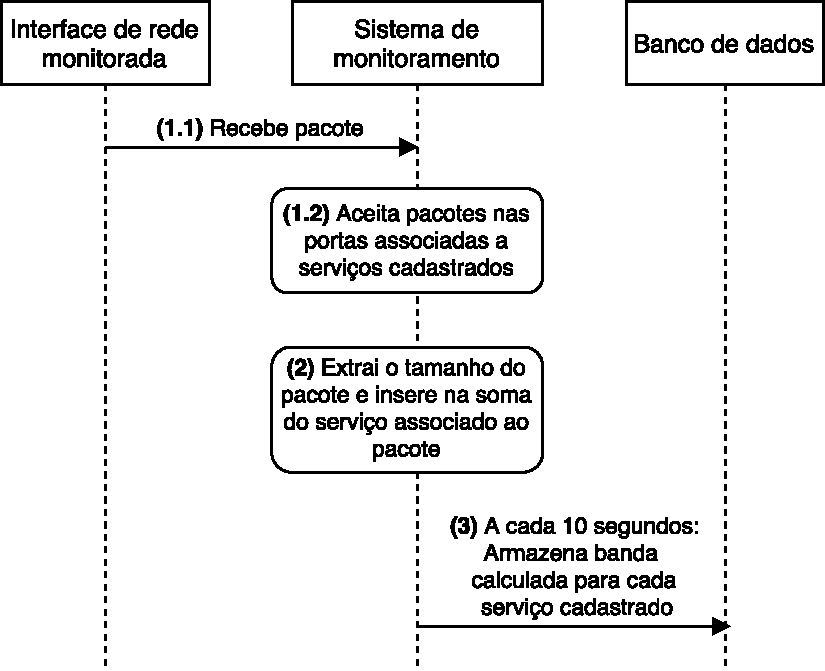
\includegraphics[width=0.77\textwidth]{img/sequencia_monitoramentoServicos.pdf}
	\label{fig:proposta_sequencia_servicos}\\
%    \vspace{-0.3cm}
	Fonte: O próprio autor.
\end{figure}

Os passos que esta funcionalidade executa são:

\begin{enumerate}
\item Esta funcionalidade monitora apenas a interface da rede de controle, buscando todo tráfego que tenha como destino uma das portas associadas aos serviços em execução naquele host.
%
As portas também são utilizadas para criar uma classificação de serviços, cuja porta de destino serve para decidir em qual serviço aquele pacote está associado;

\item Após definido o serviço destino daquele pacote, é extraído o tamanho daquele pacote, que é somado a um contador de tráfego para aquele serviço.
%
Assim, por exemplo, todos os pacotes recebidos por certo serviço ao longo de um tempo têm seu tamanho somado, e então esta soma é dividida pelo período de tempo estabelecido (\textit{e.g.,} 5s, 10s).
%
Ou seja, ao somar todo o tráfego recebido ao longo de um período, e depois dividir esta soma pelo período, é possível estabelecer uma aproximação da quantidade de banda utilizada (em KB/s) para o serviço em questão naquele período.
%
Esta técnica é feita para todos os serviços considerados nesta análise, cada qual tendo seu próprio contador; e

\item Para cada uma destas somas é feita uma entrada no banco de dados, contendo o serviço e o cálculo de banda usada pelo serviço.
%
No caso de oito serviços monitorados com um período de 10s, por exemplo, a cada 10s serão realizadas oito inserções, em que cada uma contém a quantidade de banda destinada ao seu serviço naqueles 10s.
%
Após realizada a inserção o contador de cada serviço volta para zero, e faz o processo de inserção no banco de dados após 10s novamente.
\end{enumerate}


\subsection{F2 e F3: Cadastrar eventos detectados na \ac{api} dos serviços e no \textit{middleware} de comunicação}

Ambas F2 e F3 comportam-se de maneira similar, variando apenas a porta de destino observada e o conteúdo/protocolo dos pacotes analisados.
%
A Figura~\ref{fig:proposta_sequencia_transacao} ilustra um diagrama de sequência para F3, que monitora as transações internas da nuvem passando pelo \textit{middleware} de comunicação.
%
Para gerar informações significativas deve-se relacionar os dados gerados por estas funcionalidades com outras, sendo possível relacionar as duas, por exemplo, e criar uma sequência detalhada de ações na nuvem a partir de uma requisição, conforme feito por \citeonline{sharma:2015:hansel}.

\begin{figure}[!htb]
	\centering
	\caption{Diagrama de sequência: monitoramento de transações internas da nuvem}
	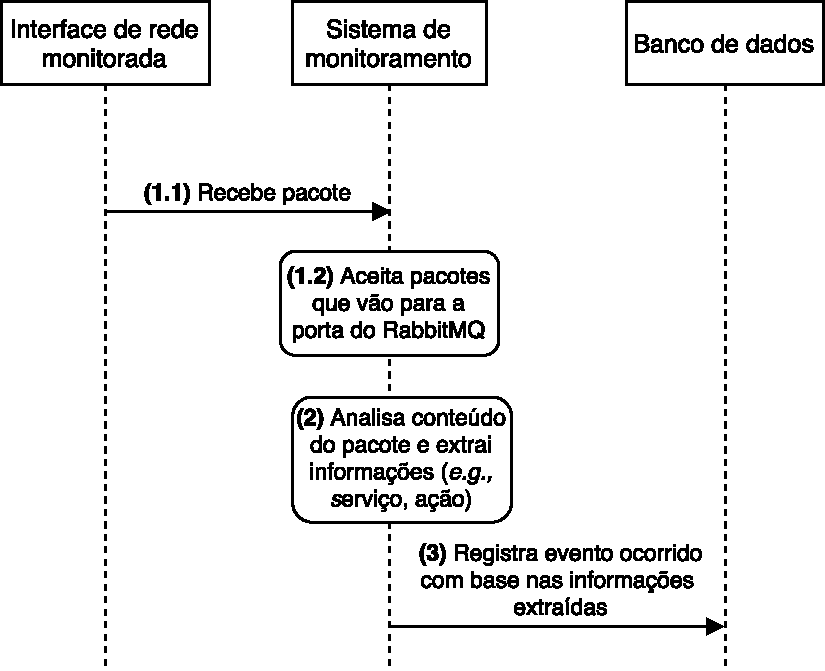
\includegraphics[width=0.78\textwidth]{img/sequencia_monitoramentoTarefas.pdf}
	\label{fig:proposta_sequencia_transacao}\\
	Fonte: O próprio autor.
\end{figure}

As ações nestas funcionalidades ocorrem da seguinte forma, tomando o diagrama de sequência da F3 (Figura \ref{fig:proposta_sequencia_transacao}) como base:

\begin{enumerate}
\item A F2 monitora a interface da rede pública, enquanto a F3 monitora a interface da rede de controle.
%
Ao receber pacotes, ambas as funcionalidades olham na porta de destino para decidir se aceitam os pacotes, na qual a F2 verifica se a porta de destino é de uma \ac{api} que o host hospeda; e no caso da F3, é verificado se a porta de destino é a mesma que a do \textit{middleware} de comunicação que o host hospeda; e

\item A princípio ambas as funcionalidades armazenarão as mesmas informações, mesmo que os protocolos de comunicação analisados sejam diferentes (HTTP na F2, e \ac{rpc} na F3).
%
Ou seja, para ambos as principais informações a armazenar são: serviço de origem, serviço de destino, IP do host e identificador da ação;

\item Por fim, armazena-se os dados de cada funcionalidade em suas respectivas tabelas.
\end{enumerate}


Conforme definido, através da implementação deste sistema de monitoramento será possível gerar os dados necessários para realizar a caracterização de tráfego proposta para a rede de controle.
%
A F1 é capaz de gerar informações relevantes em tempo real, possibilitando, por exemplo, verificar a variação do uso de banda pelos serviços ao longo de um período determinado.
%
Diferentemente, as funcionalidades F2 e F3 geram dados que necessitam de uma análise mais minuciosa, realizada na etapa posterior à coleta, especificada na Seção \ref{cap3:analise}.


\section{Análise de tráfego}
\label{cap3:analise}

A etapa de análise de tráfego, que será aplicada nos dados gerados pelo sistema de monitoramento (definido na Seção \ref{cap3:monitoramento}) busca gerar informações que ajudem a compreender melhor o comportamento do tráfego analisado.
%
Esta análise terá escopo limitado, no sentido de considerar apenas os serviços contidos na implementação mais popular de nuvem OpenStack, segundo \citeonline{openstack:newton}: Nova, Neutron, Cinder, Swift, Keystone e Glance.
%
A proposta atual pretende caracterizar três ângulos diferentes na rede de controle:

\begin{itemize}
	\item \textbf{Caracterização de funcionalidades da nuvem:} Busca entender como a execução de tarefas pelo consumidor influencia no funcionamento da rede de Controle da nuvem. 
	%
	A proposta inicial tem foco no ciclo de vida de \acp{vm} do OpenStack (\textit{e.g.,} criação de \ac{vm}, iniciação de \ac{vm}, pausar \ac{vm} em execução).
	
	\item \textbf{Consumo de banda por serviços:} Esta análise longitudinal tem como objetivo entender quais dos serviços considerados na análise mais geram tráfego na rede de Controle.
	
	\item \textbf{Influência de eventos periódicos no comportamento da nuvem:} Listar alguns dos eventos periódicos gerados pelos serviços da nuvem, e verificar qual o impacto gerado por eles na rede de controle. 
\end{itemize}

A \textbf{caracterização de funcionalidades da nuvem} utilizará informações geradas pelas F2 e F3, definidas no sistema de monitoramento.
%
Estas funcionalidades geram dados referentes à comunicação com as \acp{api} da nuvem, e da comunicação interna dos serviços, feita através do RabbitMQ.
%
Sendo assim, é possível criar uma sequência que mostra a trajetória do tráfego durante a realização de uma tarefa na nuvem a partir de uma requisição recebida pela \ac{api}.
%
Ou seja, a partir de uma requisição de um consumidor (\textit{e.g., } criação de \ac{vm}), cria-se um grafo direcionado que mostra quais mensagens foram enviadas para quais serviços à fim de concretizar a tarefa em questão.
%
Segundo \cite{sharma:2015:hansel} é possível gerar esta sequência de eventos, mas ainda não foi realizada uma análise profunda para verificar se realmente existe alguma variável que pode ser utilizada para interligar estas mensagens diretamente.

A análise de \textbf{consumo de banda por serviços} baseia-se na F1 do sistema de monitoramento, que contabiliza o tráfego gerado por cada um dos serviços considerados na análise.
%
A F1 do sistema de monitoramento deve gerar dados que podem ser interpretados diretamente, possibilitando a realização desta análise em tempo real.
%
Sendo assim, é possível por exemplo, acessar os dados gerados por esta funcionalidade definindo o período de início e de fim da análise, na qual gera um gráfico mostrando qual a porcentagem de tráfego destinado a cada serviço.

Por fim, a análise da \textbf{influência de eventos periódicos no comportamento da nuvem} deve se basear principalmente nos dados gerados pela F1 do sistema de monitoramento, na qual buscará grandes variações no recebimento de tráfego dos serviços em curtos períodos de tempo.
%
Baseando-se nestas variações serão consultados os dados gerados pelas F2 e F3 naquele período, que constará quais serviços enviaram as mensagens em questão.
%
Ou seja, como produto final este ângulo de caracterização busca mostrar quem executou aquele evento periódico, qual a tarefa em questão, e se há impacto significativo.
%
Definida a abordagem utilizada para a realização da caracterização de tráfego, o passo final é explicar como será realizado o experimento que aplicará a proposta definida neste capítulo.


\section{Plano de testes}
\label{cap3:experimento}

O plano de testes visa definir os experimentos a serem executados, os quais aplicarão a proposta de caracterização de tráfego.
%
A finalidade destes experimentos é validar o sistema de monitoramento desenvolvido e a abordagem para análise do tráfego.
%
No total serão realizados três experimentos, divididos em dois cenários diferentes, sendo que dois experimentos serão realizados em um dos cenários, e o outro cenário será usado no experimento restante.

\begin{itemize}
\item \textbf{Cenário 1:} Uma nuvem OpenStack com ambiente controlado, na qual toda interação com ela será originária dos experimentos executados; e

\item \textbf{Cenário 2:} Uma nuvem OpenStack em ambiente de produção, com consumidores utilizando-a.
\end{itemize}

Os experimentos visam verificar o funcionamento do sistema de monitoramento, e então analisar os dados gerados após a execução. 
%
Estes experimentos são:

\iffalse
\begin{itemize}
	\item \textbf{Experimento 1:} Visa verificar o funcionamento da função do sistema de monitoramento responsável por registrar o consumo de banda na rede de controle dos serviços do OpenStack, que será realizado no \textbf{cenário 1}.
    %
    O sistema de monitoramento executará apenas a função responsável por registrar o consumo de banda dos serviços, na qual o período de monitoramento será de um dia.
    %
    Durante este período, a nuvem em questão não receberá qualquer requisição originária de consumidor, e não hospedará nenhuma \ac{vm} em execução.
    %
    Os dados de consumo de banda gerados neste experimento serão armazenados e analisados, com o objetivo de estabelecer uma linha base de consumo de banda em nuvens OpenStack.
\end{itemize}
\fi

\begin{itemize}
	\item \textbf{Experimento 1:} Verificar o funcionamento do sistema de monitoramento, com o objetivo de avaliar a quantidade de dados gerados no monitoramento do \textbf{Cenário 1}.
    %
    O sistema de monitoramento utilizará todos as suas funcionalidades, na qual instâncias executarão em todos os hosts de interesse por um período de sete dias.
    %
    Durante este período, a nuvem deverá receber algumas requisições, que simularão atividades de consumidores, mas de forma esporádica.
    %
    Deste modo, será avaliada a quantidade de dados gerados, com o objetivo de verificar, por exemplo, se o banco de dados utilizado é adequado no caso de monitorar uma nuvem em ambiente de produção.
\end{itemize}

\begin{itemize}
	\item \textbf{Experimento 2:} Análise longitudinal do consumo de banda pelos serviços de uma nuvem em ambiente de produção (\textbf{Cenário 2}).
    %
    A função que registra o consumo de banda pelos serviços do OpenStack executará por um período de 30 dias.
    %
    Após, com os dados coletados será feita uma análise, com o objetivo de verificar a variação do consumo ao longo do período, identificando padrões de comportamento, por exemplo.
\end{itemize}

\begin{itemize}
	\item \textbf{Experimento 3:} Caracterização do comportamento da rede de controle em uma nuvem em ambiente de produção (\textbf{Cenário 2}).
    %
    O sistema de monitoramento utilizará todas as suas funcionalidades, na qual instâncias executarão em todos os hosts de interesse por um período de sete dias.
    %
    Ao longo deste período, a nuvem em questão será usada pelos consumidores e o sistema de monitoramento irá gerar dados sobre o uso.
    %
    Após, será feita uma caracterização de tráfego abordando dois ângulos de análise, definidos na Seção \ref{cap3:analise}: influência de eventos periódicos no comportamento da nuvem, e caracterização de funcionalidades da nuvem.
\end{itemize}

	Como comparativo, serão avaliados o tamanho do banco de dados nos experimentos 1 e 3, e verificar se há grande mudança na quantidade de dados gerados a partir do monitoramento.
    %
    Ambos os cenários utilizarão uma instalação similar do OpenStack, na qual os serviços caracterizados serão os mesmos.
    
    
\section{Considerações do Capítulo}
\label{cap3:consideracoes}

Este capítulo apresentou a proposta de caracterização de tráfego para uma nuvem computacional OpenStack.
%
A proposta baseia-se na análise da arquitetura de funcionamento de alguns serviços do OpenStack, o que possibilitou a definição de estratégias para utilizar no sistema de monitoramento, responsável pela primeira etapa: a medição de tráfego.
%
Foram definidos requisitos para a criação deste sistema de monitoramento, que abordam suas funcionalidades, e também pré requisitos, que devem ser considerados na construção dele.
%
O sistema de monitoramento em questão terá três funcionalidades que irão medir o tráfego e popular um banco de dados com as informações geradas a partir do tráfego avaliado.
%
Então, a etapa posterior, de análise de tráfego utilizará estas informações para melhor entender o comportamento da rede de controle sobre três ângulos de análise diferentes.
%
Após definir o que deve ser feito, a especificação do plano de testes determinou quais os experimentos que serão realizados, e também estabeleceu os cenários empregados nos experimentos.
\chapter{Proposta para análise de arquiteturas \ac{mmorpg}}
\label{cap3}



As arquiteturas de serviços \ac{mmorpg} são desenvolvidas visando suprir as necessidades do projeto do jogo desenvolvido, de forma a viabilizar a utilização deste serviço.
%
Nesse sentido, jogos com mecânicas de projeto similares possuem implementações parecidas para os clientes.
%
Entretanto, a arquitetura escolhida impacta no custo de operação e qualidade do serviço aos jogadores.
%
Por este motivo, diferentes arquiteturas com o mesmo \textit{design} não são comparáveis entre sí, visto que dependem das regras de negócio do jogo.



Ao desenvolver um serviço \ac{mmorpg} é necessário decidir uma arquitetura que possibilite reduzir custos, consumo de recursos e minimize ocorrências para os jogadores a fim de viabilizar a sua implantação como produto.
%
Porém, a impossibilidade de comparação direta entre as arquiteturas de serviço \ac{mmorpg} instiga a análise das características básicas destas arquiteturas que possam influenciar o \textit{game design}, tais como consumo de recursos, tempo de resposta, latência e número máximo de clientes simultâneos conectados nos microsserviços.
%
Sendo assim, uma análise do consumo de recursos computacionais das arquiteturas levantadas previamente na literatura tem valor científico no auxílio da escolha de implementações de arquiteturas de microsserviços, em específico para serviços \ac{mmorpg}.



Neste capítulo é descrita a proposta para análise de consumo de recursos computacionais em arquiteturas \ac{mmorpg}.
%
Inicialmente, é descrita a proposta em alto nível (Seção~\ref{sec:proposta}), trazendo os objetivos desta análise, quais recursos e métricas serão analisadas (TCC-II).
%
Os Critérios de Análise (Seção~\ref{sec:criterios}) exibem como os dados obtidos devem ser interpretados, baseando-se nos objetivos da análise das arquiteturas.
%
O Plano de Testes (Seção~\ref{sec:plano}) exibe como será realizada a coleta dos dados, descrevendo o ambiente, cenário, critérios e os testes que serão realizados. %para obter os objetivos deste trabalho.
%

\section{Proposta}
\label{sec:proposta}

Tendo analisado os trabalhos relacionados (Seção~\ref{sec:similares}) e as arquiteturas específicas para jogos \ac{mmorpg}, o presente trabalho tem como objetivo analisar as arquiteturas \ac{mmorpg} visando complementar a análise de arquitetura e consumo de recursos computacionais não analisados nos trabalhos relacionados.
%
Em específico, serão obtidos os valores referentes aos uso dos seguintes recursos computacionais nas arquiteturas Rudy (Subseção~\ref{rudy}), Salz (Subseção~\ref{salz}) e Willson (Subseção~\ref{willson}):

\begin{enumerate}
  \item \textbf{\ac{cpu}}: o uso de CPU, com sua representação sendo em relação a porcentagem de processamento nos núcleos utilizados;
  \item \textbf{Memória}: Quantidade de memória utilizada pelos processos do serviço/arquitetura. A sua representação será como dado absoluto;
  \item \textbf{Rede}: Banda de rede utilizada nas operações de entrada e saída para cada microsserviço, utilizando valores absolutos. Juntamente será obtido o valor de latência do cliente ao microsserviço, verificando se o congestionamento da rede afeta a latência do microsserviço.
\end{enumerate}

Além dos recursos computacionais, esta análise levará em conta valores referentes a outras métricas.
%
As métricas, cujos os valores serão obtidos são:

\begin{enumerate}
  \item \textbf{Número máximo de jogadores simultâneos}: Descobrir o limite de conexões para as arquiteturas propostas a análise. Será representado como valor absoluto.
  \item \textbf{Tempo de resposta das requisições}: Descobrir o tempo de resposta por categoria de requisição, conforme o número de jogadores no serviço. Será representado como tempo decorrido, em milissegundos.
\end{enumerate}

Todos estes valores serão obtidos a partir de simulações, e por este motivo faz-se necessário descrever o comportamento dos jogadores simulados (Seção~\ref{sec:SimulaCliente}).
%
Espera-se, em situações adversas, caracterizar os comportamentos das arquiteturas bem como gargalos e os custos de recursos computacionais para manutenção das arquiteturas de microsserviços.
%
Para este fim, faz-se necessário a descrição dos critérios que serão utilizados durante a análise dos valores obtidos nos experimentos.

\section{Critérios de análise}
\label{sec:criterios}

A fim de padronizar a análise dos dados obtidos, estes serão estabelecidos usando como base o comportamento dos valores obtidos em referenciais.
%
Neste sentido, a análise dos dados obtidos será guiada pelo esperado dos valores obtidos em um serviço padrão:

\begin{enumerate}
  \item \textbf{Consumo CPU}: Espera-se estressar com um elevado número de requisições.
  \item \textbf{Consumo Memória}: Espera-se estressar com requisições nas quais exija armazenamento em memória.
  \item \textbf{Vazão Rede - Entrada}: Espera-se estressar com requisições nas quais tenham uma carga de dados elevada.
  \item \textbf{Vazão Rede - Saída}: Espera-se estressar com respostas nas quais tenham uma carga de dados elevada.
  \item \textbf{Número de Conexões Simultâneas}: Servirá como guia de comparação com os demais valores e desempenho da arquitetura;
  \item \textbf{Tempo de resposta das requisições}: Servirá como guia de desempenho da arquitetura; e
  \item \textbf{Latência entre cliente e serviço}: Servirá como guia de comparação com os demais valores.
\end{enumerate}

Em um caso de uso ideal, todos os recursos não são estressáveis, com um número de conexões simultâneas elevado.
%
Porém, espera-se para este trabalho um possível conjunto de ocorrências, na qual podem ou não ocorrer.
%
Este conjunto servirá de guia / exemplo de problemas relevantes retirado dos valores obtidos.
%
Logo, a simulação e cenários foram elaborados para forçar tais ocorrências.


A partir dos valores obtidos, e seguindo o esperado de uma arquitetura totalmente relacionada ao número de conexões, espera-se encontrar um conjunto de eventuais problemas nas arquiteturas.
%
Um conjunto exemplo destes problemas estão listados na Tabela~\ref{tab:problemas}.
\pagebreak

\begin{table}[htb!]
  \centering
  \caption{Possíveis conjuntos para a análise.}
  \label{tab:problemas}
  \begin{tabular}{|l|l|l|l|l|l|l|l|}
  \hline
  \multicolumn{7}{|c|}{Recursos}                                                                      & \multirow{2}{*}{Descrição} \\ \cline{1-7}
  \rotatebox[origin=c]{90}{\ac{cpu}} & \rotatebox[origin=c]{90}{Memória} & \rotatebox[origin=c]{90}{Rede Entrada} & \rotatebox[origin=c]{90}{Rede Saída} & \rotatebox[origin=c]{90}{Conexões Simultâneas} & \rotatebox[origin=c]{90}{Tempo de Resposta} & \rotatebox[origin=c]{90}{Latência} &                            \\ \hline
  $\uparrow$    &              &              &              & $\downarrow$ &              &              & \thead{Rotina de processamento de requisições\\está ocupando muita \ac{cpu}} \\ \hline
                & $\uparrow$   &              &              & $\downarrow$ &              &              & \thead{O microsserviço está armazenando\\informações as quais poderiam estar alocadas em outros\\microsserviços}  \\ \hline
                &              & $\uparrow$   &              & $\downarrow$ &              &              & \thead{Uma entrada de dados elevada pode indicar\\o uso de um protocolo\\inapropriado para o serviço} \\ \hline
                &              &              & $\uparrow$   & $\downarrow$ &              &              & \thead{Caso a saída esteja muito elevada\\pode indicar uma configuração inapropriada de elementos\\que são transitados na rede ou\\uso inadequado de protocolos} \\ \hline
                &              &              &              & $\downarrow$ & $\uparrow$   &              & \thead{Pode estar relacionado\\ao desempenho de processamento,\\ modelo de paralelismo ou congestionamento de rede} \\ \hline
                &              &              &              & $\downarrow$ & $\uparrow$   & $\uparrow$   & \thead{Está relacionado com\\ congestionamento da rede} \\ \hline
  $\downarrow$  &              & $\uparrow$   & $\uparrow$   &              &              &              & \thead{Possível gargalo na rede\\ou protocolo ineficiente} \\ \hline
  $\uparrow$    & $\uparrow$   & $\downarrow$ & $\downarrow$ &              &              &              & \thead{Possível gargalo nos algoritmos\\utilizados no serviço} \\ \hline
                &              &              &              & $\downarrow$ &              &              & \thead{Bloqueio de novas conexões pelo\\sistema operacional ou\\modelo de paralelismo} \\ \hline
  $\uparrow$    & $\uparrow$   & $\uparrow$   & $\uparrow$   & $\uparrow$   & $\downarrow$ &  $\uparrow$  & \thead{Limite de processamento da arquitetura} \\ \hline
  $\downarrow$  & $\downarrow$ & $\downarrow$ & $\downarrow$ & $\uparrow$   & $\downarrow$ &  $\downarrow$& \thead{Teste ideal} \\ \hline


  \end{tabular}

  Fonte: O próprio autor.
\end{table}


Não foram encontrados trabalhos para guiar a caracterização dos dados, sendo assim a caracterização foi definida genericamente.
%
Dessa forma, a linha de base para a caracterização será encontrada ao decorrer da análise, utilizando dos valores de testes com poucas conexões (nenhum cliente e um cliente), esperando que o serviço escale linearmente conforme o inicio do processo.
%
A linha de base definida será uma das contribuições para trabalhos futuros.


A Tabela~\ref{tab:problemas} relaciona os recursos conforme dois padrões:

\begin{itemize}
  \item Valores acima da média ($\uparrow$).
  \item Valores baixo da média ($\downarrow$).
\end{itemize}

Espera-se encontrar problemas mais detalhados, além de problemas padronizados de forma genérica na Tabela~\ref{tab:problemas}.
%
Pode ser possível identificar eventuais problemas conforme o tipo de requisição e projeto da arquitetura.
%
Estes problemas servirão como guias na análise final das arquiteturas.

Seguindo estes critérios de análise, torna-se necessário definir um plano de testes a fim de obter os dados conforme os cenários e casos de uso definidos no atual trabalho.
%
Tais testes servem para ocasionar situações nos serviços a fim de obter dados para posterior análise.



\section {Plano de testes}
\label{sec:plano}



O plano de testes define os cenários que serão aplicados sobre as arquiteturas de microsserviços para jogos \ac{mmorpg} selecionadas.
%
Esta seção serve para descrever formas de estressar as arquiteturas, a fim de obter valores para análise.
%
Entretanto, antes de relatar os cenários de teste, é importante descrever o ambiente no qual serão realizados os experimentos.
%
A Figura~\ref{Ambiente de testes} descreve a infraestrutura utilizada para execução das camadas de aplicação utilizadas nos testes.



\begin{figure}[htb!]
  \caption{Ambiente de testes definido para a coleta de dados.}
  \label{Ambiente de testes}
  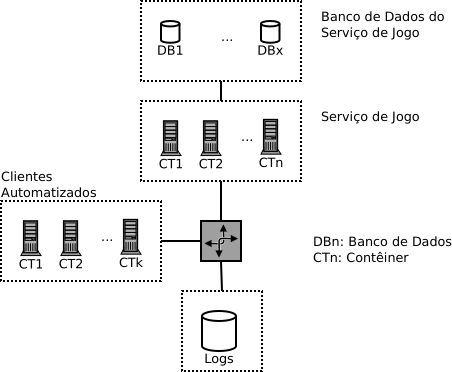
\includegraphics[width=0.8\textwidth]{img/cap3/infraestrutura.png}
  \centering

  Fonte: O próprio autor.
\end{figure}



Como visível na Figura~\ref{Ambiente de testes}, o ambiente de testes planejado está organizado em cinco regiões.
%
Essas regiões foram isoladas com o objetivo de diminuir o impacto de desempenho e consumo de recursos por outras ferramentas durante a coleta de dados.
%
Por este motivo, as regiões da infraestrutura planejada são:



\begin{enumerate}
  \item \textbf{Serviço de Jogo}: A camada de serviço da infraestrutura dos testes concentrará a arquitetura dos microsserviços referente às arquiteturas de microsserviços analisadas.
  \item \textbf{Banco de dados do serviço de jogo}: A camada de banco de dados do serviço de jogo conterá os serviços de dados e web a fim de manter um padrão de banco de dados para ambos os serviços utilizados e auxiliar na inicialização dos testes.
  \item \textbf{Estresse}: A camada de estresse será responsável por realizar requisições ao serviço a fim de estressá-lo, simulando padrões de requisição de um padrão de um jogador.
  \item \textbf{Cliente}: A camada de cliente será composta pelos mesmos elementos da camada de estresse, porém em um ambiente controlado para que a alta demanda dos clientes neste ambiente não interfira nas métricas obtidas.
  \item \textbf{Dados}: A camada de dados será composta por um banco de dados de \textit{log} a fim de armazenar os dados obtidos da camada Cliente e Serviço, posteriormente utilizado exclusivamente na coleta de dados.
\end{enumerate}



Tais regiões da infraestrutura utilizada no ambiente de testes devem manter um padrão ao qual seu propósito é garantir a inexistência de interferência entre os testes, focando em obter métricas válidas para posterior análise.
%
Dessa forma, espera-se dividir as aplicações conforme a sua rede, facilitando o seu monitoramento.
%
Entretanto, por se tratar de um sistema baseado em serviço, espera-se utilizar uma considerável parte do mesmo sistema de cliente para as três arquiteturas, excluindo-se os casos no quais a arquitetura necessite de alterações.




Para os casos de uso, serão utilizadas as arquiteturas de microsserviços específicos a jogos \ac{mmorpg} obtidos da literatura.
%
São essas elas:



\begin{enumerate}
  \item Arquitetura Rudy (Subseção~\ref{rudy}), na qual baseia-se na segregação de jogadores por canais;
  \item Arquitetura Salz (Subseção~\ref{salz}), na qual baseia-se em gerar muitos serviços escaláveis; e
  \item Arquitetura Willson (Subseção~\ref{willson}), na qual baseia-se em extrair microsserviços de regras de negócio mais custosas.
\end{enumerate}



Tais arquiteturas vão impactar o serviço de jogo, banco de dados e as requisições as quais os clientes deverão realizar.
%
Espera-se obter os valores referente a diferença de consumo de recursos computacionais dentro de cenários controlados utilizando o ambiente de testes.



Com o objetivo de obter dados, torna-se claro a necessidade de estresse das arquiteturas em múltiplos casos diversos, garantindo assim a confiabilidade dos dados obtidos.
%
Dessa forma, foi desenvolvido um cenário que comporte ambas as arquiteturas de microsserviços propostas na análise.
%
Este cenário possibilita a execução do experimento junto a simulação de clientes.



\subsection{Cenário}



O cenário reflete diretamente sobre o ambiente proposto para esta análise.
%
Este será executado sobre cinco camadas, nas quais cada camada estará isolada em sub-redes em uma nuvem de computadores.

O cenário será composto por cinco sub-redes, as quais cada uma será responsável pela operação de uma região do ambiente planejado (Figura~\ref{fig:cenario}).
%
Esta divisão física em redes facilitará a orquestração dos serviços na rede, seguindo boas práticas de implantação de microsserviços.
%
Além disso, pode-se garantir que a interface do serviço público para o cliente segue o padrão de um serviço \ac{mmorpg} real.

\begin{figure}[htb!]
  \caption{Rede de execução dos testes.}
  \label{fig:cenario}
  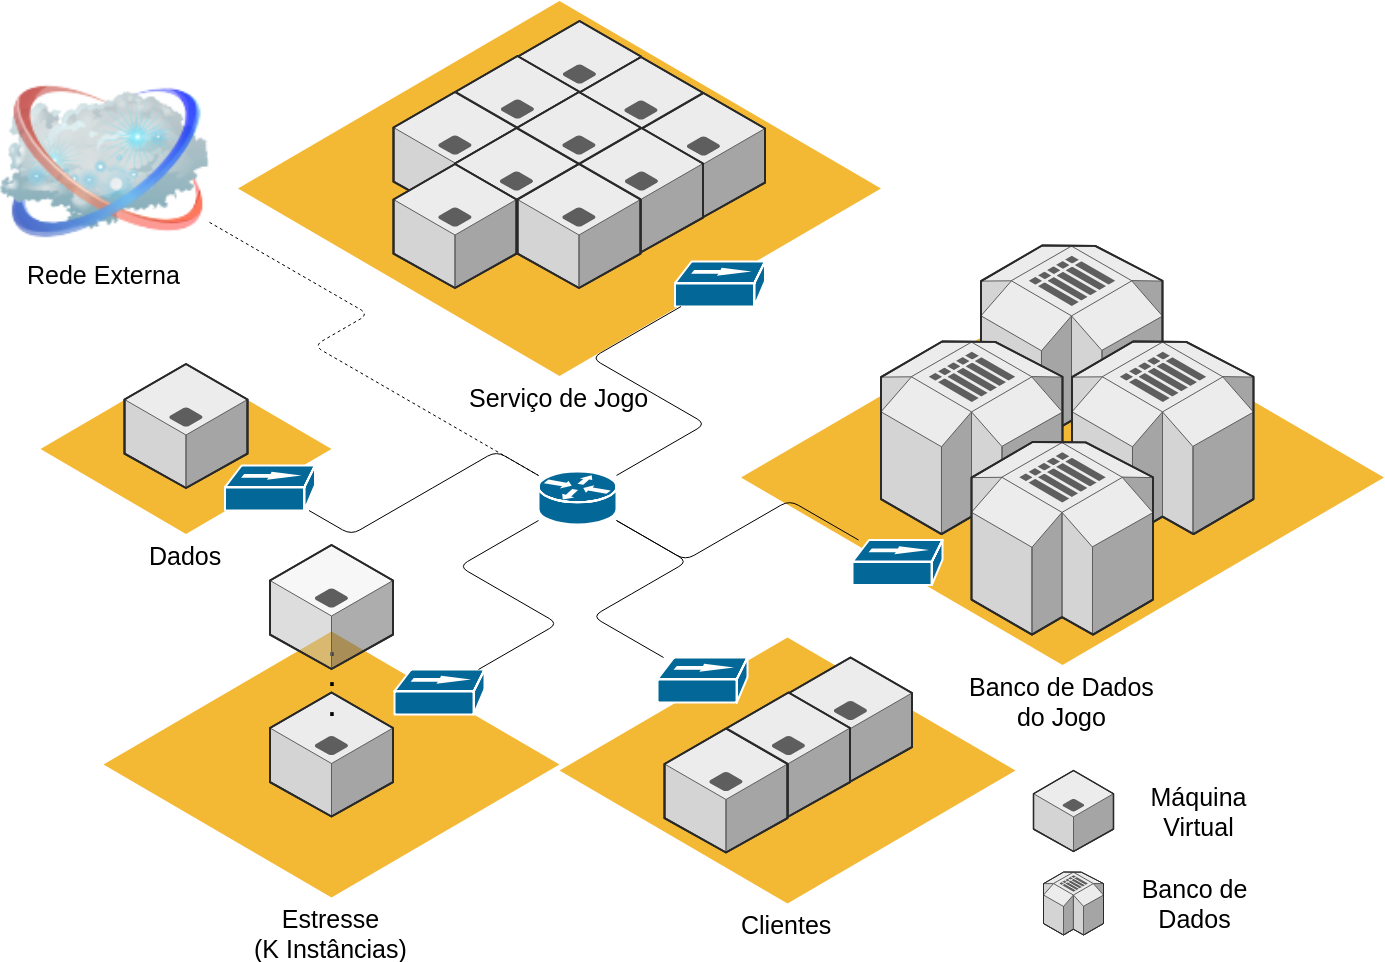
\includegraphics[width=\textwidth]{img/cap3/cenario.png}
  \centering

  Fonte: O próprio autor.
\end{figure}

O cenário, exibido na Figura~\ref{fig:cenario} descreve cinco sub-redes.
%
Estas redes são descritas da seguinte forma:

\begin{enumerate}
  \item \textbf{Dados}: Armazena e processa os dados obtidos da arquitetura. É usado pelas redes \textit{Cliente} e \textit{Serviço de Jogo}.
  \item \textbf{Banco de dados do serviço de jogo}: Armazena dados do jogo. É usado pela rede \textit{Serviço de Jogo}.
  \item \textbf{Serviço de Jogo}: Executa sistemas \textit{web} e \ac{rpc}, em específico da camada de serviço de jogo. Gera métricas para os serviços na rede \textit{Dados} e manipula os bancos de dados na rede \textit{Banco de dados do serviço de jogo}.
  \item \textbf{Estresse}: Executa múltiplos clientes, a fim de estressar o serviço de Jogo.
  \item \textbf{Clientes}: Executa um número controlado de clientes para obter métricas de tempo de resposta e latência entre as redes \textit{Cliente} e \textit{Serviço de Jogo}.
\end{enumerate}

Conforme a descrição de cada rede, existe uma interdependência dentre as redes.
%
Tal interdependência pode ser visualizada na Tabela~\ref{tab:interdependencia}.

\begin{table}[htb!]
\centering
\caption{Tabela de interdependência das sub-redes.}
\label{tab:interdependencia}
\begin{tabular}{|l|l|l|l|l|l|}
\hline
\multicolumn{1}{|c|}{\rotatebox[origin=c]{-45}{Linha depende de Coluna}}  & \rotatebox[origin=c]{90}{Dados} & \rotatebox[origin=c]{90}{Banco de dados do serviço de jogo} & \rotatebox[origin=c]{90}{Serviço de Jogo} & \rotatebox[origin=c]{90}{Estresse} & \rotatebox[origin=c]{90}{Clientes} \\ \hline
Dados                             & --    & Não                               & Não             & Não      & Não      \\ \hline
Banco de dados do serviço de jogo & Não   & --                                & Não             & Não      & Não      \\ \hline
Serviço de Jogo                   & Sim   & Sim                               & --              & Não      & Não      \\ \hline
Estresse                          & Não   & Não                               & Sim             & --       & Não      \\ \hline
Clientes                          & Sim   & Não                               & Sim             & Não      & --       \\ \hline
\end{tabular}

Fonte: O próprio autor.
\end{table}

A Tabela~\ref{tab:interdependencia} refere-se a dependência das redes, conforme os serviços necessários para o seu funcionamento.
%
Portanto, espera-se bloquear o tráfego de pacotes entre redes que são independentes.

A implantação do serviço de jogo utilizará métodos de implantação de microsserviços, com ferramentas para gerenciamento de nós em uma rede de contêineres.
%
Por este motivo, todas as máquinas virtuais da rede \textit{Serviço de Jogo} terão os mesmos recursos, facilitando o comportamento do gerenciador ao escalar os serviços.

A implantação dos bancos de dados do serviço de jogo devem ser implantadas diretamente no sistema operacional da máquina virtual.
%
Seguindo assim uma boa prática de não armazenar dados dentro de contêineres.
%
Por sua vez, estas máquinas virtuais serão focadas em armazenamento.

A implantação dos clientes sobre a rede \textit{Clientes} executará um número limitado de contêineres fixo sobre as máquinas virtuais, para que não estresse as instâncias desta rede.
%
Nesse sentido, os recursos computacionais requiridos por estas instâncias são menores em relação aos demais.

A estrutura de implantação da rede \textit{Estresse} será dada por um gerenciador de nós em uma rede de contêineres.
%
Esta rede terá mais instâncias sob demanda conforme o caso de teste.

O limite de recursos do cenário é definido na Tabela~\ref{tab:limite_recursos}, sendo definida a faixa de endereços de cada rede a qual foi projetada.
%
Estes valores podem ser alterados conforme a necessidade dos testes, tendo seus recursos reduzidos ou incrementados.

\begin{table}[htb!]
\centering
\begin{adjustbox}{max width=\textwidth}
\caption{Limite de recursos por instância de cada rede.}
\label{tab:limite_recursos}
\begin{tabular}{|l|l|l|l|l|l|}
\hline
Nome da Rede                      & Rede                     & Instâncias & Armazenamento / Ins. & N. Núcleos & Memória \\ \hline
Dados                             & 10.0.*.* / 255.255.0.0   & 1          & 250GB                & 4          & 4GB     \\ \hline
Banco de dados do serviço de jogo & 10.51.*.* / 255.255.0.0  & 4          & 100GB                & 4          & 2GB     \\ \hline
Serviço de Jogo                   & 10.52.*.* / 255.255.0.0  & 10         & 25GB                 & 4          & 4GB     \\ \hline
Estresse                          & 10.100.*.* / 255.255.0.0 & N          & 25GB                 & 4          & 4GB     \\ \hline
Clientes                          & 10.101.*.* / 255.255.0.0 & 3          & 10GB                 & 2          & 1GB     \\ \hline
\end{tabular}
\end{adjustbox}

Fonte: O próprio autor.
\end{table}

A partir da Tabela~\ref{tab:limite_recursos}, espera-se definir um limite de recursos máximos utilizados pelo Serviço de Jogo.
%
A única rede que pode variar conforme o teste será a rede Estresse, visto que a demanda para estressar uma rede pode mudar conforme as características do teste.

A partir deste cenário é definido qual o comportamento dos clientes na execução dos testes.
%
Nesse sentido, uma definição das características mínimas de regra de negócio, padrão de comportamentos e interface esperada para o serviço e cliente é necessária.



\subsection{Simulação de Clientes}
\label{sec:SimulaCliente}



Utilizando a simulação de clientes objetiva-se estressar as arquiteturas utilizando um ataque com \textit{bots}.
%
Neste cenário, para padronizar a coleta de dados, todos os \textit{bots} terão a mesma rotina evitando assim um comportamento aleatório, a qual pode descaracterizar os dados obtidos para análise.



Porém, como requisito para estipular as requisições, faz-se obrigatório realizar um levantamento de requisitos no qual tanto o serviço quanto o cliente devem implementar.
%
Nesse sentido, a Tabela~\ref{tab:requisitos_funcionais} relaciona a funcionalidade com o impacto de implementação de tal funcionalidade.



\begin{table}[htb!]
\centering
\begin{adjustbox}{max width=\textwidth}
\caption{Requisitos das funcionalidades e respectivo impacto de implementação.}
\label{tab:requisitos_funcionais}
\begin{tabular}{|l|l|l|}
\hline
Requisito                                                       & Descrição                                                                                                                                                                                  & Implementação                                                                                                                                                                             \\ \hline
Identificação                                                   & \begin{tabular}[c]{@{}l@{}}Gera uma numeração única (token) com base\\ em uma tupla de dados.\end{tabular}                                                                                 & \begin{tabular}[c]{@{}l@{}}Será implementado utilizando algoritmo de \textit{hash},\\ de forma a garantir que este token seja único e diferente a\\ cada implementação.\end{tabular}         \\ \hline
Autenticação                                                    & \begin{tabular}[c]{@{}l@{}}Recebe o token e garante que não existe nenhuma\\ conexão utilizando o mesmo token.\end{tabular}                                                                & \begin{tabular}[c]{@{}l@{}}Será implementado usando um serviço de chave valor,\\ como o Redis.\end{tabular}                                                                               \\ \hline
\begin{tabular}[c]{@{}l@{}}Seleção de\\ Personagem\end{tabular} & \begin{tabular}[c]{@{}l@{}}Uma conexão deve requerer o controle de um\\ personagem.\end{tabular}                                                                                           & \begin{tabular}[c]{@{}l@{}}Será implementado utilizando uma árvore de cena interna\\ ao serviço, onde o tipo do nó será Personagem e o seu nome\\ será o nome do personagem.\end{tabular} \\ \hline
Envio de Mensagem                                               & \begin{tabular}[c]{@{}l@{}}Será possível enviar mensagens e receber. Elas serão\\ baseadas na região. Será mantido uma distância fixa\\ para todos os casos de uso.\end{tabular}           & \begin{tabular}[c]{@{}l@{}}Deve existir uma estrutura de busca interna ao serviço para\\ consultar personagens de uma região em relação a um\\ usuário.\end{tabular}                      \\ \hline
Movimentação                                                    & \begin{tabular}[c]{@{}l@{}}Será possível movimentar o personagem para as\\ células adjacentes. Isso indica que o\\ posicionamento do personagem será baseado\\ em uma matriz.\end{tabular} & \begin{tabular}[c]{@{}l@{}}Esta ação deve comunicar a atualização para todos os demais\\ jogadores da região de interesse.\end{tabular}                                                   \\ \hline
Ataque                                                          & \begin{tabular}[c]{@{}l@{}}Ao atacar, o jogador causará um dano aleatório\\ baseado em seu nível em todos os inimigos das\\ células adjacentes.\end{tabular}                               & \begin{tabular}[c]{@{}l@{}}Esta ação irá manipular a árvore de objetos da cena do serviço\\ e deverá notificar todos os jogadores desta área de interesse.\end{tabular}                   \\ \hline
Consumo de Itens                                                & \begin{tabular}[c]{@{}l@{}}Ao consumir um item, os atributos do personagem\\ serão alterados, influenciando na regra de negócio\\ utilizada nas arquiteturas de teste.\end{tabular}         & \begin{tabular}[c]{@{}l@{}}Implicará na utilização de um banco de dados em memória\\ e manipulação de dados não visíveis pela\\ árvore de cena.\end{tabular}      \\ \hline
\end{tabular}
\end{adjustbox}

Fonte: O próprio autor.
\end{table}

A Tabela~\ref{tab:requisitos_funcionais} relata uma lista de funcionalidades mínimas que serão executadas na simulação.
%
A partir destas funcionalidades, pode-se definir quais requisições estarão disponíveis na \ac{api} para o cliente requisitar ao serviço.
%
A lista de comandos públicos é exibida na Tabela~\ref{tab:api_publica}.


\begin{table}[htb!]
\centering
\begin{adjustbox}{max width=\textwidth}
\caption{Requisitos mínimos funcionais para a implementação da simulação descrita.}
\label{tab:api_publica}
\begin{tabular}{|l|l|l|l|l|}
\hline
Nome                  & Argumentos            & Retorno & Protocolo & Direção              \\ \hline
\textit{Auth}                  & \textit{Username, Password}    & \ac{json} & \textit{Web}       & Cliente para Serviço \\ \hline
\textit{CreateAccount}         & \textit{Username, Password}    & \ac{json} & \textit{Web}       & Cliente para Serviço \\ \hline
\textit{UpdateAccount}         & \textit{Username, Password}    & \ac{json} & \textit{Web}       & Cliente para Serviço \\ \hline
\textit{CreateCharacter}       & \textit{Token, Character Name} & \ac{json} & \textit{Web}       & Cliente para Serviço \\ \hline
\textit{DeleteCharacter}       & \textit{Token, Character ID}   & \ac{json} & \textit{Web}       & Cliente para Serviço \\ \hline
\textit{SelectCharacter}       & \textit{Token, Character ID}   & \ac{json} & \ac{rpc}           & Cliente para Serviço \\ \hline
\textit{WalkTo}                & \textit{Token, PosX, PosY}     &           & \ac{rpc}           & Cliente para Serviço \\ \hline
\textit{ConsumeItem}           & \textit{Token, Item}           &           & \ac{rpc}           & Cliente para Serviço \\ \hline
\textit{AtackHere}             & \textit{Token}                 &           & \ac{rpc}           & Cliente para Serviço \\ \hline
\textit{SendMessage}           & \textit{Token, Message}        &           & \ac{rpc}           & Cliente para Serviço \\ \hline
\textit{UpdateMapEstate}       & \textit{NPC, Action, MoreData} &           & \ac{rpc}           & Serviço para Cliente \\ \hline
\textit{UpdateCharacterEstate} & \textit{NPC, Action, MoreData} &           & \ac{rpc}           & Serviço para Cliente \\ \hline
\textit{ReceiveMessage}        & \textit{NPC, Message}          &           & \ac{rpc}           & Serviço para Cliente \\ \hline
\textit{ReBind}                & \textit{IP, Port}              &           & \ac{rpc}           & Serviço para Cliente \\ \hline
\end{tabular}
\end{adjustbox}
\end{table}

A Tabela~\ref{tab:api_publica} descreve todos os comandos que estarão disponíveis na rede.
%
Além destes, serão implementados outros comandos para \ac{api} privada do serviço.
%
Porém, os demais comandos da \ac{api} privada não serão utilizados pelo cliente, sendo necessariamente um requisito para o funcionamento do serviço com determinada arquitetura.


O ambiente da simulação será baseado em matrizes.
%
Cada mapa pode ser visualizado como uma matriz de 100x100 unidades.
%
Dessa forma, temos um ambiente com valor exato, o qual facilita cálculos internos do serviço e cliente, assim promovendo um ambiente vasto porém sem utilizar recursos de forma exagerada para os testes.
%
Os personagens podem locomover-se para as células adjacentes a sua localização.
%
O raio de interesse é de quatro células.
%
Um exemplo de estado do ambiente do jogo pode ser visualizado na Figura~\ref{fig:roi}.

\begin{figure}[htb!]
  \caption{Área de interesse da simulação com raio de quatro células.}
  \label{fig:roi}
  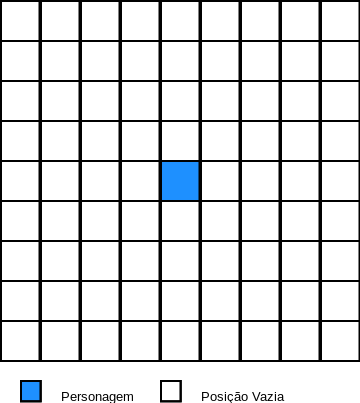
\includegraphics[height=8.0cm]{img/cap3/roi.png}
  \centering

  Fonte: O próprio autor.
\end{figure}

A partir da área de interesse do jogo, como o da Figura~\ref{fig:roi}, o \textit{bot} poderá decidir suas ações baseado em um autômato.
%
Caso ele alcance os extremos do mapa, ele será movimentado para outro mapa.
%
Nos casos de arquiteturas com múltiplos gerenciadores de mundo, será utilizado o comando \textit{ReBind} para realizar a conexão com o microsserviço correto após o translado do personagem.



Todas as ações do \textit{bot} no mapa são baseadas em um autômato.
%
Sendo assim, espera-se obter um padrão de movimentação a fim de evitar ciclos que um jogador comum dificilmente realizará (\textit{e.g.,} Andar para frente e para trás, ficar equipando itens em ciclo, ficar consumindo itens até acabar, \textit{etc.}).
%
A movimentação do personagem seguirá o autômato descrito na Figura~\ref{fig:movimentacao}.


\begin{figure}[htb!]
  \caption{Autômato de movimentação dos personagens simulados.}
  \label{fig:movimentacao}
  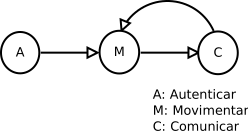
\includegraphics[height=5.5cm]{img/cap3/movimentacao.png}
  \centering

  Fonte: O próprio autor.
\end{figure}

A Figura~\ref{fig:movimentacao} descreve o comportamento de um \textit{bot} no ambiente do jogo simulado.
%
Ele seguirá um padrão de procurar batalhas, batalhar, gerenciar itens do personagem e buscar novas batalhas.
%
Este conjunto de ações simula o comportamento de busca de itens dentro de um jogo \ac{mmorpg}.
%
As características específicas de cada estado são definidas da seguinte forma:

\begin{itemize}
  \item Autenticar: Realizará autenticação com o serviço \textit{web} ou \textit{rpc} apropriado a arquitetura. Neste passo o \textit{bot} receberá as informações do seu personagem.
  \item Buscar Inimigo: Caminhará de forma aleatória a fim de buscar um inimigo, caso não exista em sua área de interesse. Caso encontre em sua área de interesse, irá aproximar deste inimigo.
  \item Batalhar: Irá atacar um inimigo, aplicando dano a este \ac{npc}. O personagem poderá receber dano. Estes valores serão fixos baseados em seu equipamento. O personagem pode perder todos os seus pontos de vida, sendo desconectado do serviço.
  \item Gerenciar Itens: O \textit{bot} irá consumir itens para recuperar pontos de vida e usar equipamentos melhores aos já utilizados.
  \item Caminhar Aleatoriamente: O personagem caminhará aleatoriamente por um número de passos máximo. Após isso, voltará a buscar uma batalha.
\end{itemize}

Esta sequência de ações visa forçar aos \textit{bots} a exploração do cenário.
%
A cada mudança de estado, o jogador irá anunciar no chat a sua troca de ação.
%
Isso contribuirá com o monitoramento do comportamento dos personagens tanto quanto usará a funcionalidade de chat.
%
Para simular a ação de resposta de mensagens de um jogador, cada \textit{bot} que receber uma mensagem terá uma porcentagem fixa de $25\%$ de probabilidade de responder a sua ação no atual momento.
%
Um \textit{bot} não poderá responder a uma mensagem na qual ele mesmo emitiu na região.


Ao realizar um \textit{ReBind} ou transitar de um mapa para o outro, o estado atual do autômato volta para o estado \textbf{Autenticar}.
%
Caso já esteja autenticado, continuará a sua busca por inimigos na nova região.

O ambiente final da simulação possui três mapas no eixo horizontal e no eixo vertical, visto que esta é a combinação mínima para que o serviço tenha um mapa central com bordas para efetuar transições de novos personagens.

Após definido as características dos clientes simulados, pode-se definir os testes que serão executados sobre as arquiteturas de microsserviços específicos para jogos \ac{mmorpg}.
%
Tais testes servem de guia para obter as métricas para a análise das arquiteturas de microsserviços especificadas.

\subsection{Testes}

Os testes que serão executados no atual trabalho esperam analisar a quantia de recursos mínimos para executar os microsserviços e o crescimento de consumo de recursos conforme o crescimento de clientes simultâneos.
%
Nesse sentido, foram definidos os seguintes testes:

\begin{enumerate}
  \item Executar as arquiteturas com zero jogadores simultâneos, por 5 minutos;
  \item Executar as arquiteturas com um jogador apenas; e
  \item Executar as arquiteturas com zero jogadores simultâneos, aumentando a cada minuto o número jogadores (\textit{e.g.,} 10) ao serviço, até o serviço obter algum erro interno de microsserviço e terminar a sua execução por erro interno.
\end{enumerate}

Os dados são capturados ao decorrer do tempo, podendo assim relacionar os recursos consumidos com o número de conexões simultâneas no serviço e com os demais recursos.
%
Esta estrutura auxiliará a visualização e interpretação dos dados para posterior análise.

Todos os testes serão executados utilizando a arquitetura Rudy, Salz e Willson.
%
Eles serão executados sequencialmente, aplicando sobre o cenário cada arquitetura e seus devidos clientes sobre o cenário, a fim de obter as métricas para posterior análise.
%
A partir desta sequência de testes, são obtidos valores suficientes para a análise das arquiteturas de microsserviços específicas a jogos \ac{mmorpg}.
%
Estes serão utilizados para análise conforme os critérios definidos na Seção~\ref{sec:criterios}, buscando possíveis gargalos e problemas de escalabilidade do sistema.


\section{Considerações parciais}


Este capítulo definiu os objetivos da análise de microsserviços específicos a jogos \ac{mmorpg}.
%
Para alcançar tais objetivos, se fez necessário definir quais métricas serão obtidas e como estes dados serão analisados.
%
Por fim, definiu-se qual o ambiente, cenário e testes que serão executados para obter tais dados.

Dessa forma, foi definido que será obtido os valores de uso de \ac{cpu}, memória, vazão de rede (tanto para entrada quanto saída), número de conexões simultâneas, tempo de resposta das requisições e latência entre cliente e serviço.
%
Estes valores serão analisados conforme possíveis problemas conhecidos, definidos na seção de critérios (Seção~\ref{sec:criterios}).

A fim de obter tais valores para análise, o plano de testes definiu um ambiente baseado em camadas conforme a demanda das arquiteturas submetidas a análise.
%
Foram projetadas cinco sub-redes no cenário de testes baseado nas regiões definidas no ambiente de testes.
%
A partir destas sub-redes, foi estipulado valores de recursos computacionais limites e números de instâncias máximas.
%
Entretanto, não foi possível definir o limite de instâncias para a sub-rede de estresse, visto que não foi encontrado estudos anteriores para ter uma linha base de consumo de recursos.
%
Dessa forma, o atual trabalho contribuirá conjuntamente com futuros trabalhos guiando o consumo de recursos para as arquiteturas Rudy, Salz e Willson.
%
Por fim, foram definidas as regras de negócio básicas para os clientes simulados, baseados em um autômato.

Os testes que serão executados sobre as redes estão baseados na finalidade de obtenção de valores de recursos mínimos para execução dos serviços e crescimento de valores de recursos conforme um número de clientes simultâneos.

 
\chapter{Desenvolvimento das arquiteturas propostas}
\label{cap5}
%ccm <-9

\section{Topologia da Rede}
\label{sec:topologia}

A topologia da rede seguiu o padrão proposto na Seção~\ref{cap3}.
%
O principal objetivo da topologia proposta é segregar as instâncias na camada de rede, evitando interferências do orquestrador de microsserviços que é utilizado na etapa de implantação, visto que a implantação dos clientes também é feita com um orquestrador de microsserviços para simplificar a execução dos experimentos.

A segregação em sub-redes é importante visto que, a fim de otimizar o transporte de dados entre os serviços, tais orquestradores trocam mensagens na rede utilizando memória quando a conexão é realizada para o próprio hospedeiro.
%
Segregando em sub-redes, o orquestrador é forçado a realizar a conexão com as instâncias externas utilizando a pilha completa dos protocolos \ac{tcp} e \ac{udp}, a qual são eventuais pontos de gargalo em tais arquiteturas.
%
Nesse sentido, espera-se que não exista troca de mensagens entre o cliente e serviço de jogo executando em memória.
%
Dessa forma, há a possibilidade de analisar eventuais gargalos na rede.

Para gerenciar as sub-redes da topologia, foi utilizado o gestor de sub-redes da Nuvem Tchê~\footnote{Nuvem Tche: \url{http://www.labp2d.joinville.udesc.br/}}, o qual é um serviço básico do sistema de gestor de nuvens computacionais OpenStack~\footnote{OpenStack: \url{https://www.openstack.org/}}.
%
O OpenStack permite acoplar interfaces de rede virtuais a instâncias computacionais selecionadas, a fim de conectá-las a uma sub-rede virtualizada.

Utilizando o gestor do OpenStack, foram definidas quatro sub-redes a fim de isolar a rede do banco de dados, rede do serviço de jogo, rede dos clientes e rede do serviço de métricas.
%
Esta topologia utilizada nos experimentos com as arquiteturas Rudy, Salz e Willson são ser exibidas na Figura~\ref{fig:topologia}.


\begin{figure}[htb!]
    \caption{Topologia da rede no gestor de redes do OpenStack.}
    \centering
    \begin{subfigure}{0.5\textwidth}
      \centering
      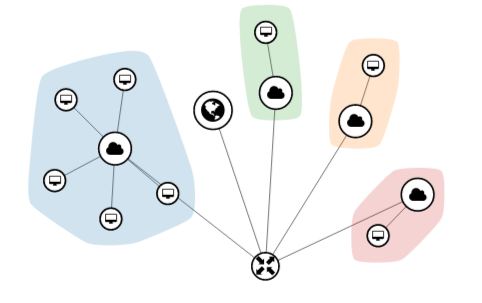
\includegraphics[width=.8\textwidth]{img/cap5/topology_graph.png}
      \caption{Grafo OpenStack do experimento.}
      \label{fig:topologia_a}
    \end{subfigure}%
    \begin{subfigure}{0.5\textwidth}
      \centering
      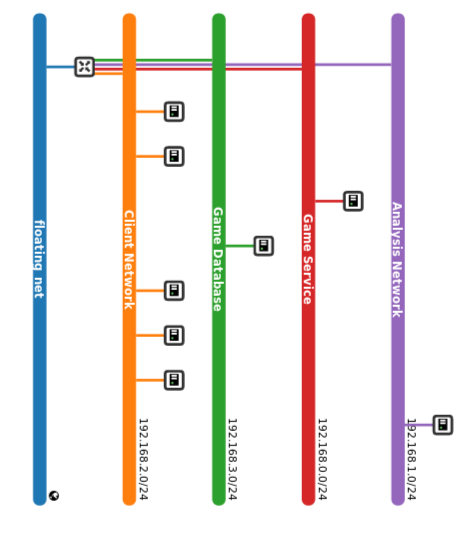
\includegraphics[width=.8\textwidth]{img/cap5/topology.png}
      \caption{Topologia da rede OpenStack.}
      \label{fig:topologia_b}
    \end{subfigure}
    \label{fig:topologia}

    Fonte: O próprio autor.
\end{figure}


A Figura~\ref{fig:topologia} mostra a disposição das instâncias em sub-redes exibindo-as como um grafo (Subfigura~\ref{fig:topologia_a}) e em forma de barramento (Subfigura~\ref{fig:topologia_b}).
%
A visualização em Grafo (Subfigura~\ref{fig:topologia_a}) ajuda a compreender a disposição das instâncias computacionais e a conectividade entre cada instância do ambiente de experimentos.
%
Já a visualização em barramento (Subfigura~\ref{fig:topologia_b}) exibe características técnicas como a faixa de \ac{ip} e nome das sub-redes.
%
Ambos os gráficos são complementares para informar as características básicas da interconexão das sub-redes.

A Figura~\ref{fig:topologia} também exibe oito instâncias utilizadas nos testes, na qual cada instância tem configurações próprias de \ac{os}, \acs{vcpu} e memória.
%
As características específicas das instâncias criadas estão na Tabela~\ref{tab:instancias}.

\begin{table}[htb!]
    \centering
    \caption{Instâncias das redes de teste}
    \label{tab:instancias}
    \begin{tabular}{|l|l|l|l|l|l|}
        \hline
        Nome                    & \ac{os}             &\acs{vcpu}& Memória & Rede ou IP   & Réplicas \\ \hline
        \textit{client\_*}      & Ubuntu Server 16.04 & 1        & 1 GB    & 192.168.2.*  & 5        \\ \hline
        \textit{game\_service}  & Ubuntu Server 16.04 & 4        & 8 GB    & 192.168.0.8  & 1        \\ \hline
        \textit{game\_database} & Ubuntu Server 16.04 & 1        & 1 GB    & 192.168.3.11 & 1        \\ \hline
        \textit{data\_analysis} & Ubuntu Server 16.04 & 4        & 4 GB    & 192.168.1.2  & 1        \\ \hline
    \end{tabular}

    Fonte: O próprio autor.
\end{table}

A Tabela~\ref{tab:instancias} enumera as máquinas virtuais utilizadas no experimento, descrevendo as suas principais características.
%
Instâncias empregadas nos experimentos:

\begin{itemize}
    \item \textbf{client\_*}: são responsáveis por executar os clientes a qual realizam o ataque de carga ao serviço.
    \item \textbf{game\_service}: é responsável unicamente por executar os microsserviços das arquiteturas Rudy, Salz e/ou Willson.
    \item \textbf{game\_database}: é responsável por executar o banco de dados Postgres e Redis, ambos utilizados em todas as arquiteturas.
    \item \textbf{data\_analysis}: é responsável por executar o banco de métricas e o sistema de monitoramento.
\end{itemize}

Em especial, as réplicas das instâncias \textit{client\_*}, na qual executa os clientes, são escaladas em 5 unidades.
%
Este número foi definido baseado em testes com a arquitetura Rudy, replicando máquinas virtuais (\textit{client\_*}) a fim de estressar a instância \textit{game\_service}, ambos definidos na Tabela~\ref{tab:instancias}.
%
O menor valor de instâncias \textit{client\_*} escaladas para alcançar o estresse da instância \textit{game\_service} foi 5.
%
Nesse sentido, é utilizado para todos os testes o valor de 5 instâncias para o ataque de carga de serviço.


A gestão das aplicações, dentro de cada sub-rede, foi automatizada com um sistema de orquestração de microsserviços em contêineres.
%
Nesse sentido, a configuração inicial das instâncias foi feita de forma automatizada, com um \textit{script} na linguagem \textit{Bash}, na qual configura o ambiente com a plataforma \textit{Docker}~\footnote{Docker: \url{https://www.docker.com/}}.
%
A Tabela~\ref{tab:docker_versoes} enumera as versões do Docker instaladas na máquina e o orquestrador escolhido para operação.

\begin{table}[htb!]
    \centering
    \caption{Orquestradores utilizados durante os experimentos.}
    \label{tab:docker_versoes}
    \begin{tabular}{|l|l|l|l|}
    \hline
        Nome                    & Docker Engine & Docker Compose & Orquestrador   \\ \hline
        \textit{client\_*}      & 18.09         & 3.0            & Docker Swarm   \\ \hline
        \textit{game\_service}  & 18.09         & 3.0            & Docker Swarm   \\ \hline
        \textit{game\_database} & 18.09         & 3.0            & Docker Compose \\ \hline
        \textit{data\_analysis} & 18.09         & 3.0            & Docker Compose \\ \hline
    \end{tabular}

    Fonte: O próprio autor.
\end{table}

Foram utilizados os orquestradores Docker Swarm e Docker Compose (Tabela~\ref{tab:docker_versoes}).
%
O gestor do Docker Swarm auxilia na implantação de arquiteturas complexas sem relacionamento com o armazenamento (\textit{e.g.}, disco rígido), em múltiplas instâncias.
%
Por sua vez, o Docker Compose auxilia na implantação de serviços em uma única instância, permitindo o manejo de volume de dados.

Os serviços implantados nas instâncias \textit{game\_service} e \textit{client\_*} são gerenciados pelo Docker Swarm, visto que ambos não necessitam de acesso a disco e podem ser escalados para mais de uma instância.
%
Por sua vez, os serviços restantes precisam de acesso a disco. 
%
Dessa forma, estes foram implantados utilizando o Docker Compose.


O sistema de coleta de métricas é executado na instância \textit{data\_analysis} e foi implantado utilizando Docker Compose.
%
Esta instância é uma peça fundamental para o sucesso do atual trabalho, haja visto que toda a captura de métricas é armazenada e processada nesta instância.
%
Assim, faz-se necessário detalhar a arquitetura deste serviço.


\section{Arquitetura de coleta de informações de recursos}
\label{sec:informacoes}

A arquitetura de coleta de informações tem como principal objetivo receber requisições do estado da aplicação ou instância.
%
A atual arquitetura relaciona um valor em alguma unidade convencional (\textit{e.g.,} Gigabytes, Megabytes, ms, \textit{etc.}) com relação a data do registro de tal informação, formando gráficos os quais podem ser comparados entre sí dentro de um período de tempo.

Para esta solução, a pilha de monitoramento escolhida é o banco de dados para métricas Graphite\footnote{Graphite DB: \url{https://graphiteapp.org/}} e o gestor web para visualização Grafana\footnote{Grafana: \url{https://grafana.com/}}.
%
Estas soluções foram escolhidas por afinidade, facilidade de uso, uso em ambientes reais profissionais, além de ser distribuídos sobre uma licença \textit{OpenSource}.


Utilizando o Grafana, é possível verificar e comparar períodos diretamente por seu sistema web, durante a execução dos testes.
%
Isto permite maior flexibilidade e segurança da obtenção de dados, os quais são monitorados de forma facilitada pelo operador dos testes em seu \textit{Dashboard}.

O Grafana exibirá os dados armazenados no banco de dados Graphite, na qual desempenha papel de banco de dados específico para armazenamento de métricas.
%
Nesse sentido, este é capaz de otimizar a transferência de informações que são enviadas tanto do serviço de jogo quanto do cliente.
%
O fluxo de transferência das métricas é exibido na Figura~\ref{fig:fluxo_data}, nela exibido o processo de envio de métricas a partir do cliente e do serviço de jogo até a sua exibição no \textit{Dashboard} do Grafana.

\begin{figure}[htb!]
    \caption{Fluxo dos valores obtidos no cliente e serviço.}
    \label{fig:fluxo_data}
    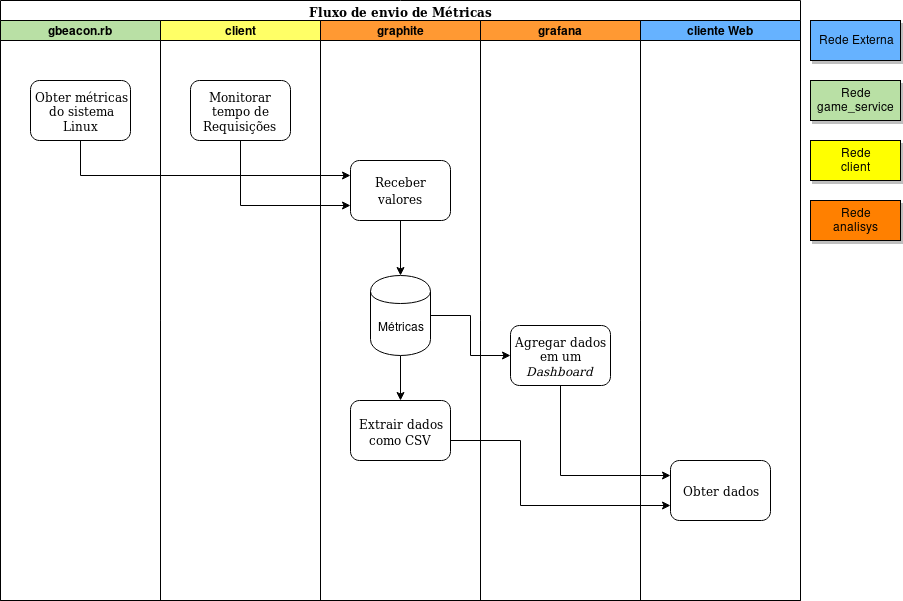
\includegraphics[width=\textwidth]{img/cap5/fluxo_metricas.png}
    \centering
    
    Fonte: O próprio autor
\end{figure}

Como exibido na Figura~\ref{fig:fluxo_data}, existem dois tipos de monitores que populam os dados automaticamente no sistema de monitoramento.
%
São eles o monitor de recursos e  o monitor de tempo de requisição. 

O monitor de recursos é utilizado no \textit{game\_service} enviando métricas do consumo de recursos pela instância.
%
Este monitor foi implementado para este TCC na linguagem Ruby e é distribuído como uma aplicação completa para monitoramento de sistemas baseados em Debian.
%
O mesmo possui a automatização de implantação do servidor Graphite e Grafana utilizando Docker Compose em seu repositório~\footnote{gbeacon.rb: \url{github.com/schweigert/grafana-beacon/} e \url{rubygems.org/gems/gbeacon}}.

Durante os experimentos é executado o monitor de recursos na arquitetura do \textit{game\_service}, a qual envia as métricas obtidas do sistema operacional para o servidor Graphite indicado.
%
Este monitor obtém os recursos programados da máquina hospedeira, na qual hospeda o serviço de jogo utilizando o orquestrador Docker Swarm.
%
Dessa forma temos o monitoramento de recursos em tempo de execução, levando em consideração o custo de gerenciamento da arquitetura.
%
Entretanto, após as capturas de métricas, o consumo de recursos para gestão mostrou-se desprezível para tal experimento.

Por sua vez, o monitor de tempo de resposta é implementado diretamente no cliente, capturando o tempo das requisições do serviço do jogo.
%
Este foi isolado em um pacote na linguagem Golang, na qual pode ser reutilizado em futuros projetos~\footnote{metric package: \url{https://github.com/schweigert/mga/tree/master/libraries/metric}}.

Após a coleta de dados durante os experimentos, os dados são analisados tanto nos gráficos padrões de monitoramento do Grafana, nos pós processados por outras ferramentas como o Gnuplot~\footnote{Gnuplot: \url{http://www.gnuplot.info/}}, os quais são obtidos através da \ac{api} de \textit{render}~\footnote{Graphite render API: \url{https://graphite.readthedocs.io/en/latest/render_api.html}} do Graphite no formato \ac{json} ou \ac{csv}.
%
Dessa forma, também existe a flexibilidade de obter métricas para estudos estatísticos externos a pilha padrão do Graphite/Grafana.



\section{Arquitetura Rudy}
\label{sec:arc_rudy}

A arquitetura Rudy (Subseção~\ref{rudy}) é a primeira arquitetura desenvolvida.
%
Esta teve o seu funcionamento reduzido aos microsserviços básicos da arquitetura para permitir o funcionamento do Gerente de Mundo.
%
Os serviços de Pagamento e Web Estático foram removidos, visto que não condizem ao escopo do atual trabalho.
%
Nesse sentido, os microsserviços implementados são:

\begin{enumerate}
    \item Serviço de Jogo (\textit{rudygh}).
    \item Gerenciador de Consultas (\textit{rudydb}).
    \item Serviço de Autenticação (\textit{rudya}).
    \item Serviço Web Dinâmico (\textit{rudyweb}).
\end{enumerate}
%ccm breve descrição, uma ou dua linhas no máximo.

Além destes microsserviços, a arquitetura utiliza os serviços PostgreSQL e Redis, ambos de código aberto.
%
Tais serviços são utilizados respectivamente como banco de dados permanente e banco de dados em memória cache para autenticação, e foram implantados na sub-rede de banco de dados do jogo.
%
Este método de autenticação foi replicado para as demais arquiteturas.

Em relação aos protocolos utilizados na arquitetura Rudy, a arquitetura utiliza serviços com o protocolos \ac{rpc} e \ac{http}.
%
A relação detalhada é exibida na Tabela~\ref{tab:protocolos_rudy}.



\begin{table}[htb!]
    \centering
    \caption{Protocolos dos microsserviços da arquitetura Rudy.}
    \label{tab:protocolos_rudy}
    \begin{tabular}{|l|l|l|l|}
    \hline
    Microsserviço & Tecnologia utilizada                 & Porta & Protocolo \\ \hline
    rudygh        & Golang 1.11 / RPC Nativo             & 3000  & RPC/TCP       \\ \hline
    rudydb        & Golang 1.11 / Gin \textit{Framework} & 3000  & HTTP      \\ \hline
    rudya         & Golang 1.11 / RPC Nativo             & 3000  & RPC/TCP       \\ \hline
    rudyweb       & Golang 1.11 / Gin \textit{Framework} & 3000  & HTTP      \\ \hline
    \end{tabular}
    
    Fonte: O próprio autor.
\end{table}
%ccm justificar a escolha


Além dos protocolos utilizados, a Tabela~\ref{tab:protocolos_rudy} relaciona as tecnologias utilizadas para implementar o serviço.
%
Tanto os microsserviços da arquitetura Rudy, quanto os demais microsserviços implementados, foram escritos na linguagem Go, evitando a repetição de códigos compartilhados entre eles.
%
Ambos os serviços compartilham dos mesmos modelos de padrão \ac{mvc} para as aplicações \ac{rpc} e \ac{http}.

Para o desenvolvimento dos microsserviços da arquitetura Rudy, foram utilizados os pacotes externos da linguagem:

\begin{itemize}
    \item Gin: \textit{Framework} focado em desenvolvimentos de \ac{api} para web escrito em Golang.
    \item Redis: Pacote de conexão sobre \ac{tcp} ou \ac{udp} em um serviço Redis.
    \item Protofub: Pacote que implementa serialização de dados estruturados de modo compactado. É utilizado para minimizar o gasto de recursos das chamadas \ac{rpc} em Go.
    \item Gorm: Golang \ac{orm} que permite a conexão com o banco de dados Postgres sem utilizar \ac{sql}.
    \item Graphite: Pacote que permite a conexão com o servidor de \textit{logs} Graphite para enviar métricas.
    \item Gorequest: Pacote para estruturar requisições Web utilizado para comunicação interna entre serviços Web utilizando assinatura \ac{jwt}.
    \item Testify: Suíte de testes para manter o funcionamento íntegro durante a implementação da aplicação. Em específico, a aplicação possui 90\% de convergência de código, a qual garante a integridade de futuras alterações.
\end{itemize}

A pilha de desenvolvimento foi escolhida com base na linguagem Golang 1.11, que tem seu foco na legibilidade de código, eficiência computacional (linguagem compilada e tipada) e bibliotecas nativas para sistemas distribuídos.
%
Além de sua eficiência computacional, existe uma comunidade ativa que apoia o desenvolvimento de microsserviços utilizando Golang, contribuindo continuamente com o desenvolvimento de bibliotecas para problemas comuns em sistemas distribuídos sob licença \textit{OpenSource}.
%
Nesse sentido, todas as bibliotecas utilizadas são distribuídas no modelo \textit{Open Source}, pelas licenças \textit{MIT}, \textit{BSD} e \textit{GPLv3}.
%
Estas mesmas bibliotecas são utilizadas nas demais arquiteturas.

 
\section{Dados obtidos da arquitetura Rudy}
\label{sec:dados_rudy}
Para obter os dados da arquitetura Rudy, foram efetuadas três testes diferentes.
%
A diferença entre cada teste é o crescimento de conexões por minuto.
%
Os testes foram automatizados da seguinte maneira:

\begin{itemize}
 \item Escalando um cliente novo por minuto.
 \item Escalando dois clientes novos por minuto.
 \item Escalando cinco clientes novos por minuto.
\end{itemize}

Para cada item citado, a cada minuto, foram escalonados N novos clientes robôs que realizaram as seguintes ações:

\begin{itemize}
 \item Criar uma conta.
 \item Autenticar a conta.
 \item Criar um personagem.
 \item Selecionar personagem.
 \item Movimentar-se pelo jogo, enviar mensagens e receber mensagens. %ccm por quanto tempo ou qtde. movimentos. Alternativa mencionar a seção do automato.
\end{itemize}

Dentro deste cenário, esperava-se estressar a vazão da rede ou \ac{cpu}, visto que são poucos dados para armazenamento em memória do serviço de jogo.
%
Tal qual, esta especulação foi confirmada devido a fila de processamento de requisições da arquitetura Rudy não escalar para múltiplos usuários em uma única região.
%
Vale ressaltar que a latência da rede não foi prejudicada durante o teste, tornando-se constante, como já esperado.


\subsection{Consumo de CPU}

Um dos objetivos da coleta de \ac{cpu} da arquitetura Rudy é analisar possíveis pontos de gargalo no processamento das requisições.
%
Em especial a arquitetura Rudy tem uma abordagem serial das requisições, a qual serve para evitar a concorrência das estruturas de dados internas entre múltiplos jogadores.
%
Entretanto, espera-se um enfileiramento das requisições para operações na mesma região do ambiente do jogo.
%
Neste sentido, tal resultado tende a um ponto limitante de processamento na arquitetura Rudy.

As variáveis relacionadas a este experimento são o número de conexões e o número de requisições na fila.
%
A Figura~\ref{fig:rudy_t4_cpu} exibe a carga da \ac{cpu} e carga do Sistema Operacional no serviço de jogo.


\begin{figure}[htb!]
    \caption{Consumo de \ac{cpu} no servidor utilizando a arquitetura Rudy ($N=1$)}
    \label{fig:rudy_t4_cpu}
    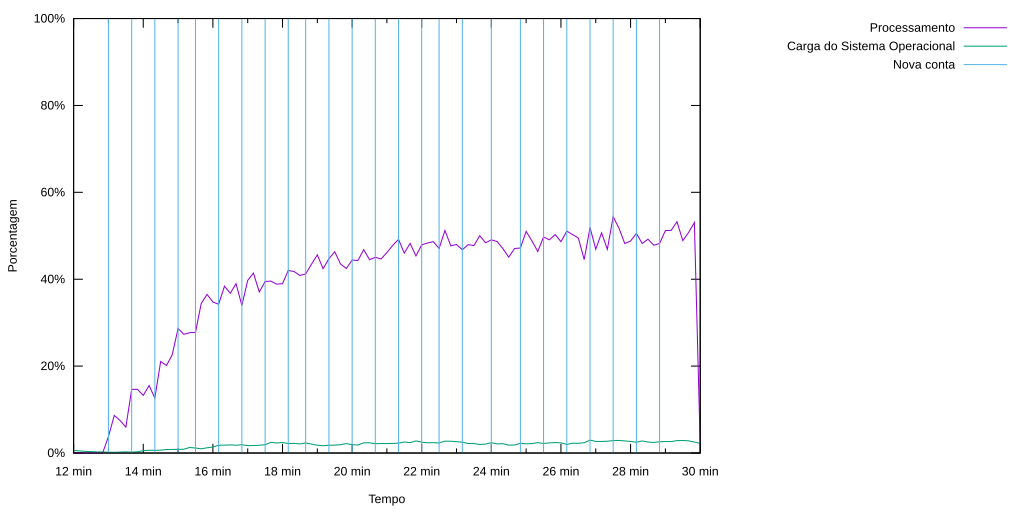
\includegraphics[width=\textwidth]{metricas_rudy_t4/cpu.png}
    \centering
    
    Fonte: O próprio autor
\end{figure}
%ccm explicar que as linhas verticais são novos clientes

Como observado na Figura~\ref{fig:rudy_t4_cpu}, houve um limite do consumo de \ac{cpu} por parte do serviço, que foi ocasionado pela fila de requisições.
%
Em específico, o sistema perdeu desempenho no enfileiramento das requisições nas barreiras de processamento do serviço.
%
A partir de um número determinado de conexões (entre 7 e 10 conexões no experimento da Figura~\ref{fig:rudy_t4_cpu}) na mesma região do ambiente de jogo, a disputa para enfileirar novas requisições é alta o suficiente para o processamento das requisições ser insuficiente sob tal demanda.
%
Um dos pontos que provam tal ocorrência é uma barreira na vazão de rede, que correlaciona com a \ac{cpu} e o aumento do tempo de resposta do serviço.

Conforme os dados obtidos do primeiro experimento, é previsto que o mesmo comportamento ocorra, de forma mais agressiva, para os testes com a escalabilidade de $N=2$ e $N=5$.
%
O comportamento nos Experimentos 2 e 3 pode ser visualizado na Figura~\ref{fig:rudy_t56_cpu}.

\begin{figure}[htb!]
    \caption{Consumo de \ac{cpu} no servidor utilizando a arquitetura Rudy ($N=2$ e $N=5$)}
    \centering
    \begin{subfigure}{1.0\textwidth}
      \centering
      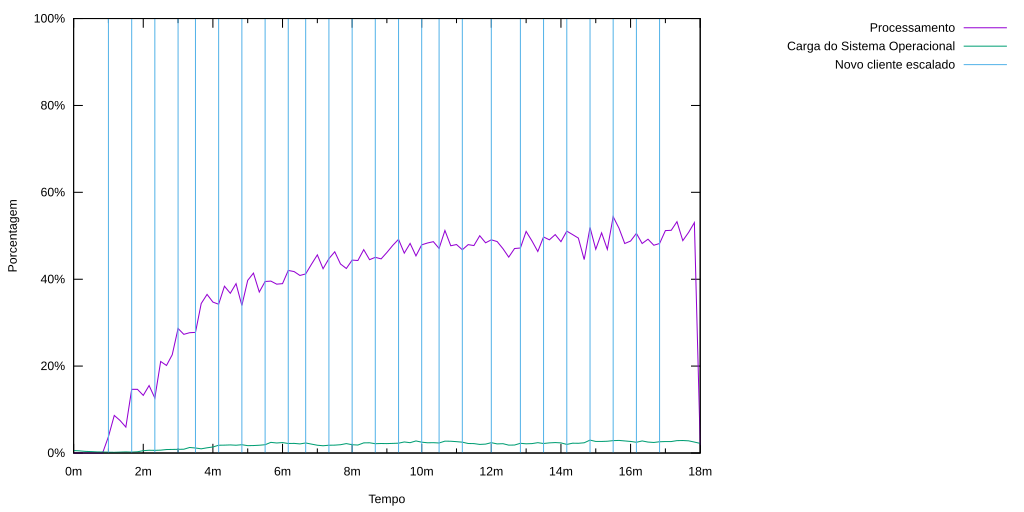
\includegraphics[width=.9\textwidth]{metricas_rudy_t5/cpu.png}
      \caption{Consumo de \ac{cpu} no servidor utilizando a arquitetura Rudy ($N=2$)}
      \label{fig:rudy_t5_cpu}
    \end{subfigure}


    \begin{subfigure}{1.0\textwidth}
      \centering
      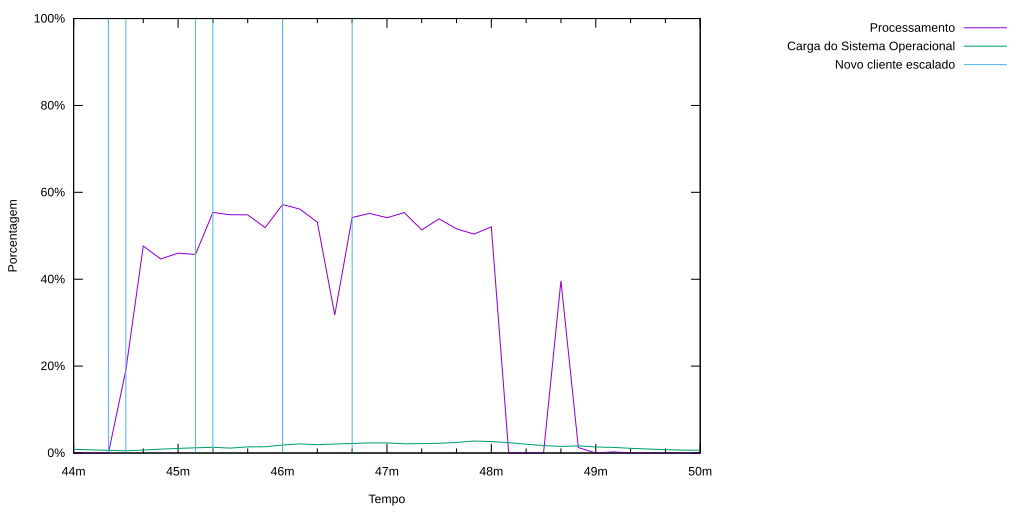
\includegraphics[width=.9\textwidth]{metricas_rudy_t6/cpu.png}
      \caption{Consumo de \ac{cpu} no servidor utilizando a arquitetura Rudy ($N=5$)}
      \label{fig:rudy_t6_cpu}
    \end{subfigure}
    \label{fig:rudy_t56_cpu}

    Fonte: O próprio autor.
\end{figure}
% fazer uma figura para cada um.
A Figura~\ref{fig:rudy_t56_cpu} exibe o mesmo comportamento de enfileiramento de requisições da arquitetura ~\ref{fig:rudy_t4_cpu}.
%
Dessa forma, torna-se notório a interferência das barreiras para serializar as requisições ao serviço.
%


\subsection{Consumo de Memória}

O principal objetivo da coleta de memória da arquitetura Rudy é analisar possíveis vulnerabilidades a qual podem ser sanadas com a escalabilidade do sistema.
%
Em geral, jogos \ac{mmorpg} permitem a divisão de suas regiões em \textit{chunks}, a qual são distribuídos entre os serviços.
%
Esta divisão de carga também é aplicada na arquitetura Rudy.
%
Dessa forma, espera-se que a memória seja impactada pelo número de conexões simultâneas em um único pedaço do mundo, consumindo memória para processamento do protocolo \ac{rpc} e armazenamento dos dados do cliente e do mundo, a qual consomem recursos conforme a regra de negócio.

Outro ponto de consumo da memória é referente ao consumo da pilha de execução das chamadas web. Em geral, esta aplicação só consumirá memória especificamente durante a requisição, no qual armazenará o estado no banco de dados, não precisando executar outras operações para manutenção da memória local.
%
Nesse sentido, este teste tende a ter um baixo consumo de memória, visto que as regras de negócio são simples e a memória tende a ser linearmente consumida conforme o número de conexões simultâneas.

O teste executado na arquitetura obteve os dados que condizem com a expectativa dos testes, obtendo um baixo consumo de recursos por parte das aplicações da arquitetura Rudy.
%
A Figura~\ref{fig:rudy_t4_memory} compara a memória total com a memória utilizada pela arquitetura.

\begin{figure}[htb!]
    \caption{Registro de memória no servidor utilizando a arquitetura Rudy}
    \label{fig:rudy_t4_memory}
    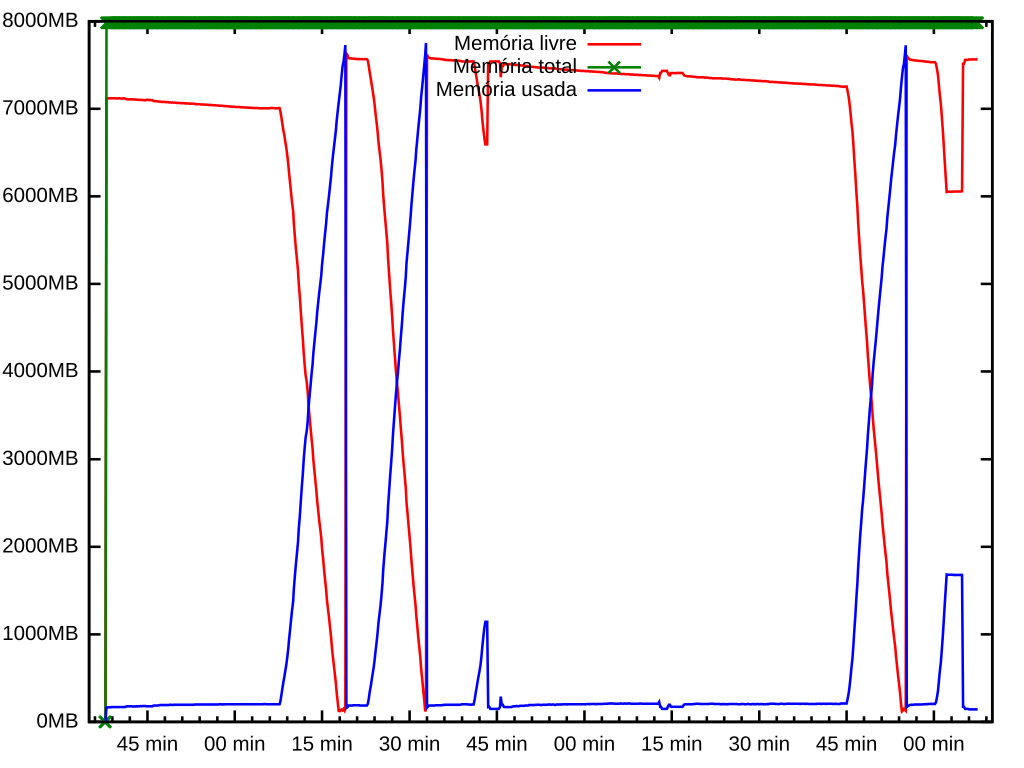
\includegraphics[width=\textwidth]{metricas_rudy_t4/memory.png}
    \centering
    
    Fonte: O próprio autor
\end{figure}

A comparação exibida na Figura~\ref{fig:rudy_t4_memory} mostra somente a escala entre a memória total do serviço com relação a memória consumida.
%
Porém, esta visualização fica comprometida, visto que não fica perceptível a baixa variação da memória consumida com relação ao número de conexões no serviço.
%
A Figura~\ref{fig:rudy_t4_memory_used} trata a escala e aplica somente os dados da memória utilizada pela arquitetura.

\begin{figure}[htb!]
    \caption{Memória consumida no servidor utilizando a arquitetura Rudy ($N=1$)}
    \label{fig:rudy_t4_memory_used}
    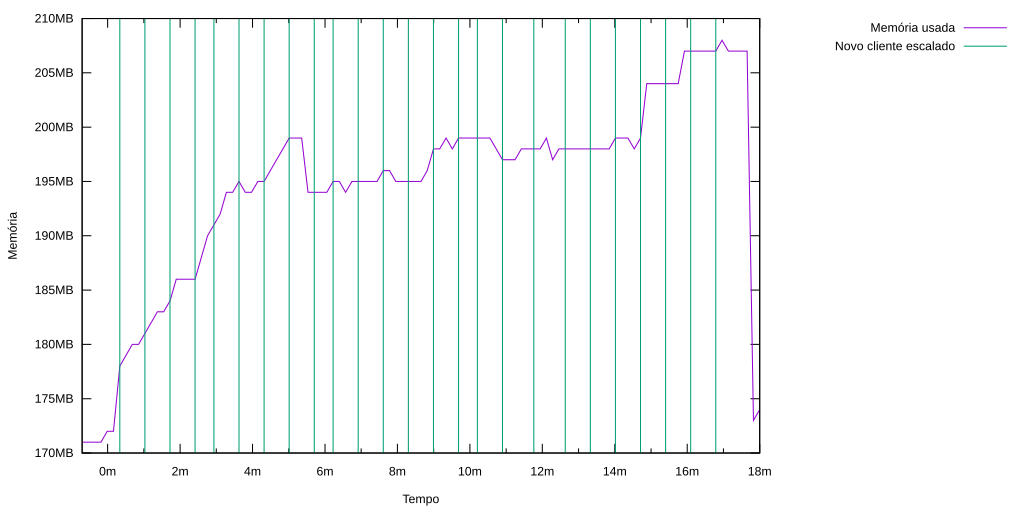
\includegraphics[width=\textwidth]{metricas_rudy_t4/memory_used.png}
    \centering
    
    Fonte: O próprio autor
\end{figure}

Após o tratamento, torna-se notório o crescimento da memória conforme o número de conexões, utilizando uma alícota de valor pequeno, se comparado ao recurso disponível.
%
Nesse sentido, não foi possível estressar a memória do serviço como um recurso crítico para os testes, porém isto não invalida estes dados para futura comparação com as demais arquiteturas.

\begin{figure}[htb!]
    \caption{Memória consumida no servidor utilizando a arquitetura Rudy ($N=2$ e $N=5$)}
    \centering
    \begin{subfigure}{1.0\textwidth}
      \centering
      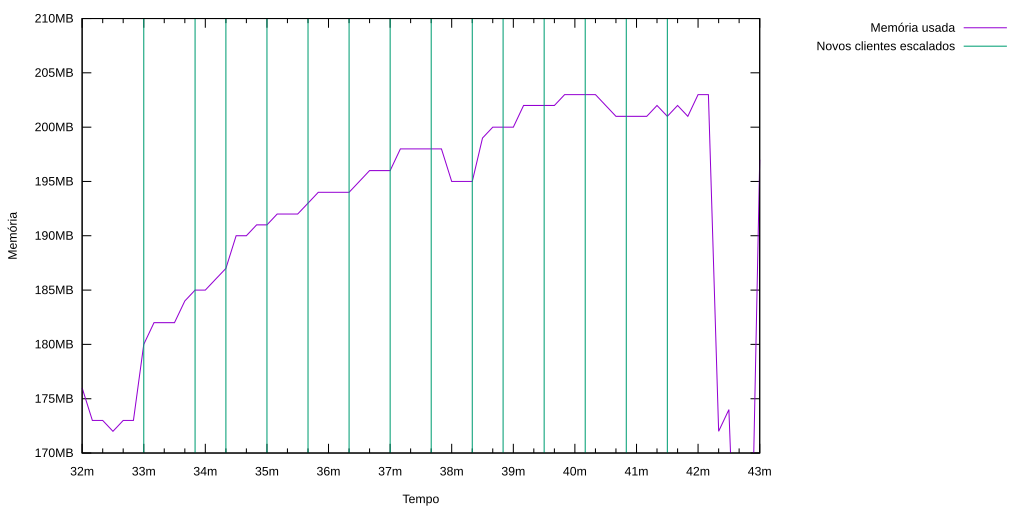
\includegraphics[width=.9\textwidth]{metricas_rudy_t5/memory_used.png}
      \caption{Memória consumida no servidor utilizando a arquitetura Rudy ($N=2$)}
      \label{fig:rudy_t5_memory_used}
    \end{subfigure}


    \begin{subfigure}{1.0\textwidth}
      \centering
      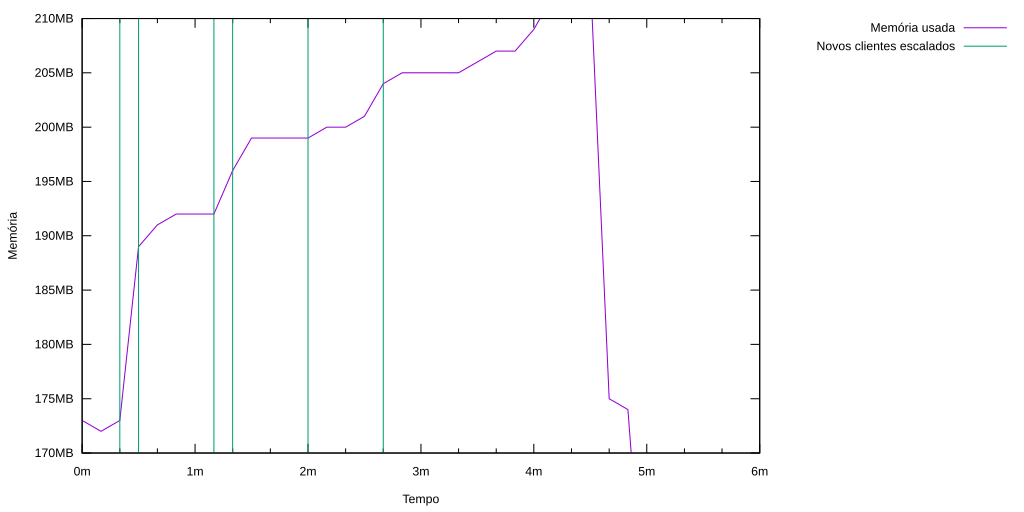
\includegraphics[width=.9\textwidth]{metricas_rudy_t6/memory_used.png}
      \caption{Memória consumida no servidor utilizando a arquitetura Rudy ($N=5$)}
      \label{fig:rudy_t6_memory_used}
    \end{subfigure}
    \label{fig:rudy_t56_memory_used}

    Fonte: O próprio autor.
\end{figure}

\subsection{Consumo de Banda}

O principal objetivo do monitoramento do consumo da banda pelo serviço Rudy é verificar se a rede está enfileirando as requisições nos serviços \ac{rpc} na arquitetura.
%
Esta validação é feita caso a rede tenha um limite notório na entrada e saída da rede e o aumento do tempo de requisição, sem comprometer a \ac{cpu} do serviço.

Caso as requisições sejam enfileiradas internamente pelo microsserviço \ac{rpc} (Gerente de Jogo), como o modelo de processamento de requisições da arquitetura Rudy propõe, espera-se que o tempo de resposta que aumente.
%
O aumento do tempo de resposta é um reflexo da concorrência para escrever a requisição \ac{rpc} na fila de processamento do serviço, a qual dependerá do escalonador de \textit{threads} escolher qual processo escreverá a sua requisição na fila.

Com os dados da banda da arquitetura Rudy obtidos do teste, pode-se observar que o crescimento do consumo da rede não é linear.
%
Os dados podem ser visualizados na Figura~\ref{fig:rudy_t4_io}.

\begin{figure}[htb!]
    \caption{Consumo de Banda no servidor utilizando a arquitetura Rudy ($N=1$)}
    \label{fig:rudy_t4_io}
    \includegraphics[width=\textwidth]{metricas_rudy_t4/io.png}
    \centering
    
    Fonte: O próprio autor
\end{figure}

\begin{figure}[htb!]
    \caption{Consumo de Banda no servidor utilizando a arquitetura Rudy ($N=2$ e $N=5$)}
    \centering
    \begin{subfigure}{1.0\textwidth}
      \centering
      \includegraphics[width=.9\textwidth]{metricas_rudy_t5/io.png}
      \caption{Consumo de Banda no servidor utilizando a arquitetura Rudy ($N=2$)}
      \label{fig:rudy_t5_io}
    \end{subfigure}


    \begin{subfigure}{1.0\textwidth}
      \centering
      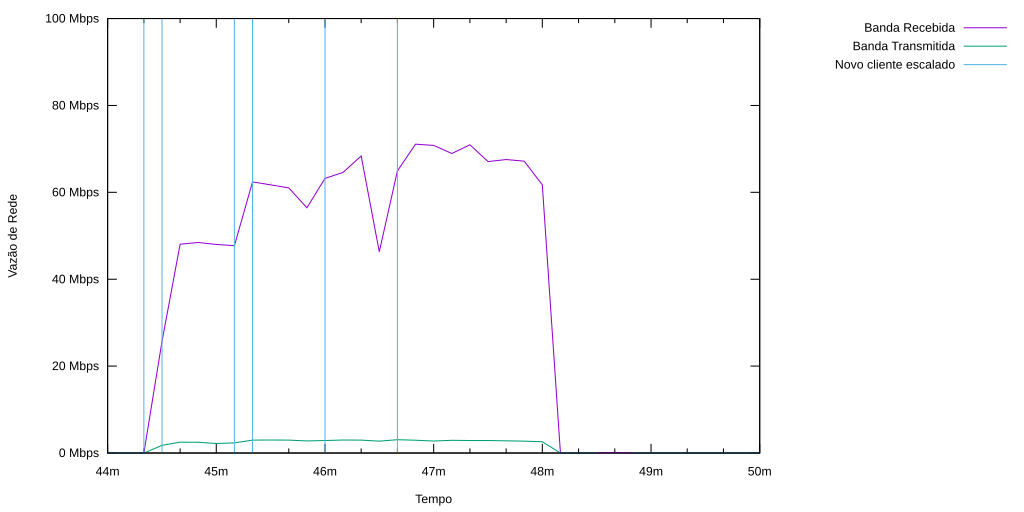
\includegraphics[width=.9\textwidth]{metricas_rudy_t6/io.png}
      \caption{Consumo de Banda no servidor utilizando a arquitetura Rudy ($N=5$)}
      \label{fig:rudy_t6_io}
    \end{subfigure}
    \label{fig:rudy_t56_io}

    Fonte: O próprio autor.
\end{figure}

Como observado na Figura~\ref{fig:rudy_t4_io}, existe um limite de crescimento da banda.
%
Com as configurações do ambiente, este valor tende a 60Mbps.
%
Vale ressaltar que este gargalo não é proveniente da rede (a qual ficou limitada em 100Mbps), visto que a métrica de latência ficou constante durante os testes.
%
Dessa forma, esta tendência pode ser pela concorrência a fila de processamento, a qual espera-se confirmar com o tempo de resposta do cliente.


\subsection{Tempo de Resposta do cliente}

Para a arquitetura Rudy, o tempo de resposta do cliente irá confirmar se o enfileiramento das requisições \ac{rpc} ocorreram como previsto.
%
Nesse sentido, espera-se que o tempo de requisição aumente de forma superlinear conforme o número de clientes escalados aumente.


Além disso, será possível visualizar o impacto de operações realizadas no banco com o tempo de resposta do serviço, visto que ao efetuar uma operação no banco a mensagem será transmitida pelos microsserviços web dinâmico e pelo gestor do banco de dados, além do banco de dados por fim.
%
Este impácto chamadas sobre o protocolo \ac{http} com múltiplas camadas deve ser notório conforme a demanda de usuários, atrapalhando o gestor de rede com o consumo de \ac{cpu} e rede para atende-los.

Para comparação entre as requisições \ac{rpc} e web, a Figura~\ref{fig:rudy_t4_reqs} exibe ambas em uma única Figura.
%
Espera-se mostrar o crescimento superlinear das requisições \ac{rpc}, a qual chegam a ultrapassar o tempo de resposta das requisições \ac{http} com múltiplas camadas.

\begin{figure}[htb!]
    \caption{Tempo de Resposta do cliente servidor utilizando a arquitetura Rudy ($N=1$)}
    \label{fig:rudy_t4_reqs}
    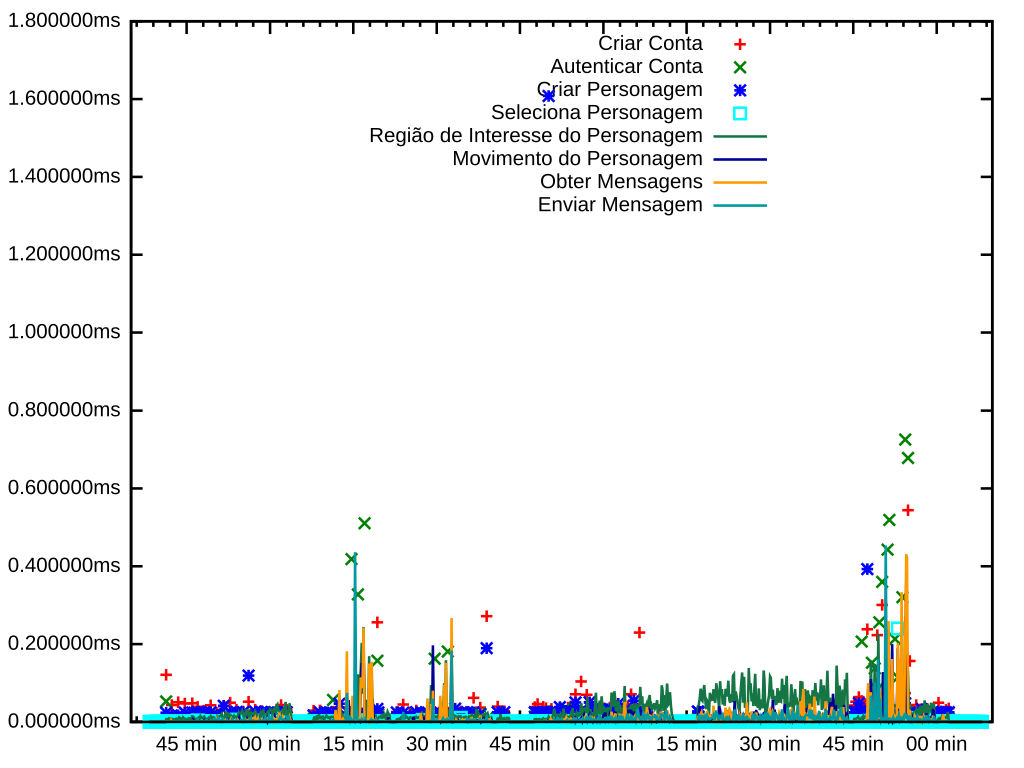
\includegraphics[width=\textwidth]{metricas_rudy_t4/rudyc.png}
    \centering
    
    Fonte: O próprio autor
\end{figure}

\begin{figure}[htb!]
    \caption{Tempo de Resposta do cliente servidor utilizando a arquitetura Rudy ($N=2$ e $N=5$)}
    \centering
    \begin{subfigure}{1.0\textwidth}
      \centering
      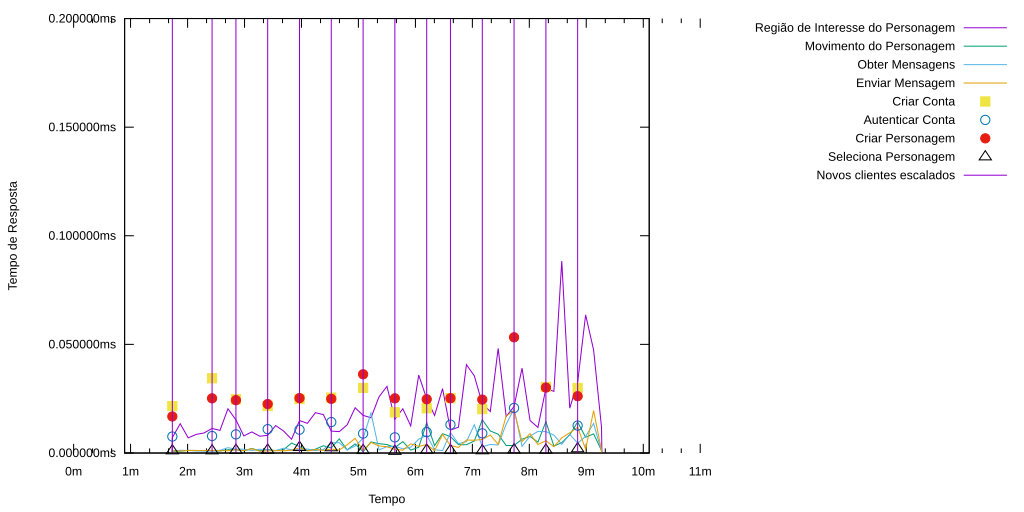
\includegraphics[width=.9\textwidth]{metricas_rudy_t5/rudyc.png}
      \caption{Tempo de Resposta do cliente servidor utilizando a arquitetura Rudy ($N=2$)}
      \label{fig:rudy_t5_reqs}
    \end{subfigure}


    \begin{subfigure}{1.0\textwidth}
      \centering
      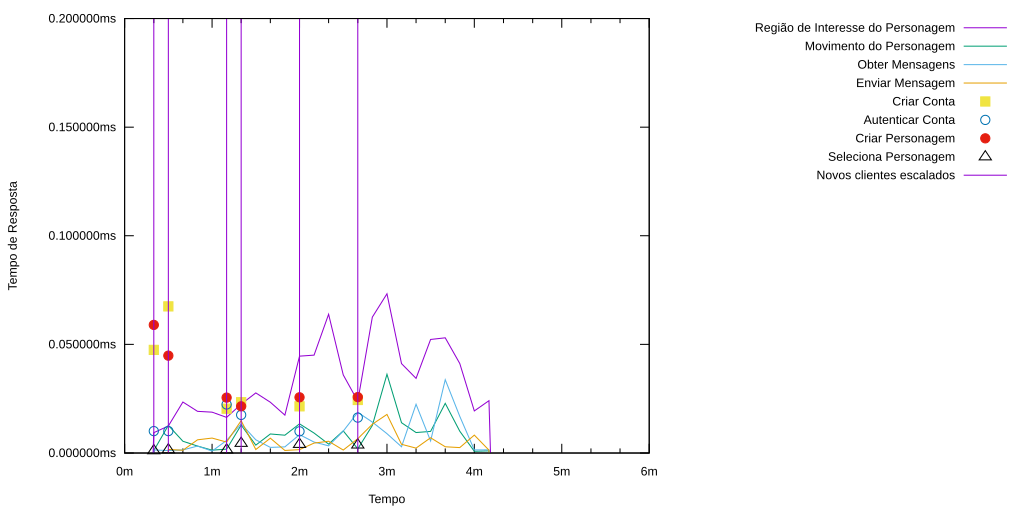
\includegraphics[width=.9\textwidth]{metricas_rudy_t6/rudyc.png}
      \caption{Tempo de Resposta do cliente servidor utilizando a arquitetura Rudy ($N=5$)}
      \label{fig:rudy_t6_reqs}
    \end{subfigure}
    \label{fig:rudy_t56_reqs}

    Fonte: O próprio autor.
\end{figure}

A Figura~\ref{fig:rudy_t4_reqs} mostra, dentro de um intervalo de tempo, o tempo de resposta categorizado conforme a ação realizada pelo cliente no serviço.
%
Para facilitar a visualização, este gráfico foi dividido em duas categorias, segregando as requisições sobre \ac{http} e sobre \ac{rpc}.
%
A Figura~\ref{fig:rudy_t4_reqs_https} exibe o tempo de resposta das requisições web em relação ao tempo.
%
Mostra-se na figura a dispersão que ocorre nos tempos de requisições sobre o protocolo \ac{http} conforme o recurso do serviço é consumido por novos clientes.
 

\begin{figure}[htb!]
    \caption{Tempo de Resposta de requisições \textit{Web} do cliente servidor utilizando a arquitetura Rudy ($N=1$)}
    \label{fig:rudy_t4_reqs_https}
    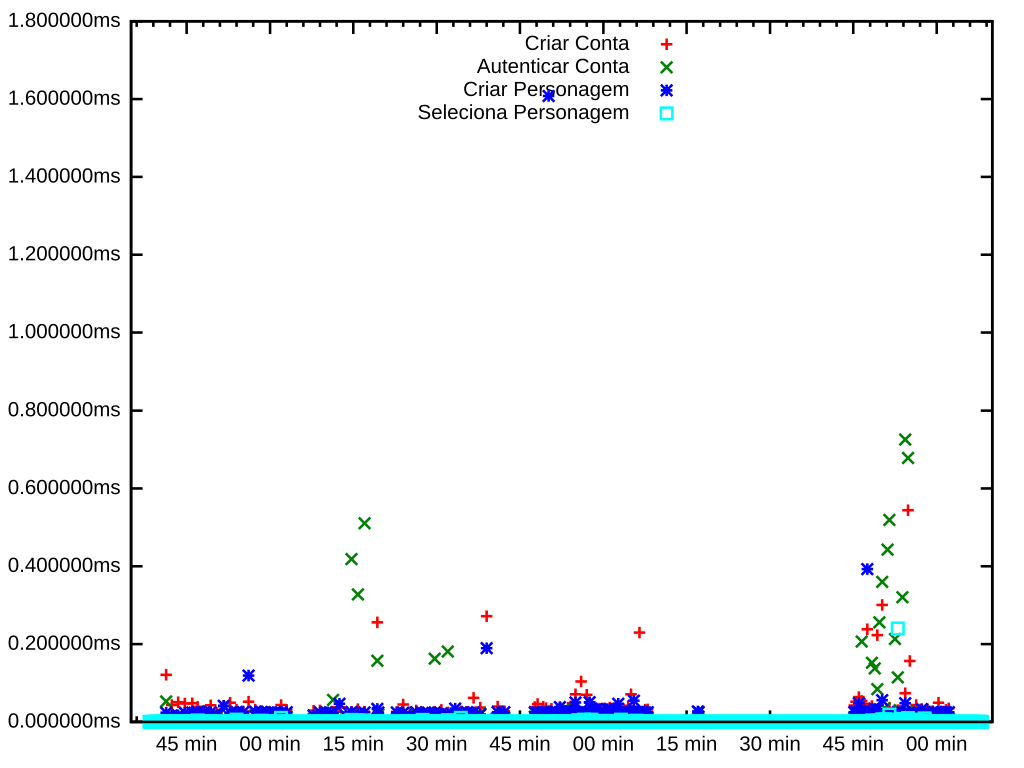
\includegraphics[width=\textwidth]{metricas_rudy_t4/rudyc_http.png}
    \centering
    
    Fonte: O próprio autor
\end{figure}

\begin{figure}[htb!]
    \caption{Tempo de Resposta de requisições \textit{Web} do cliente servidor utilizando a arquitetura Rudy ($N=2$ e $N=5$)}
    \centering
    \begin{subfigure}{1.0\textwidth}
      \centering
      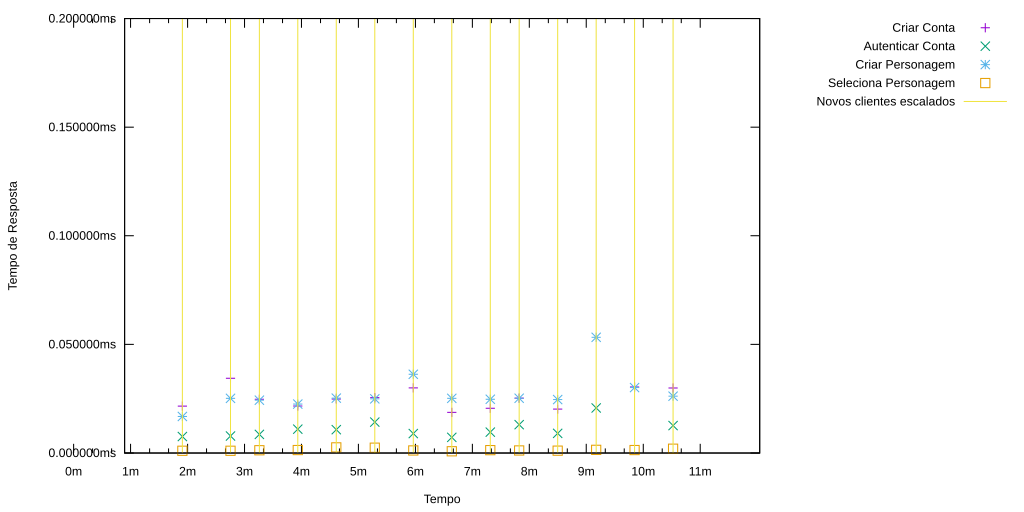
\includegraphics[width=.9\textwidth]{metricas_rudy_t5/rudyc_http.png}
      \caption{Tempo de Resposta de requisições \textit{Web} do cliente servidor utilizando a arquitetura Rudy ($N=2$)}
      \label{fig:rudy_t5_reqs_https}
    \end{subfigure}


    \begin{subfigure}{1.0\textwidth}
      \centering
      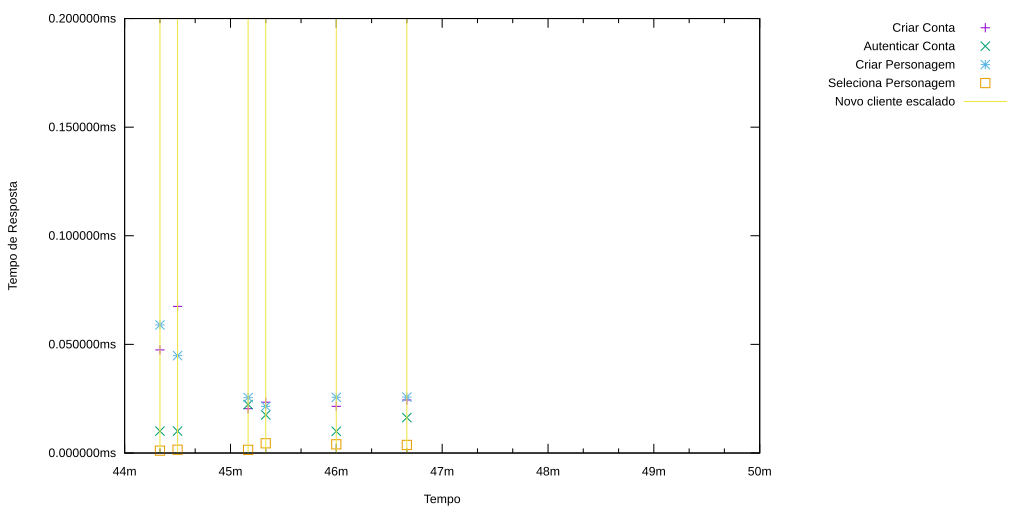
\includegraphics[width=.9\textwidth]{metricas_rudy_t6/rudyc_http.png}
      \caption{Tempo de Resposta de requisições \textit{Web} do cliente servidor utilizando a arquitetura Rudy ($N=5$)}
      \label{fig:rudy_t6_reqs_https}
    \end{subfigure}
    \label{fig:rudy_t56_reqs_https}

    Fonte: O próprio autor.
\end{figure}

A Figura~\ref{fig:rudy_t4_reqs_https} exibe uma dispersão conforme o número de conexões do serviço aumenta.
%
Entretanto, espera-se que este tempo de requisição sobre o protocolo \ac{http} aumente somente como um reflexo do consumo de \ac{cpu} e banda pelos clientes.
%
Por este motivo, é notório a necessidade de exibir a parte o tempo de requisição das chamadas \ac{rpc}.
%
Os dados do protocolo \ac{rpc} podem ser visualizados na Figura~\ref{fig:rudy_t4_reqs_rpc}.

\begin{figure}[htb!]
    \caption{Tempo de Resposta de requisições \ac{rpc} do cliente servidor utilizando a arquitetura Rudy}
    \label{fig:rudy_t4_reqs_rpc}
    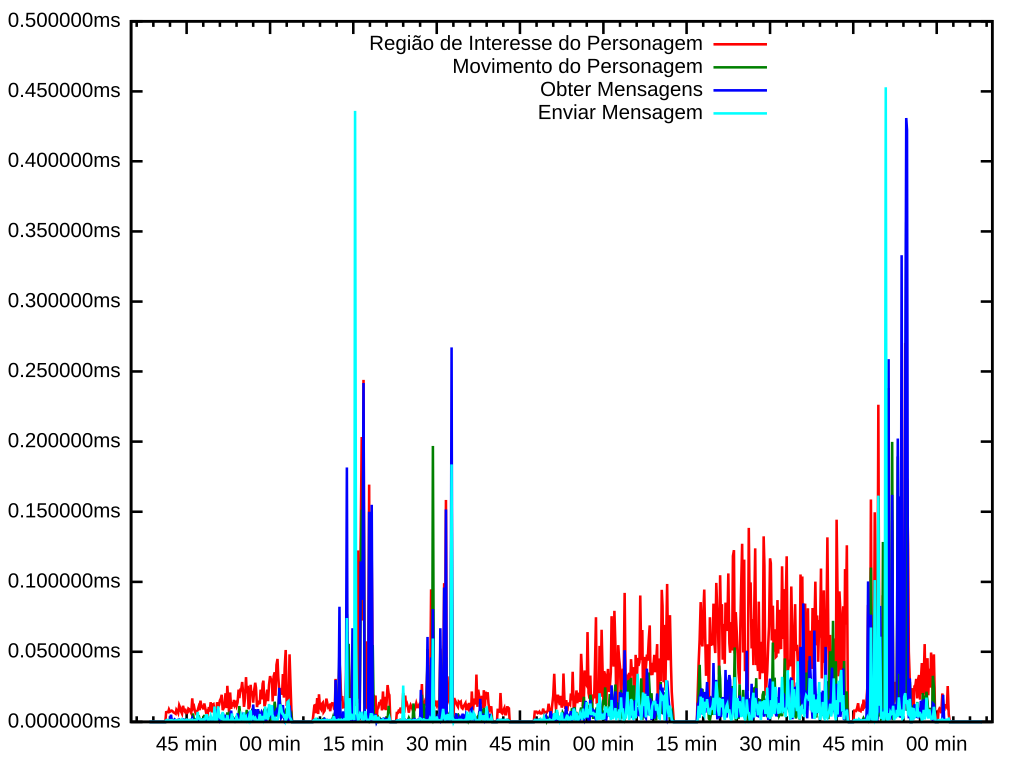
\includegraphics[width=\textwidth]{metricas_rudy_t4/rudyc_rpc.png}
    \centering
    
    Fonte: O próprio autor
\end{figure}

\begin{figure}[htb!]
    \caption{Tempo de Resposta de requisições \textit{rpc} do cliente servidor utilizando a arquitetura Rudy ($N=2$ e $N=5$)}
    \centering
    \begin{subfigure}{1.0\textwidth}
      \centering
      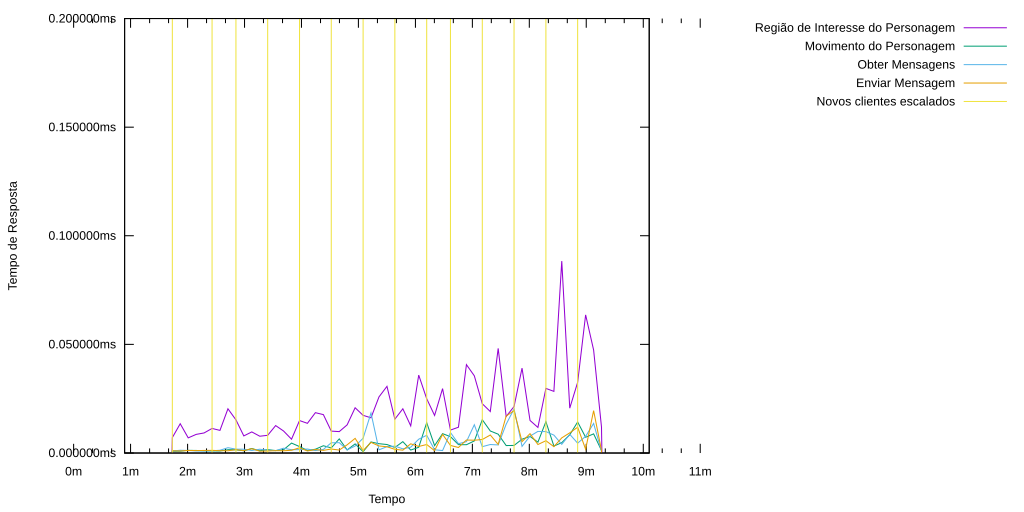
\includegraphics[width=.9\textwidth]{metricas_rudy_t5/rudyc_rpc.png}
      \caption{Tempo de Resposta de requisições \textit{rpc} do cliente servidor utilizando a arquitetura Rudy ($N=2$)}
      \label{fig:rudy_t5_reqs_rpc}
    \end{subfigure}


    \begin{subfigure}{1.0\textwidth}
      \centering
      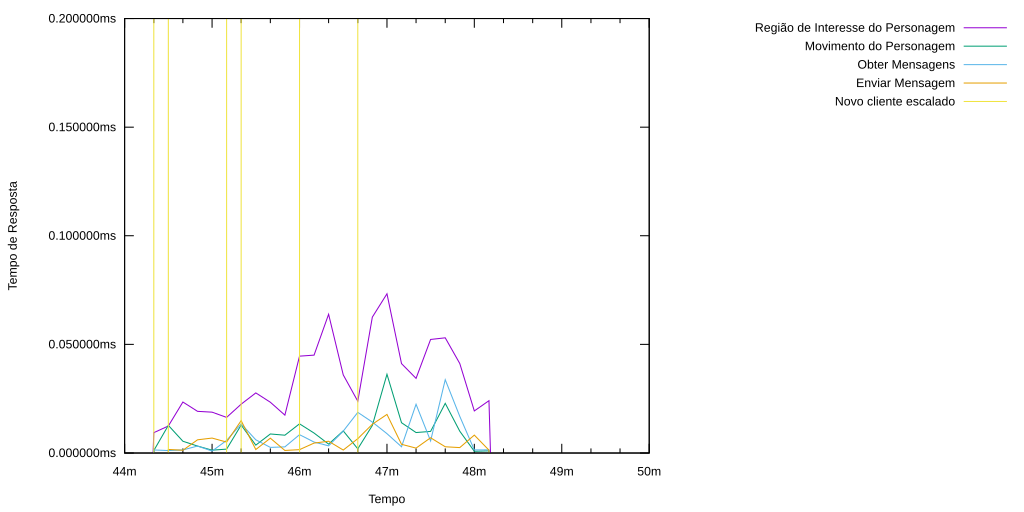
\includegraphics[width=.9\textwidth]{metricas_rudy_t6/rudyc_rpc.png}
      \caption{Tempo de Resposta de requisições \textit{rpc} do cliente servidor utilizando a arquitetura Rudy ($N=5$)}
      \label{fig:rudy_t6_reqs_rpc}
    \end{subfigure}
    \label{fig:rudy_t56_reqs_rpc}

    Fonte: O próprio autor.
\end{figure}

A Figura~\ref{fig:rudy_t4_reqs_rpc} exibe o desparelhamento provocado pelo sistema de filas implementado nesta arquitetura nos serviços \ac{rpc}.
%
Percebe-se também que esta disparidade aumenta diretamente com as requisições \ac{http} ao escalar um novo cliente.
%
Estas informações indicam que de fato ocorre o enfileiramento das requisições, além disso a carga das requisições \ac{http} agravam o enfileiramento, aumentando significantemente o tempo de resposta durante os próximos segundos após a chamada \ac{http}.

A partir dos dados obtidos das requisições \ac{http}, exibidos na Figura~\ref{fig:rudy_t4_reqs_https}, percebe-se que os valores exercem baixa influência conforme a carga de usuários utilizando o serviço.
%
Nesse sentido, é possível agrupar todos os dados a fim de obter a sua média, mediana, valor máximo e mínimo das requisições sobre o protocolo \ac{http}.
%
Estes dados estão dispostos na Tabela~\ref{tab:medias_http_rudy}.

\begin{table}[htb!]
    \centering
    \caption{Média, mediana, máximo e mínimo obtidos pelas requisições HTTP.}
    \label{tab:medias_http_rudy}
    \begin{adjustbox}{width=1\textwidth}
    \begin{tabular}{|l|l|l|l|l|}
    \hline
    Requisição HTTP       & Máximo      & Mínimo        & Média            & Mediana          \\ \hline
    Criar conta           & 0,221395227 s & 0,020872847 s & 0,039408472375 s & 0,0292280260 s \\ \hline
    Autenticar Conta      & 0,207815276 s & 0,007954407 s & 0,019106303125 s & 0,0106579220 s \\ \hline
    Criar Personagem      & 0,090555727 s & 0,019188871 s & 0,027868142025 s & 0,0250552605 s \\ \hline
    Selecionar Personagem & 0,010201612 s & 0,000752974 s & 0,002188604100 s & 0,0021886041 s \\ \hline
    \end{tabular}
    \end{adjustbox}

    Fonte: O próprio autor.
\end{table}

A Tabela~\ref{tab:medias_http_rudy} comprova a estabilidade das requisições \ac{http}, na qual a média, mediana e o valor mínimo estão próximos para todos os tipos de requisição.
%
Nota-se pela Requisição \ac{http} Selecionar Personagem, na qual realiza a busca dos dados no banco em parapelo a requisição, a maior estabilidade e eficiência dentre as demais citadas.
%
Nesse sentido, torna-se visível que a instabilidade, por mais que baixa, esteja relacionada com a busca ou inserção de dados nos bancos da arquitetura.

As requisições \ac{rpc} também podem apresentar caracteristicas similares.
%
Entretanto, as requisições \ac{rpc} concorrem com as requisições \ac{http} entre os recursos do serviço.
%
Nesse sentido, torna-se interessante obter a média, mediana, máximo e mínimo dos tempos de requisição levando em consideração o número de clientes escalados.
%
A Tabela~\ref{tab:medias_rpc_rudy} exibe a média, mediana, máximo e mínimo, segregando conforme o número de conexões do serviço.

\section{Arquitetura Salz}
\label{sec:arc_salz}

\subsection{Consumo de CPU}

\begin{figure}[htb!]
  \caption{Consumo de \ac{cpu} no servidor utilizando a arquitetura Salz ($N=1$)}
  \label{fig:salz_t2_cpu}
  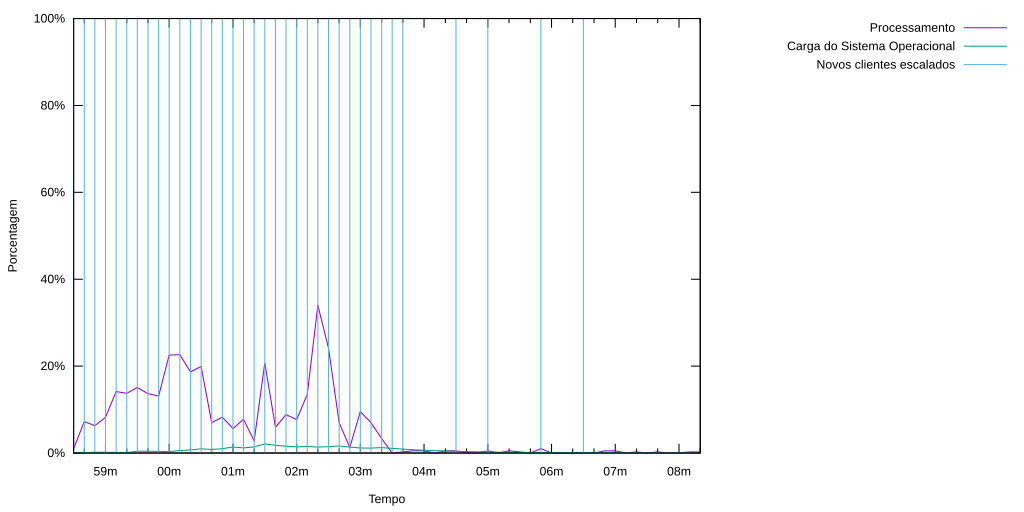
\includegraphics[width=\textwidth]{metricas_salz_t2/cpu.png}
  \centering
  
  Fonte: O próprio autor
\end{figure}

\begin{figure}[htb!]
  \caption{Consumo de \ac{cpu} no servidor utilizando a arquitetura Salz ($N=2$ e $N=5$)}
  \centering
  \begin{subfigure}{1.0\textwidth}
    \centering
    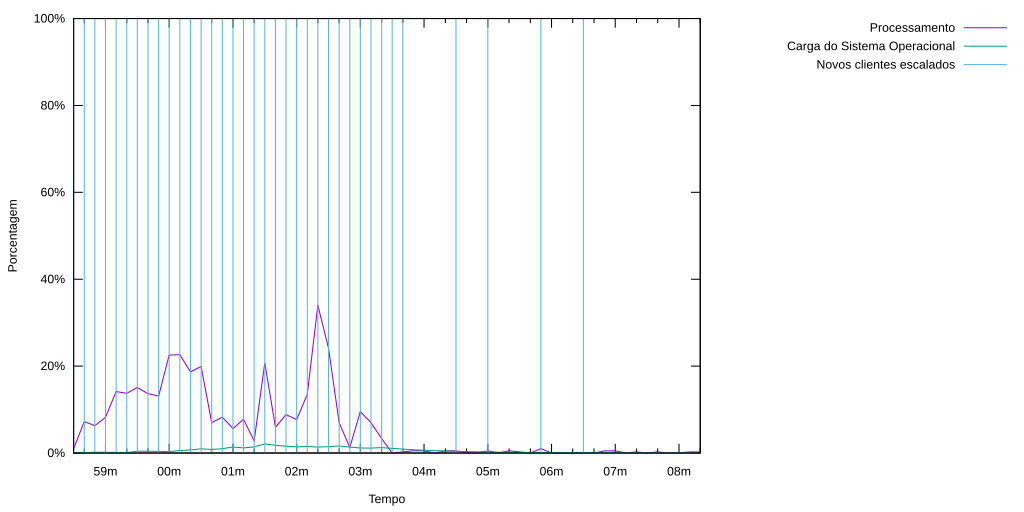
\includegraphics[width=.9\textwidth]{metricas_salz_t2/cpu.png}
    \caption{Consumo de \ac{cpu} no servidor utilizando a arquitetura Salz ($N=2$)}
    \label{fig:rudy_t5_cpu}
  \end{subfigure}


  \begin{subfigure}{1.0\textwidth}
    \centering
    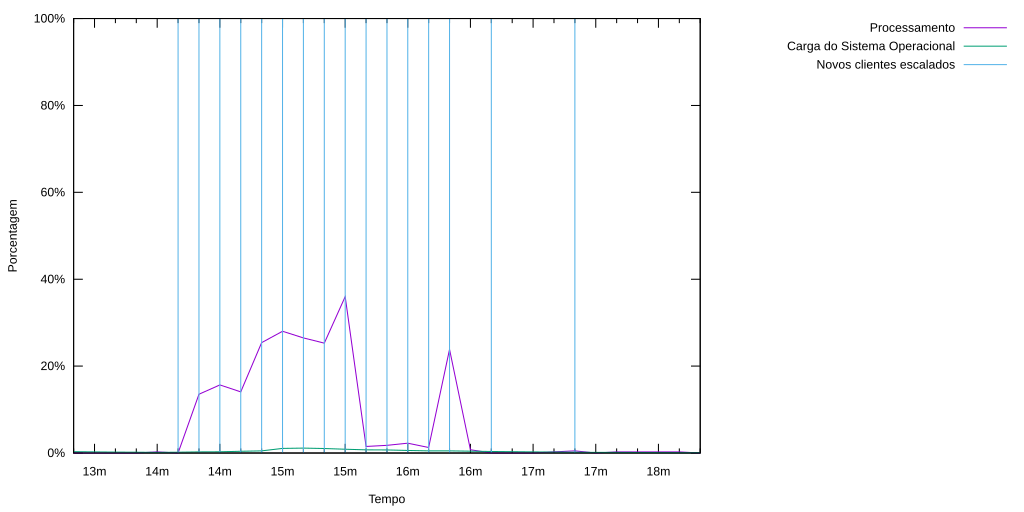
\includegraphics[width=.9\textwidth]{metricas_salz_t3/cpu.png}
    \caption{Consumo de \ac{cpu} no servidor utilizando a arquitetura Salz ($N=5$)}
    \label{fig:rudy_t6_cpu}
  \end{subfigure}
  \label{fig:rudy_t56_cpu}

  Fonte: O próprio autor.
\end{figure}

\subsection{Consumo de Memória}

\begin{figure}[htb!]
  \caption{Memória consumida no servidor utilizando a arquitetura Salz ($N=1$)}
  \label{fig:rudy_t4_memory_used}
  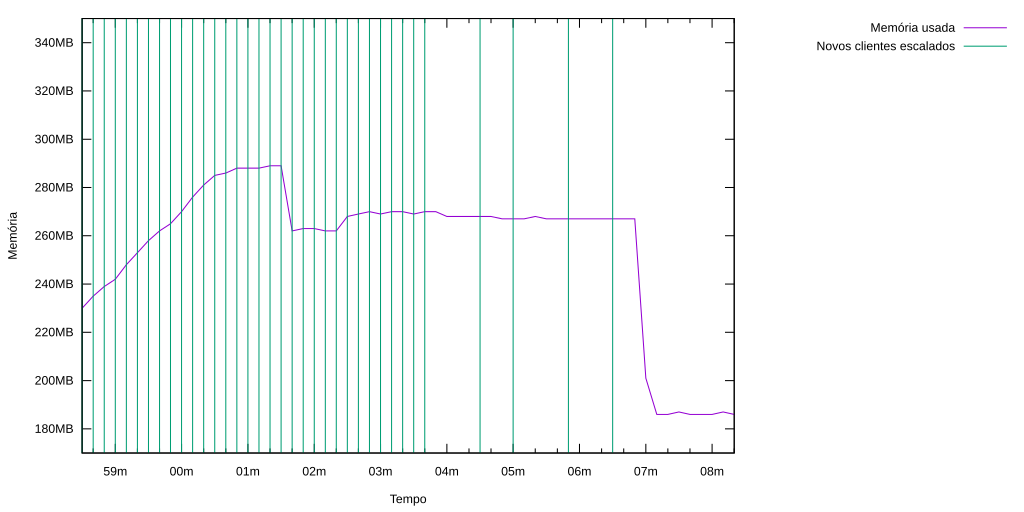
\includegraphics[width=\textwidth]{metricas_salz_t2/memory_used.png}
  \centering
  
  Fonte: O próprio autor
\end{figure}


\begin{figure}[htb!]
  \caption{Memória consumida no servidor utilizando a arquitetura Salz ($N=2$ e $N=5$)}
  \centering
  \begin{subfigure}{1.0\textwidth}
    \centering
    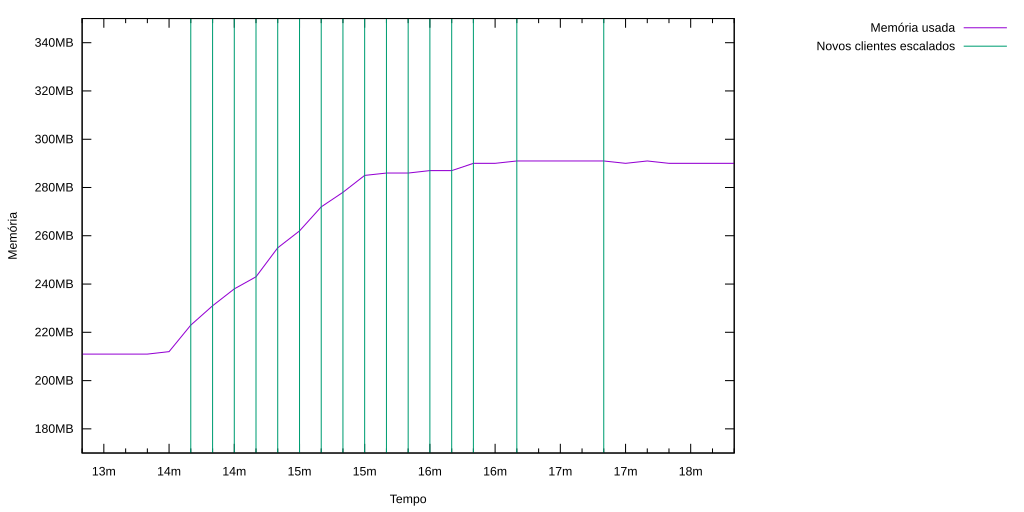
\includegraphics[width=.9\textwidth]{metricas_salz_t3/memory_used.png}
    \caption{Memória consumida no servidor utilizando a arquitetura Salz ($N=2$)}
    \label{fig:rudy_t5_memory_used}
  \end{subfigure}


  \begin{subfigure}{1.0\textwidth}
    \centering
    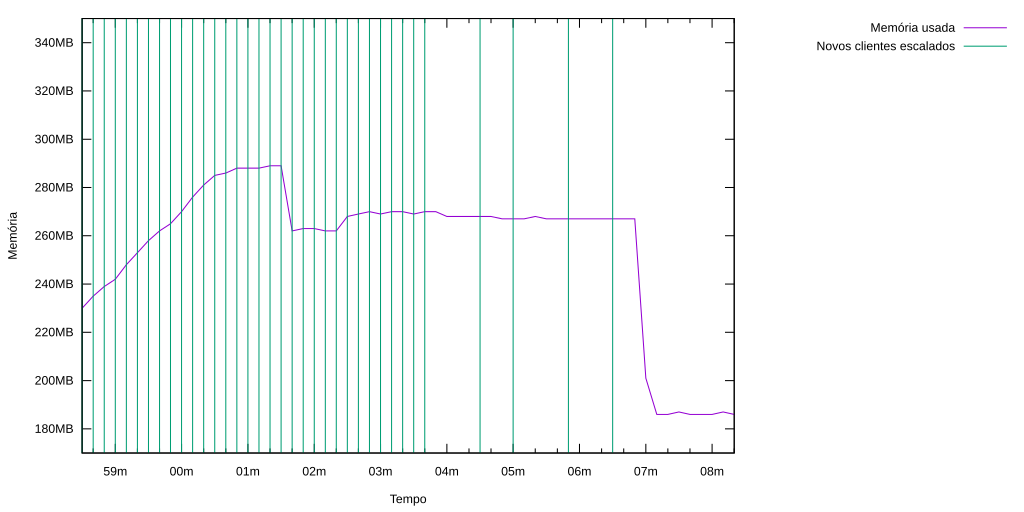
\includegraphics[width=.9\textwidth]{metricas_salz_t2/memory_used.png}
    \caption{Memória consumida no servidor utilizando a arquitetura Salz ($N=5$)}
    \label{fig:rudy_t6_memory_used}
  \end{subfigure}
  \label{fig:rudy_t56_memory_used}

  Fonte: O próprio autor.
\end{figure}


\subsection{Consumo de Banda}

\begin{figure}[htb!]
  \caption{Consumo de Banda no servidor utilizando a arquitetura Salz ($N=1$)}
  \label{fig:rudy_t4_io}
  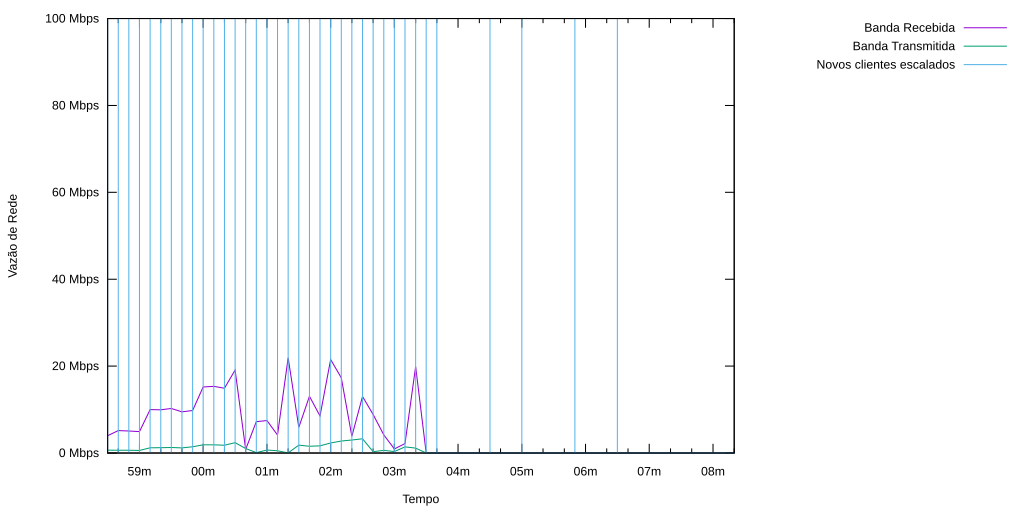
\includegraphics[width=\textwidth]{metricas_salz_t2/io.png}
  \centering
  
  Fonte: O próprio autor
\end{figure}

\begin{figure}[htb!]
  \caption{Consumo de Banda no servidor utilizando a arquitetura Salz ($N=2$ e $N=5$)}
  \centering
  \begin{subfigure}{1.0\textwidth}
    \centering
    \includegraphics[width=.9\textwidth]{metricas_salz_t3/io.png}
    \caption{Consumo de Banda no servidor utilizando a arquitetura Salz ($N=2$)}
    \label{fig:rudy_t5_io}
  \end{subfigure}


  \begin{subfigure}{1.0\textwidth}
    \centering
    \includegraphics[width=.9\textwidth]{metricas_salz_t2/io.png}
    \caption{Consumo de Banda no servidor utilizando a arquitetura Salz ($N=5$)}
    \label{fig:rudy_t6_io}
  \end{subfigure}
  \label{fig:rudy_t56_io}

  Fonte: O próprio autor.
\end{figure}


\subsection{Tempo de Resposta do cliente}

\chapter{Experimentos \& Análises}
\label{cap6}



A partir dos dados coletados, foi realizada uma análise dos dados seguindo os critérios levantados durante a proposta do atual trabalho.
%
Tal análise visa compreender o consumo dos recursos empregados pelas arquiteturas com base em suas características específicas.



Cada caso de análise é dividido em experimentos, no qual cada experimento tem o objetivo de analisar um conjunto de recursos dado algum cenário.
%
Nesse sentido, faz sentido agrupar tais experimentos, agrupados na Seção~\ref{sec:experimentos}, para posterior comparação. %cccm <-16



%ccm todo gráfico precisa responder a alguma pergunta.
% 1- Formular a pergunta com base no que definiu no Cap.4
% 2- quem está envolvido, quais são os parâmetros, quais são constantes
% 3- Descrever o perfil/modus operandi do experimento
% 4- Mostrar a figura
% 5- Analisar os resultados com base na expectativa no Cap.4 (foi similar, diferente, por quê?)
% 6 - Precisa manter em mente que as figuras devem manter uma escala para poder comparar entre diferentes arquiteturas


\section{Experimentos}
\label{sec:experimentos}

Cada experimento utiliza as arquiteturas de microsserviços para jogos \ac{mmorpg} Rudy, Salz e Willson.
%
Cada arquitetura é executada no mesmo ambiente, devidamente isolado, em momentos diferentes.
%
Para cada arquitetura, foram realizadas três execuções com os mesmos parâmetros para assegurar que um padrão de comportamento existe.
%
Cada execução de um experimento, é seguido o protocolo:


\begin{enumerate}
 \item Início dos serviços do banco de dados.
 \item Início dos serviços de jogo.
 \item Início dos clientes.
 \item Clientes são adicionados de 1 em 1, a cada 30 segundos, até atingir a quantidade de 100 clientes simultâneos.
 \item Após a finalização do experimento os serviços em todos os ambientes são removidos, mantendo somente os dados capturados.
\end{enumerate}


A partir de tais execuções, os dados são capturados, processados e analisados.
%
Durante as execuções, os dados sobre a latência da rede mostraram-se estáveis, variando entre 5ms e 15ms, dessa forma foram ignorados como um experimento a parte, porém servem para validar a estabilidade da rede.

\subsection{Tempo de Resposta}

Este experimento visa analisar o tempo de resposta, em relação ao número de jogadores simultâneos.
%
Espera-se que o seu crescimento seja de tendência linear junto ao crescimento de jogadores concorrentes.
%
Neste contexto existem os seguintes valores:

\begin{itemize}
    \item Jogadores simultâneos: Variável capturada a partir do microsserviço de jogo.
    \item Tempo de Resposta: Variável capturada a partir dos clientes.
\end{itemize}

Tal experimento permitirá analisar a qualidade das arquiteturas de microsserviços.
%
As características observadas nestas análises servem também como critério de desempate nas análises de experimentos.

Nota-se que o número de jogadores simultâneos e o tempo de resposta são indexados pelo tempo a qual tais dados foram capturados.
%
Nesse sentido, pode-se relacionar o tempo de resposta de todos os clientes ao número de jogadores simultâneos.
%
Dado tal contexto, faz sentido realizar uma análise separando os ambientes baseando-se em algumas ações na qual operam sobre microsserviços e recursos diferentes.

Dentro deste contexto, existem dois tipos de requisições: as que não pertencem a estrutura de repetição infinita do autômato do cliente e as requisições que pertencem a estrutura de repetição infinita do autômato do cliente.
%
As requisições que não pertencem a estrutura de repetição infinita são:

\begin{itemize}
    \item Criar conta;
    \item Criar personagem;
    \item Iniciar sessão; e
    \item Instanciar personagem.
\end{itemize}

As requisições que pertencem a estrutura de repetição infinita são:

\begin{itemize}
    \item Movimentar personagem;
    \item Enviar mensagem; e
    \item Receber mensagem.
\end{itemize}


\subsubsection{Criar conta}
\label{sec:op_create_account}

A operação de criar de conta é efetuada sobre o protocolo \ac{tcp}/\ac{http}.
%
Nesta operação, o cliente envia um formulário em formato \ac{json} com informações básicas comuns em jogos \ac{mmorpg} para uma instância de conta.
%
Os dados são validados e inseridos no banco de dados, caso a validação esteja correta.

Uma característica importante para esta requisição é apresentada ao exibir a sua frequência no tempo de contato entre um usuário desta aplicação e o serviço.
%
A tendência é que um usuário realize uma única requisição durante todo o seu tempo de vida ao entrar em contato com algum jogo \ac{mmorpg}.

O microsserviço responsável por receber estas requisições não lida com concorrência conforme a demanda dos jogadores simultâneos.
%
A Figura~\ref{fig:create_account_operation_request_time} torna visível que o comportamento do tempo de resposta não depende do número de jogadores simultâneos.

\begin{figure}[htb!]
  \caption{Tempo de resposta para criar contas}
  \label{fig:create_account_operation_request_time}
  \includegraphics[width=0.8\textwidth]{figuras/analise/rt/create_account_operation_request_time.png}
  \centering

  Fonte: O próprio autor.
\end{figure}

Porém, existe, visivelmente, na Figura~\ref{fig:create_account_operation_request_time} uma disparidade entre dados em relação a arquitetura utilizada.
%
Esta disparidade exibe poucos pontos demorando muito para executar a operação de criação de conta.

Dado o contexto, o único recurso compartilhado com microsserviços que recebem conexões concorrentes é o acesso aos dados da arquitetura.
%
Tal acesso é dado diretamente aos bancos de dados Redis e PostgreSQL ou, no caso da arquitetura Rudy, pelo microsserviço \textit{rcrud}.
%
Nesse sentido, existe pela natureza da formação dos serviços uma diferença no tempo de resposta perceptível aos clientes.

Para quantificar a Figura~\ref{fig:create_account_operation_request_time}, faz sentido buscar os valores de média, variância, máximo e mínimo dos dados obtidos.
%
A Tabela~\ref{tab:create_account_operation_request_time} exibe estes valores estatísticos.

\begin{table}[htb!]
\centering
\begin{adjustbox}{max width=\textwidth}
\caption{Média, Variância, Máximo e Mínimo da operação Criar Conta}
\label{tab:create_account_operation_request_time}
\begin{tabular}{l|l|l|l|l}
\hline \hline
Arquitetura & Média     & Variância & Máximo    & Mínimo  \\ \hline \hline
Rudy        & 263,09 ms & 115701,29 & 1774,0 ms & 19,0 ms \\ \hline
Salz        & 152,53 ms & 50575,35  & 1304,0 ms & 28,0 ms \\ \hline
Willson     & 135,98 ms & 30573,78  & 968,0 ms  & 20,0 ms \\ \hline \hline
\end{tabular}

\end{adjustbox}
\end{table}
%ccm Notação decimal brasileira 

Como exibido na Tabela~\ref{tab:create_account_operation_request_time}, pode-se perceber que existe uma diferença abrupta na média de tempo de resposta da \ac{api} e na variância.
%
Os valores de máximo e mínimo somente são exibidos como pontos de atenção, entretanto como visível na Figura~\ref{fig:create_account_operation_request_time}, são poucas requisições que estrapolam a região de maior densidade de requisições, justificando uma grande variância.

No contexto do atual trabalho, pode-se assumir a variância como disparidade entre os dados.
%
Quanto maior o valor, mais instável é o tempo de resposta de determinada operação ao serviço, entretanto esta mesmo sendo instável tenderá a responder em uma média de tempo.

A partir deste contexto, pode-se definir que a média de tempo de resposta do serviço, ao criar uma nova conta, segue a seguinte relação:

$$
  \overline{CriarConta_{w}} < \overline{CriarConta_{s}} < \overline{CriarConta_{r}}
$$

Deste modo, entende-se:

\begin{itemize}
 \item $\overline{CriarConta_{r}}$: Tempo de resposta médio da operação criar conta na arquitetura Rudy;
 \item $\overline{CriarConta_{r}}$: Tempo de resposta médio da operação criar conta na arquitetura Salz; e
 \item $\overline{CriarConta_{r}}$: Tempo de resposta médio da operação criar conta na arquitetura Willson.
\end{itemize}

Dessa forma, pode-se dizer que para a operação de criar conta, em média, do ponto de vista de tempo de resposta, a arquitetura Willson é superior a arquitetura Salz e Rudy, respectivamente.
%
Também pode-se afirmar que a estabilidade desta operação, do ponto de vista de tempo de resposta, também segue a mesma sequência.
%ccm Indentificou melhor mas não justificou a origem dessa melhora

\subsubsection{Criar personagem}
\label{sec:op_create_char}

A operação de criar de personagem é efetuada sobre o protocolo \ac{tcp}/\ac{http}.
%
Nesta operação, o cliente envia um formulário em formato \ac{json} com informações básicas comuns em jogos \ac{mmorpg} para uma instância de personagem e dados de autenticação da conta.
%
Os dados são validados e inseridos no banco de dados, caso a validação esteja correta.

\begin{figure}[htb!]
  \caption{Tempo de resposta para criar personagens}
  \label{fig:create_character_operation_request}
  \includegraphics[width=0.8\textwidth]{figuras/analise/rt/create_character_operation_request.png}
  \centering

  Fonte: O próprio autor.
\end{figure}

Como pode-se perceber através da Figura~\ref{fig:create_character_operation_request}, o comportamento do tempo de resposta da perspectiva do cliente tem comportamento similar a operação criar conta (Subseção~\ref{sec:op_create_account}).
%
Nesse sentido, faz sentido aplicar o mesmo método de análise para validar se existem comportamentos similares, haja vista que a natureza desta operação é próxima.

Seguindo o método da média dos dados obtidos, pode-se obter os valores de média, variância, máximo e mínimo.
%
É possível visualizar estes valores na Tabela~\ref{tab:create_character_operation_request}.

\begin{table}[htb!]
\centering
\begin{adjustbox}{max width=\textwidth}
\caption{Média, Variância, Máximo e Mínimo da operação Criar Personagem}
\label{tab:create_character_operation_request}
\begin{tabular}{l|l|l|l|l}
\hline \hline
Arquitetura & Média     & Variância & Máximo    & Mínimo  \\ \hline \hline
Rudy        & 135,43 ms & 8782,99 & 517,0 ms & 23,0 ms \\ \hline
Salz        & 82,48 ms & 9106,62  & 624,0 ms & 24,0 ms \\ \hline
Willson     & 73,66 ms & 4886,60  & 301,0 ms  & 22,0 ms \\ \hline \hline
\end{tabular}

\end{adjustbox}

Fonte: O próprio autor.
\end{table}

A partir da Tabela~\ref{tab:create_character_operation_request}, pode-se observar que a média dos valores seguem o comportamento encontrado na operação Criar Conta (Subseção~\ref{sec:op_create_account}). 
%
Entretanto, é notório a diferença com relação a estabilidade da operação de criação de personagem.

Para realizar esta operação, o serviço realiza diversas validações, geralmente realizando a troca de mensagens entre os microsserviços de autenticação e validações de campos.
%
Tal situação, diferente da operação Criar Conta (Subseção~\ref{sec:op_create_account}), realiza poucas validações lógicas de regra de negócio aplicando-as diretamente ao banco de dados PostgreSQL.

A partir desta característica, pode-se analisar a diferença na estabilidade entre as arquiteturas Rudy e Salz.
%
Por mais que a arquitetura Salz seja melhor em média - do ponto de vista de tempo de resposta - comparada a arquitetura Rudy, a arquitetura Rudy possui uma maior estabilidade em seu tempo de resposta.
%
Tal estabilidade é proveniente do enfileiramento das requisições no microsserviço \textit{rcrud}.

Mesmo existindo uma flutuação maior na arquitetura Salz, nota-se que seus pontos máximos de tempo de resposta são inferiores aos da arquitetura Rudy.
%
Nesse sentido, por mais que o tempo de resposta tenha uma maior flutuação na arquitetura Salz, a arquitetura Rudy entrega uma menor qualidade.
%
Nesse sentido, deduz-se a seguinte relação:

$$
  \overline{CriarPersonagem_{w}} < \overline{CriarPersonagem_{s}} <\overline{CriarPersonagem_{r}}
$$

Onde entende-se:

\begin{itemize}
 \item $\overline{CriarPersonagem_{r}}$: Tempo de resposta médio da operação criar personagem na arquitetura Rudy;
 \item $\overline{CriarPersonagem_{s}}$: Tempo de resposta médio da operação criar personagem na arquitetura Salz; e
 \item $\overline{CriarPersonagem_{w}}$: Tempo de resposta médio da operação criar personagem na arquitetura Willson.
\end{itemize}

Esta relação também expressa a qualidade de serviço, do ponto de vista de tempo de resposta, entregue ao usuário, haja vista que a variação dos valores entre as arquiteturas Salz e Rudy são relevantes estatisticamente.
%
Porém, com uma magnitude baixa para utilizar como um argumento válido.
%
Dessa forma, entende-se que a arquitetura que entrega a melhor qualidade de serviço é a Willson, seguida pelas arquiteturas Salz e Rudy, respectivamente.



\subsubsection{Iniciar sessão}
\label{sec:op_start_session}
A operação de iniciar sessão é efetuada sobre o protocolo \ac{tcp}/\ac{rpc}.
%
Nesta operação, o cliente envia um formulário em formato \ac{gob} com informações básicas comuns em jogos \ac{mmorpg} para uma instância de personagem e dados de autenticação da conta.
%
Os dados são validados e o serviço retorna um dado assinado e armazenado para garantir a uniquicidade da sessão da conta.

\begin{figure}[htb!]
  \caption{Tempo de resposta para iniciar sessões}
  \label{fig:start_session_request_time}
  \includegraphics[width=0.8\textwidth]{figuras/analise/rt/start_session_request_time.png}
  \centering

  Fonte: O próprio autor.
\end{figure}

Tal qual as análises realizadas sobre as operações Criar Conta (Subseção~\ref{sec:op_create_account}) e Criar Personagem (Subseção~\ref{sec:op_create_char}), a Figura~\ref{fig:start_session_request_time} exibe tempo de requisições que foram realizadas somente uma vez por cliente.
%
Entretanto, o tempo de resposta está crescendo linearmente conforme o crescimento dos jogadores, diferente das outras operações.

A partir dessa diferença de comportamento, faz sentido analisar se existe algum crescimento, baseado na diluição destes dados a valores mais significativos para comparação.
%
Nesse contexto, faz sentido analisar o crescimento da média ao dividir as requisições em quadrantes.
%
Estes valores são exibidos na Tabela~\ref{tab:op_start_session}.

\begin{table}[htb!]
\centering
\begin{adjustbox}{max width=\textwidth}
\caption{Tempo de resposta médio dos quadrantes.}
\label{tab:op_start_session}
\begin{tabular}{l|l|l|l}

\hline \hline

Quadrante & Rudy    & Salz    & Willson \\ \hline \hline

Primeiro  & 18,6 ms & 20,88 ms & 15,68 ms \\ \hline

Segundo   & 45,4 ms & 52,38 ms & 40,48 ms \\ \hline

Terceiro  & 86,92 ms & 70,88 ms & 55,04 ms \\ \hline

Quarto    & 113,24 ms & 57,04 ms & 55,48 ms \\ \hline \hline

\end{tabular}

\end{adjustbox}

Fonte: O próprio autor.
\end{table}

A Tabela~\ref{tab:op_start_session} exibe o comportamento de crescimento conforme o crescimento de número de usuários, entretanto a média no último quadrante não aumenta proporcionalmente como nos quadrantes anteriores.
%
Não se pode, dessa forma, dizer que o crescimento é linear.

Outra informação exibida na Tabela~\ref{tab:op_start_session} é que a arquitetura Salz diminui drasticamente a média do seu tempo de resposta no quarto quadrante.
%
Também tem-se um incremento reduzido, se comparado aos demais quadrantes, quando visualiza-se o crescimento do quarto quadrante da arquitetura Willson.
%
Nesse sentido, o pode-se adicionar a variável de estabilidade da \ac{api} analisada.

Para realizar a análise de estabilidade, faz sentido buscar a variância dos dados de cada quadrante.
%
Dessa forma pode-se analisar se existe uma flutuação maior comparado aos quadrantes anteriores, mesmo com uma média próxima.
%
A Tabela~\ref{tab:op_start_session_var} exibe a variância dos quadrantes.


\begin{table}[htb!]
\centering
\begin{adjustbox}{max width=\textwidth}
\caption{Variância dos quadrantes na operação Iniciar Sessão.}
\label{tab:op_start_session_var}
\begin{tabular}{l|l|l|l}

\hline \hline

Quadrante & Rudy    & Salz    & Willson \\ \hline \hline

Primeiro  & 205,92 & 865,47 & 247,58 \\ \hline

Segundo   & 477,60 & 1138,57 & 960,09 \\ \hline

Terceiro  & 2785,59 & 4091,28 & 2307,08 \\ \hline

Quarto    & 4801,06 & 5192,71 & 3740,09 \\ \hline \hline

\end{tabular}

\end{adjustbox}

Fonte: O próprio autor.
\end{table}

A Tabela~\ref{tab:op_start_session_var} exibe a informação referente a variação dos dados nos quadrantes.
%
Dessa forma, pode-se afirmar que a variação aumenta conforme a carga do serviço aumenta.
%
Nesse sentido, por mais que a média não apresente comportamento linear, este comportamento linear existe, onde o mesmo é expresso pelo comportamento da variância.
%
Porém, a qualidade de serviço está expresso aos valores médios, e não a variação, a qual única e exclusivamente neste caso somente exibe o comportamento dos dados.
%
Dessa forma, deduz-se a seguinte relação:

$$
  \overline{IniciarSessao_{s}} < \overline{IniciarSessao_{w}} <\overline{IniciarSessao_{r}}
$$

Na qual entende-se:

\begin{itemize}
 \item $\overline{IniciarSessao_{r}}$: Tempo de resposta médio da operação iniciar sessão na arquitetura Rudy;
 \item $\overline{IniciarSessao_{s}}$: Tempo de resposta médio da operação iniciar sessão na arquitetura Salz; e
 \item $\overline{IniciarSessao_{w}}$: Tempo de resposta médio da operação iniciar sessão na arquitetura. Willson;
\end{itemize}
%ccm 13

\subsubsection{Instanciar personagem}

A operação de instanciar personagem é efetuada sobre o protocolo \ac{tcp}/\ac{rpc}.
%
Nesta operação, o cliente envia um formulário em formato \ac{gob} com informações de autenticação assinadas pelo serviço junto a informação de qual personagem deve ser instanciado no mundo virtual.
%
Os dados são validados e o personagem selecionado é instanciado no mundo.

\begin{figure}[htb!]
  \caption{Tempo de resposta para instanciar personagens}
  \label{fig:spawn_character_request_time}
  \includegraphics[width=0.8\textwidth]{figuras/analise/rt/spawn_character_request_time.png}
  \centering

  Fonte: O próprio autor.
\end{figure}

A Figura~\ref{fig:spawn_character_request_time} exibe o mesmo comportamento da operação iniciar sessão, abordada na Subseção~\ref{sec:op_start_session}.
%
Faz sentido aplicar os mesmos métodos para obter informação neste contexto, obtendo os valores de média e variância por quadrante.
%
Tais informações são exibidas na Tabela~\ref{tab:op_spawn_character}.

\begin{table}[htb!]
\centering
\begin{adjustbox}{max width=\textwidth}
\caption{Tempo de resposta médio e variância dos quadrantes para instanciar personagem.}
\label{tab:op_spawn_character}
\begin{tabular}{l||l|l||l|l||l|l}

\hline \hline

Quadrante & \multicolumn{2}{l||}{Rudy}    & \multicolumn{2}{l||}{Salz}    & \multicolumn{2}{l}{Willson} \\ \hline \hline

& Média & Variância & Média & Variância & Média & Variância \\ \hline

Primeiro  & 25,00 ms & 209,04 & 56,92 ms & 1350,23 & 24,64 ms & 368,15 \\ \hline

Segundo  & 59,12 ms & 1244,59 & 107,00 ms & 1617,25 & 42,24 ms & 8616,81 \\ \hline

Terceiro  & 123,00 ms & 3250,48 & 138,29 ms & 8661,54 & 86,72 ms & 2331,48 \\ \hline

Quarto  & 143.56 ms & 6984.89 & 202.12 ms & 14807.94 & 118.56 ms & 8616.81 \\ \hline \hline

\end{tabular}

\end{adjustbox}

Fonte: O próprio autor.
\end{table}

Diferente do comportamento da operação Iniciar Sessão (Subseção~\ref{sec:op_start_session}), ambos os comportamentos de variação e média exibidos na Tabela~\ref{tab:op_spawn_character} seguem um comportamento linear.
%
Deduz dessa forma que:

$$
  \overline{InstanciarPersonagem_{w}} < \overline{InstanciarPersonagem_{r}} <\overline{InstanciarPersonagem_{s}}
$$

No qual entende-se:

\begin{itemize}
 \item $\overline{InstanciarPersonagem_{r}}$: Tempo de resposta médio da operação instanciar personagem na arquitetura Rudy;
 \item $\overline{InstanciarPersonagem_{s}}$: Tempo de resposta médio da operação instanciar personagem na arquitetura Salz; e
 \item $\overline{InstanciarPersonagem_{w}}$: Tempo de resposta médio da operação instanciar personagem na arquitetura Willson.
\end{itemize}


\subsubsection{Movimentar personagem}

A operação de movimentar personagem é efetuada sobre o protocolo \ac{tcp}/\ac{rpc}.
%
Nesta operação, o cliente envia um formulário em formato \ac{gob} com informações de autenticação assinadas pelo serviço junto a um vetor de direção para onde o personagem deve caminhar no mundo virtual.
%
Os dados são validados e o personagem instanciado é movimentado.

\begin{figure}[htb!]
  \caption{Tempo de resposta para movimentar personagens}
  \label{fig:move_character_request_time}
  \includegraphics[width=0.8\textwidth]{figuras/analise/rt/move_character_request_time}
  \centering

  Fonte: O próprio autor.
\end{figure}

A Figura~\ref{fig:move_character_request_time} exibe os dados obtidos de tempo de resposta ao movimentar o personagem instanciado no \textit{chat} durante a variação do número de jogadores simultâneos.
%
Percebe-se um gráfico denso, dada a quantidade de pontos obtidos nos testes.
%
Dessa forma, faz sentido analisar o comportamento médio por jogador simultâneo.
%
A Figura~\ref{fig:spawn_character_request_time_per_concurrency} exibe o comportamento médio por jogador.

\begin{figure}[htb!]
  \caption{Tempo médio de resposta para movimentar personagem comparado ao número de jogadores}
  \label{fig:spawn_character_request_time_per_concurrency}
  \includegraphics[width=0.8\textwidth]{figuras/analise/rt/spawn_character_request_time_per_concurrency}
  \centering

  Fonte: O próprio autor.
\end{figure}

Visivelmente, a Figura~\ref{fig:spawn_character_request_time_per_concurrency} permite deduzir dessa forma que:

$$
  \overline{MoverPersonagem_{w}} < \overline{MoverPersonagem_{r}} <\overline{MoverPersonagem_{s}}
$$

No qual entende-se:

\begin{itemize}
 \item $\overline{MoverPersonagem_{r}}$: Tempo de resposta médio da operação mover personagem na arquitetura Rudy;
 \item $\overline{MoverPersonagem_{s}}$: Tempo de resposta médio da operação mover personagem na arquitetura Salz; e
 \item $\overline{MoverPersonagem_{w}}$: Tempo de resposta médio da operação mover personagem na arquitetura Willson.
\end{itemize}


\subsubsection{Enviar mensagem}

A operação de enviar mensagem é efetuada sobre o protocolo \ac{tcp}/\ac{rpc}.
%
Nesta operação, o cliente envia um formulário em formato \ac{gob} com informações de autenticação assinadas pelo serviço junto a uma linha de texto.
%
Os dados são validados e a linha de texto é distribuído aos personagens dentro do raio de visão do personagem emissor instanciado.

\begin{figure}[htb!]
  \caption{Tempo de resposta para enviar mensagens}
  \label{fig:send_chat_request_time}
  \includegraphics[width=0.8\textwidth]{figuras/analise/rt/send_chat_request_time}
  \centering

  Fonte: O próprio autor.
\end{figure}

A Figura~\ref{fig:send_chat_request_time} exibe os dados obtidos de tempo de resposta ao enviar uma mensagem no chat durante a variação do número de jogadores simultâneos.
%
Percebe-se um gráfico denso, dada a quantidade de pontos obtidos nos testes.
%
Dessa forma, faz sentido analisar o comportamento médio por jogador simultâneo.
%
A Figura~\ref{fig:send_chat_request_time_per_concurrency} exibe o comportamento médio por jogador.


\begin{figure}[htb!]
  \caption{Tempo médio de resposta para enviar mensagens comparado ao número de jogadores}
  \label{fig:send_chat_request_time_per_concurrency}
  \includegraphics[width=0.8\textwidth]{figuras/analise/rt/send_chat_request_time_per_concurrency}
  \centering

  Fonte: O próprio autor.
\end{figure}

Visivelmente, a Figura~\ref{fig:send_chat_request_time_per_concurrency} permite deduzir dessa forma que:

$$
  \overline{EnviarMensagem_{w}} < \overline{EnviarMensagem_{s}} <\overline{EnviarMensagem_{r}}
$$

No qual entende-se:

\begin{itemize}
 \item $\overline{EnviarMensagem_{r}}$: Tempo de resposta médio da operação enviar mensagem na arquitetura Rudy;
 \item $\overline{EnviarMensagem_{s}}$: Tempo de resposta médio da operação enviar mensagem na arquitetura Salz; e
 \item $\overline{EnviarMensagem_{w}}$: Tempo de resposta médio da operação enviar mensagem na arquitetura Willson.
\end{itemize}

\subsubsection{Receber mensagem}

A operação de receber mensagem é efetuada sobre o protocolo \ac{tcp}/\ac{rpc}.
%
Nesta operação, o cliente envia um formulário em formato \ac{gob} com informações de autenticação assinadas pelo serviço.
%
Os dados são validados e o serviço retorna todas as linhas de texto que foram encaminhadas ao personagem instanciado.

\begin{figure}[htb!]
  \caption{Tempo de resposta para receber mensagens}
  \label{fig:listen_chat_request_time}
  \includegraphics[width=0.8\textwidth]{figuras/analise/rt/listen_chat_request_time}
  \centering

  Fonte: O próprio autor.
\end{figure}

A Figura~\ref{fig:listen_chat_request_time} exibe os dados obtidos de tempo de resposta ao receber uma mensagem no chat durante a variação do número de jogadores simultâneos.
%
Percebe-se um gráfico denso, dada a quantidade de pontos obtidos nos testes.
%
Dessa forma, faz sentido analisar o comportamento médio por jogador simultâneo.
%
A Figura~\ref{fig:listen_chat_request_time_per_concurrency} exibe o comportamento médio por jogador.

\begin{figure}[htb!]
  \caption{Tempo médio de resposta para receber mensagens comparado ao número de jogadores}
  \label{fig:listen_chat_request_time_per_concurrency}
  \includegraphics[width=0.8\textwidth]{figuras/analise/rt/listen_chat_request_time_per_concurrency}
  \centering

  Fonte: O próprio autor.
\end{figure}

Visivelmente, a Figura~\ref{fig:listen_chat_request_time_per_concurrency} permite deduzir dessa forma que:

$$
  \overline{ReceberMensagem_{w}} < \overline{ReceberMensagem_{s}} <\overline{ReceberMensagem_{r}}
$$

Onde entende-se:

\begin{itemize}
 \item $\overline{ReceberMensagem_{r}}$: Tempo de resposta médio da operação receber mensagem na arquitetura Rudy;
 \item $\overline{ReceberMensagem_{s}}$: Tempo de resposta médio da operação receber mensagem na arquitetura Salz; e
 \item $\overline{ReceberMensagem_{w}}$: Tempo de resposta médio da operação receber mensagem na arquitetura Willson.
\end{itemize}

\subsection{Consumo de \ac{cpu}}

Este experimento visa analisar o consumo de \ac{cpu} unitariamente, em relação ao número de jogadores simultâneos.
%
Espera-se que o seu crescimento seja de tendência linear junto ao crescimento de jogadores concorrentes.
%
Neste contexto existem os seguintes valores:

\begin{itemize}
    \item Jogadores simultâneos: Variável capturada a partir do microsserviço de jogo; e
    \item Consumo de \ac{cpu}: Variável capturada a partir do monitor de recursos do Docker.
\end{itemize}

Nota-se que o número de jogadores simultâneos e o consumo de \ac{cpu} são indexados pelo tempo a qual tais dados foram capturados.
%
Nesse sentido, pode-se relacionar o número de jogadores simultâneos ao consumo de \ac{cpu} dos microsserviços e do banco de dados.
%
Dado tal contexto, faz sentido realizar uma análise separando os ambientes de Banco de Dados de Microsserviços.

\subsubsection{Banco de Dados}

Considerando o ambiente de banco de dados, pode-se realizar a associação de número de jogadores simultâneos e \ac{cpu} consumida pelos contêineres de banco de dados.
%
Essa associação é realizada pelo tempo de registro das métricas.
%
O resultado desta associação pode ser visualizado na Figura~\ref{fig:experimento_db_cpu}.



\begin{figure}[htb!]
    \caption{Consumo de \ac{cpu} dos bancos de dados}
    \label{fig:experimento_db_cpu}

    \begin{subfigure}{0.5\textwidth}
        \centering
        \includegraphics[width=.95\linewidth]{figuras/testes/r_cpu_db.png}
        \caption{Bancos de Dados da arquitetura Rudy}
        \label{fig:r_cpu_db}
    \end{subfigure}%
    \begin{subfigure}{0.5\textwidth}
        \centering
        \includegraphics[width=.95\linewidth]{figuras/testes/s_cpu_db.png}
        \caption{Bancos de Dados da arquitetura Salz}
        \label{fig:s_cpu_db}
    \end{subfigure}\\

    \begin{subfigure}{0.5\textwidth}
        \centering
        \includegraphics[width=.95\linewidth]{figuras/testes/w_cpu_db.png}
        \caption{Bancos de Dados da arquitetura Willson}
        \label{fig:w_cpu_db}
    \end{subfigure}

    Fonte: O próprio autor.
\end{figure}


A Figura~\ref{fig:experimento_db_cpu} exibe o comportamento do consumo de \ac{cpu} durante a execução dos testes para as arquiteturas Rudy (Subfigura~\ref{fig:r_cpu_db}), Salz (Subfigura~\ref{fig:s_cpu_db}) e Willson (Subfigura~\ref{fig:w_cpu_db}).
%
Em todas as figuras é notório o seguinte comportamento:

\begin{itemize}
 \item Baixo consumo de \ac{cpu} do servidor de dados temporários (Redis), com comportamento linear estável; e
 \item Alto consumo de \ac{cpu} do servidor de dados permanentes (PostgreSQL), com comportamento multimodal.
\end{itemize}

Este comportamento era esperado, dado a natureza distinta de ambos os banco de dados, na qual PostgreSQL é um banco de dados \ac{acid} e o Redis é um banco de dados \ac{nosql}.
%
Entretanto, é notório a discrepância entre ambos os bancos de dados, afimando-se que o banco de dados temporário é estável em relação ao consumo de \ac{cpu}.

Ao analisar o comportamento do banco de dados persistentes para as arquiteturas Rudy (Subfigura~\ref{fig:r_cpu_db}), Salz (Subfigura~\ref{fig:s_cpu_db}) e Willson (Subfigura~\ref{fig:w_cpu_db}) observamos um comportamento diferente na arquitetura Rudy.
%
Dada esta percepção, faz sentido analisar a tendência destas curvas com base em sua média.
%
A Tabela~\ref{tab:cpu_db_media_quadrantes} exibe os valores das médias baseado em todo o decorrer do experimento e dividindo o experimento em quadrantes.

\begin{table}[htb!]
\centering
\begin{adjustbox}{max width=\textwidth}
\caption{Consumo de \ac{cpu} por quadrante pelo PostgreSQL.}
\label{tab:cpu_db_media_quadrantes}
\begin{tabular}{l|l|l|l}

\hline \hline

Quadrante & Rudy    & Salz    & Willson \\ \hline \hline

Primeiro  & 50,60\% & 53,10\% & 58,15\% \\ \hline

Segundo   & 80,66\% & 88,04\% & 89,86\% \\ \hline

Terceiro  & 85,61\% & 90,77\% & 92,50\% \\ \hline

Quarto    & 86,94\% & 92,07\% & 93,48\% \\ \hline \hline

\end{tabular}

\end{adjustbox}

Fonte: O próprio autor.
\end{table}

Torna-se visível a diferença do consumo de \ac{cpu} entre as arquiteturas pelo banco de dados.
%
A partir destes dados pode-se deduzir que:

\begin{itemize}
 \item Arquitetura Rudy consome menos \ac{cpu} do banco de dados persistentes; e 
 \item Arquitetura Salz e Willson consomem \ac{cpu} na mesma proporção, com a arquitetura Salz tendo uma leva tendência a consumir menos \ac{cpu}.
\end{itemize}

Para tornar esta diferença visível ao longo de toda a progressão da carga, faz sentido exibir esta informação em um gráfico de linha.
%
A Figura~\ref{fig:cpu_db_media_por_jogador} exibe a média de consumo de \ac{cpu} pelo contêiner PostgreSQL comparado ao número de jogadores simultâneos.

\begin{figure}[htb!]
  \caption{Consumo de \ac{cpu} pelo PostgreSQL comparado ao número de jogadores simultâneos.}
  \label{fig:cpu_db_media_por_jogador}
  \includegraphics[width=0.8\textwidth]{figuras/analise/cpu_db_media_por_jogador.png}
  \centering

  Fonte: O próprio autor.
\end{figure}

Conforme exibido na Figura~\ref{fig:cpu_db_media_por_jogador}, pode-se deduzir que em todo caso as arquiteturas Rudy, Salz e Willson seguem a seguinte expressão:

$$
    CPU(db\_postgresql_{r}) < CPU(db\_postgresql_{s}) \approx CPU(db\_postgresql_{w})
$$

Na qual entende-se:

\begin{itemize}
\item $CPU(db\_postgresql_{r})$: Curva de consumo de \ac{cpu} pelo PostgreSQL da arquitetura Rudy;
\item $CPU(db\_postgresql_{s})$: Curva de consumo de \ac{cpu} pelo PostgreSQL da arquitetura Salz; e
\item $CPU(db\_postgresql_{w})$: Curva de consumo de \ac{cpu} pelo PostgreSQL da arquitetura Willson.
\end{itemize}

O banco de dados temporários consome pouca \ac{cpu}, comparado ao banco de dados persistentes.
%
Entretanto, faz sentido realizar a mesma análise para validar se existe alguma diferença no seu uso conforme a arquitetura empregada.
%
Dessa forma, foi dividido em quadrantes para analisar o consumo médio de \ac{cpu}, a qual é exibido na Tabela~\ref{tab:cpu_redis_media_quadrantes}.

\begin{table}[htb!]
\centering
\begin{adjustbox}{max width=\textwidth}
\caption{Consumo de \ac{cpu} por quadrante pelo Redis.}
\label{tab:cpu_redis_media_quadrantes}
\begin{tabular}{|l|l|l|l|}

\hline

Quadrante & Rudy    & Salz    & Willson \\ \hline

Primeiro  & 1,24\% & 1,46\% & 1,60\% \\ \hline

Segundo   & 1,32\% & 1,79\% & 1,81\% \\ \hline

Terceiro  & 1,28\% & 1,75\% & 1,75\% \\ \hline

Quarto    & 1,26\% & 1,73\% & 1,72\% \\ \hline

\end{tabular}

\end{adjustbox}

Fonte: O próprio autor.
\end{table}

Dado os valores da Tabela~\ref{tab:cpu_redis_media_quadrantes}, pode-se obter as seguintes conclusões:

\begin{itemize}
 \item Rudy consome menos \ac{cpu} do banco de dados temporários; e
 \item A arquitetura Salz e Willson consomem \ac{cpu} com o mesmo comportamento.
\end{itemize}

Para tornar esta diferença visível ao longo de toda a progressão da carga, faz sentido exibir esta informação em um gráfico de linha.
%
A Figura~\ref{fig:cpu_redis_media_por_jogador} exibe um gráfico a qual compara a média de consumo de \ac{cpu} conforme o número de jogadores simultâneos.

\begin{figure}[htb!]
  \caption{Consumo de \ac{cpu} pelo PostgreSQL comparado ao número de jogadores simultâneos.}
  \label{fig:cpu_redis_media_por_jogador}
  \includegraphics[width=0.8\textwidth]{figuras/analise/cpu_redis_media_por_jogador.png}
  \centering

  Fonte: O próprio autor.
\end{figure}

Conforme exibido na Figura~\ref{fig:cpu_redis_media_por_jogador}, pode-se deduzir que em todo caso as arquiteturas Rudy, Salz e Willson seguem a seguinte expressão:

$$
    CPU(db\_redis_{r}) < CPU(db\_redis_{s}) \approx CPU(db\_redis_{w})
$$

Na qual entende-se:

\begin{itemize}
\item $CPU(db\_redis_{r})$: Curva de consumo de \ac{cpu} pelo Redis da arquitetura Rudy;
\item $CPU(db\_redis_{s})$: Curva de consumo de \ac{cpu} pelo Redis da arquitetura Salz; e
\item $CPU(db\_redis_{w})$: Curva de consumo de \ac{cpu} pelo Redis da arquitetura Willson.
\end{itemize}

Nota-se que o consumo de recurso do banco de dados temporários e banco de dados persistentes exibiram o mesmo comportamento.
%
Dessa forma, pode-se generalizar o comportamento do consumo de \ac{cpu} das arquiteturas Rudy, Salz e Willson para banco de Dados:

$$
    CPU(db_{r}) < CPU(db_{s}) \approx CPU(db_{w})
$$

Na qual entende-se:

\begin{itemize}
\item $CPU(db_{r})$: Curva de consumo de \ac{cpu} pelos banco de dados da arquitetura Rudy;
\item $CPU(db_{s})$: Curva de consumo de \ac{cpu} pelos banco de dados da arquitetura Salz; e
\item $CPU(db_{w})$: Curva de consumo de \ac{cpu} pelos banco de dados da arquitetura Willson.
\end{itemize}

Este comportamento é dado pela característica do microsserviço \textit{rcrud} que realiza uma multiplexação de conexões entre o banco de dados e a arquitetura.
%
Entretanto, esta característica pode ser por dois motivos:

\begin{itemize}
 \item O banco de dados está otimizado para responder uma única conexão, consumindo menos \ac{cpu}; ou
 \item O banco de dados não consome tanta \ac{cpu} por ter um microsserviço que tornou-se um gargalo como frente do banco de dados.
\end{itemize}

Dado estas duas hipóteses, faz sentido mensurar a qualidade de serviço entregue ao usuário.
%
Pode-se mensurar qual das hipóteses é mais valiosa para a qualidade de serviço com base no tempo de resposta do usuário.


\subsubsection{Microsserviços}

Considerando o ambiente de banco de dados, pode-se realizar a associação de número de jogadores simultâneos e \ac{cpu} consumida pelos contêineres de banco de dados.
%
Essa associação é realizada pelo tempo de registro das métricas.
%
O resultado desta associação pode ser visualizado na Figura~\ref{fig:experimento_game_cpu}.

\begin{figure}[htb!]
    \caption{Consumo de \ac{cpu} dos microsserviços}
    \label{fig:experimento_game_cpu}

    \begin{subfigure}{0.5\textwidth}
        \centering
        \includegraphics[width=.95\linewidth]{figuras/testes/r_cpu_game.png}
        \caption{Microsserviços da arquitetura Rudy}
        \label{fig:r_cpu_game}
    \end{subfigure}%
    \begin{subfigure}{0.5\textwidth}
        \centering
        \includegraphics[width=.95\linewidth]{figuras/testes/s_cpu_game.png}
        \caption{Microsserviços da arquitetura Salz}
        \label{fig:s_cpu_game}
    \end{subfigure}

    \begin{subfigure}{0.5\textwidth}
        \centering
        \includegraphics[width=.95\linewidth]{figuras/testes/w_cpu_game.png}
        \caption{Microsserviços da arquitetura Willson}
        \label{fig:w_cpu_game}
    \end{subfigure}%

    Fonte: O próprio autor.
\end{figure}

Conforme exibido nas Figuras~\ref{fig:r_cpu_game}, ~\ref{fig:s_cpu_game} e ~\ref{fig:w_cpu_game}, pode-se observar as seguintes características:

\begin{itemize}
 \item Os microsserviços \textit{rweb}, \textit{sweb} e \textit{wweb} consomem pouca \ac{cpu} comparado a todos os outros microsserviços das arquiteturas; e
 \item Os microsserviços \textit{rcrud}, \textit{sauth} e \textit{wauth} são os microsserviços que mais consomem \ac{cpu} nas arquiteturas Rudy, Salz e Willson.
\end{itemize}

Faz sentido analisar a média do consumo de \ac{cpu} dos microsserviços dividindo em quadrantes.
%
Dessa forma, pode-se obter dados significantes para realizar comparações a partir destes dados.
%
A Tabela~\ref{tab:cpu_microsservicos_media_quadrantes} exibe a média de consumo de \ac{cpu} por quadrante de todos os microsserviços.

\begin{table}[htb!]
\centering
\begin{adjustbox}{max width=\textwidth}
\caption{Consumo de \ac{cpu} por quadrante dos microsserviços.}
\label{tab:cpu_microsservicos_media_quadrantes}

\begin{tabular}{|l|l|l|l|l|}
\hline
Microsserviço & Primeiro Quadrante & Segundo Quadrante & Terceiro Quadrante & Quarto Quadrante \\ \hline
rauth         & 11,22\%            & 12,52\%           & 11,88\%            & 11,56\%          \\ \hline
rcrud         & 25,97\%            & 41,83\%           & 42,50\%             & 43,62\%          \\ \hline
rgame         & 8,92\%             & 10,54\%           & 10,14\%            & 9,58\%           \\ \hline
rweb          & 0,01\%             & 0,01\%            & 0,01\%             & 0,01\%           \\ \hline
sauth         & 26,08\%            & 39,95\%           & 43,22\%            & 40,96\%          \\ \hline
schat         & 8,34\%             & 9,97\%            & 9,59\%             & 9,61\%           \\ \hline
sgame         & 3,12\%             & 3,87\%            & 3,72\%             & 3,85\%           \\ \hline
sweb          & 0,01\%             & 0,01\%            & 0,01\%             & 0,01\%           \\ \hline
wauth         & 23,79\%            & 50,73\%           & 57,11\%            & 56,69\%          \\ \hline
wgame         & 9,68\%             & 14,20\%           & 13,66\%            & 13,42\%          \\ \hline
wweb          & 0,01\%             & 0,01\%            & 0,01\%             & 0,01\%           \\ \hline
\end{tabular}
\end{adjustbox}

Fonte: O próprio autor.
\end{table}

A Tabela~\ref{tab:cpu_microsservicos_media_quadrantes} mostra o crescimento do consumo de carga médio dos quadrantes.
%
Estes dados são importantes, haja vista que os mesmos permitem analisar o comportamento das curvas removendo oscilações notórias na visualização do consumo de \ac{cpu}.
%
A partir desta tabela pode-se realizar as seguintes conclusões:

\begin{itemize}
 \item Entre os microsserviços \textit{rcrud}, \textit{sauth} e \textit{wauth}, o com maior consumo é o microsserviço \textit{wauth}; e
 \item Os microsserviços \textit{rweb}, \textit{sweb} e \textit{wweb} possuem o mesmo consumo, em média.
\end{itemize}

É relevante, a partir destas conclusões, analisar a média em relação a progressão de usuários.
%
A visualização da média de consumo de \ac{cpu} por usuário simultâneo tem como objetivo remover ruídos que possam afetar a visualização dos dados.

\begin{figure}[htb!]
    \caption{Média do consumo de \ac{cpu} dos microsserviços por jogador simultâneo}
    \label{fig:cpu_game_media_por_jogador}

    \begin{subfigure}{0.5\textwidth}
        \centering
        \includegraphics[width=.95\linewidth]{figuras/analise/cpu_r_arch_media_por_jogador.png}
        \caption{Microsserviços da arquitetura Rudy}
        \label{fig:cpu_r_arch_media_por_jogador}
    \end{subfigure}%
    \begin{subfigure}{0.5\textwidth}
        \centering
        \includegraphics[width=.95\linewidth]{figuras/analise/cpu_s_arch_media_por_jogador.png}
        \caption{Microsserviços da arquitetura Salz}
        \label{fig:cpu_s_arch_media_por_jogador}
    \end{subfigure}

    \begin{subfigure}{0.5\textwidth}
        \centering
        \includegraphics[width=.95\linewidth]{figuras/analise/cpu_w_arch_media_por_jogador.png}
        \caption{Microsserviços da arquitetura Willson}
        \label{fig:cpu_w_arch_media_por_jogador}
    \end{subfigure}%

    Fonte: O próprio autor.
\end{figure}

A Figura~\ref{fig:cpu_game_media_por_jogador} tem como objetivo exibir a média de consumo de \ac{cpu} por jogador, assim permitindo analisar o comportamento das curvas.
%
Entretanto, nota-se que todos os microsserviços contém uma característica senoidal, onde sua amplitude aumenta com a quantidade de jogadores, na qual já era visível na Figura~\ref{fig:experimento_game_cpu}.
%
Porém, neste gráfico também é visível o erro de cada média.
%
Este erro é dado pela variância do conjunto de dados obtidos na determinada faixa de jogadores simultâneos.
%
Ter um valor de variância alto significa que, por mais que a média seja um bom valor para a métrica, diversos pontos da mesma faixa estão longe deste valor.
%
Dessa forma, pode-se interpretar como um erro, neste contexto.

Pode-se deduzir as seguintes características a partir da Figura~\ref{fig:cpu_game_media_por_jogador}:

\begin{itemize}
 \item Os microsserviços que contém maior erro são os que estão relacionados a acesso de dados para autenticação ou/e geração de assinaturas de dados para outros serviços (\textit{rcrud, sauth e wauth});
 \item Os microsserviços que contém maior erro, são os que lideram a lista de maior consumo de \ac{cpu}, porém nota-se a partir dos demais microsserviços que esta relação não é proporcional a carga; e
 \item O valor total de consumo de \ac{cpu} mudou conforme a arquitetura.
\end{itemize}

Dado o último critério, utilizando a curva de total consumido das Sub figuras~\ref{fig:cpu_r_arch_media_por_jogador}, ~\ref{fig:cpu_s_arch_media_por_jogador} e ~\ref{fig:cpu_w_arch_media_por_jogador},  pode-se comparar o total de consumo de \ac{cpu} por cada arquitetura.
%
A Tabela~\ref{tab:consumo_total_cpu} exibe os valores baseados em quadrantes, para realizar a comparação com valores.


\begin{table}[htb!]
\centering
\begin{adjustbox}{max width=\textwidth}
\caption{Consumo total de \ac{cpu} por quadrante dos microsserviços.}
\label{tab:consumo_total_cpu}

\begin{tabular}{|l|l|l|l|l|}
\hline
Arquitetura & Primeiro Quadrante & Segundo Quadrante & Terceiro Quadrante & Quarto Quadrante \\ \hline
Rudy        & 47,05\%            & 64,51\%           & 65,25\%            & 64,31\%          \\ \hline
Salz        & 38,74\%            & 53,87\%           & 56,74\%            & 54,27\%          \\ \hline
Willson     & 44,60\%            & 65,76\%           & 67,94\%            & 66,98\%          \\ \hline
\end{tabular}
\end{adjustbox}

Fonte: O próprio autor.
\end{table}

A partir dos dados da Tabela~\ref{tab:consumo_total_cpu}, pode-se referenciar que a arquitetura Salz consome menos \ac{cpu} que a arquitetura Rudy e Willson.
%
Faz sentido realizar a visualização das três curvas de totais em um único gráfico a fim de exibir esta relação.
%
A Figura~\ref{fig:consumo_total_cpu} exibe esta comparação.

\begin{figure}[htb!]
  \caption{Comparação de consumo total de \ac{cpu} pelas arquiteturas.}
  \label{fig:consumo_total_cpu}
  \includegraphics[width=0.8\textwidth]{figuras/analise/cpu_total_archs.png}
  \centering

  Fonte: O próprio autor.
\end{figure}

Dado a Figura~\ref{fig:consumo_total_cpu} e a Tabela~\ref{tab:consumo_total_cpu}, pode-se afirmar que:

$$
    CPU(microsservicos_{s}) < CPU(microsservicos_{r}) < CPU(microsservicos_{w})
$$

Na qual entende-se:

\begin{itemize}
\item $CPU(microsservicos_{r})$: Curva de consumo de \ac{cpu} pelos microsserviços da arquitetura Rudy;
\item $CPU(microsservicos_{s})$: Curva de consumo de \ac{cpu} pelos microsserviços da arquitetura Salz; e
\item $CPU(microsservicos_{w})$: Curva de consumo de \ac{cpu} pelos microsserviços da arquitetura Willson.
\end{itemize}

Torna-se notório que tal sequência respeita a ordem de interconexões dos microsserviços.
%
Nesse sentido, a arquitetura Salz possui mais conexões que a arquitetura Rudy, que possui mais conexões que a arquitetura Willson.

Nota-se, que possuir um consumo de \ac{cpu} maior que outra arquitetura não implica em ser uma arquitetura melhor.
%
Pode-se encontrar dois casos para um consumo de \ac{cpu} ao comparar duas arquiteturas:

\begin{itemize}
 \item A arquitetura possui pouca carga para estressar a \ac{cpu}; ou
 \item A arquitetura converge para tal valor, visto que está com gargalo em outro recurso necessário.
\end{itemize}

Para o caso desta análise, pode-se descartar a primeira alternativa.
%
Para este caso pode-se analisar que a curva estabiliza o seu crescimento entre 20 e 40 jogadores simultâneos, a mesma faixa na qual os bancos de dados estabilizaram seu crescimento (visível na Figura~\ref{fig:cpu_db_media_por_jogador}).
%
Dessa forma, pode-se justificar o aumento de erros nas médias nos microsserviços com acesso ao banco conforme o aumento da carga no serviço.

Outra característica das curvas obtidas é a frequência da oscilação encontrada, característica visível na Figura~\ref{fig:consumo_total_cpu}.
%
Nota-se que a frequência é escalada tal qual a crista de uma onda entra em contato com o vale da outra onda.
%
Tal característica das curvas não é coincidência, sendo resultado do escalonador de contêineres.
%
A Figura~\ref{fig:cpu_w_arch_media_por_jogador} é a que melhor exemplifica este comportamento, haja vista que a arquitetura Willson possui somente dois microsserviços que são impactados diretamente por este escalonador.


\subsection{Consumo de Memória}



Este experimento visa analisar o consumo de memória unitariamente, em relação ao número de jogadores simultâneos.
%
Espera-se que o seu crescimento seja linear seguindo o crescimento de jogadores concorrentes.
%
Neste contexto existem os seguintes valores:



\begin{itemize}
    \item Jogadores simultâneos: Variável capturada a partir do microsserviço de jogo; e
    \item Consumo de memória: Variável capturada a partir do monitor de recursos do Docker.
\end{itemize}

Nota-se que o número de jogadores simultâneos e o consumo de memória são indexados pelo tempo a qual tais dados foram capturados.
%
Nesse sentido, pode-se relacionar, o número de jogadores simultâneos ao consumo de memória dos microsserviços e do banco de dados.
%
Dado tal contexto, faz sentido realizar uma análise separando os ambientes de Banco de Dados de Microsserviços.

\subsubsection{Banco de Dados}



Considerando o ambiente de banco de dados, pode-se realizar a associação de número de jogadores simultâneos e memória consumida pelos contêineres de banco de dados.
%
Essa associação é realizada pelo tempo de registro das métricas.
%
O resultado desta associação pode ser visualizado na Figura~\ref{fig:experimento_db_mem}.



\begin{figure}[htb!]
    \caption{Consumo de memória dos bancos de dados}
    \label{fig:experimento_db_mem}

    \begin{subfigure}{0.5\textwidth}
        \centering
        \includegraphics[width=.95\linewidth]{figuras/testes/r_mem_db.png}
        \caption{Bancos de Dados da arquitetura Rudy}
        \label{fig:r_mem_db}
    \end{subfigure}%
    \begin{subfigure}{0.5\textwidth}
        \centering
        \includegraphics[width=.95\linewidth]{figuras/testes/s_mem_db.png}
        \caption{Bancos de Dados da arquitetura Salz}
        \label{fig:s_mem_db}
    \end{subfigure}\\

    \begin{subfigure}{0.5\textwidth}
        \centering
        \includegraphics[width=.95\linewidth]{figuras/testes/w_mem_db.png}
        \caption{Bancos de Dados da arquitetura Willson}
        \label{fig:w_mem_db}
    \end{subfigure}

    Fonte: O próprio autor.
\end{figure}

Percebe-se, a partir da Figura~\ref{fig:experimento_db_mem}, que o banco com maior estresse é o PostgreSQL.
%
O banco de dados Redis consome uma quantidade de memória visivelmente fixa.
%
Entretanto, o banco de dados Redis é utilizado para armazenamento de dados da sessão do cliente em memória.
%
Assim, faz sentido calcular a quantidade de memória consumida por cada usuário para garantir que na totalidade este valor não é significativo em porcentagem.

Para realizar a autenticação é utilizado \ac{jwt}.
%
Contudo, é necessário garantir uma única conexão por usuário.
%
A unicidade é realizada utilizando o Redis, armazenando uma sequência de caracteres aleatórias em um campo formatado com o nome do usuário.
%
O trecho de código que realiza esta operação é exibido na Figura~\ref{lst:seq_chars_redis}.



\begin{lstlisting}[language=go,firstnumber=1, caption={Informações do Bloco},label={lst:seq_chars_redis}]
package merepositories

// mmosandbox/infra/merepositories/token_repositoriy.go

// GenerateToken based in username from account
func (repository *TokenRepository) GenerateToken(username string) string {
    token := repository.randomToken()
    repository.set(repository.keyPattern(username), token)

    return token
}

// keyPattern to store into redis
func (repository *TokenRepository) keyPattern(username string) string {
    return fmt.Sprintf("session.%s", username)
}

// randomToken with 256 runes
func (repository *TokenRepository) randomToken() string {
    return randomize.RandStringRunes(256)
}
\end{lstlisting}

O repositório de dados \textit{TokenRepository}\footnote{\textit{TokenRepository}: \url{https://github.com/schweigert/mmosandbox/blob/master/infra/merepositories/token_repositoriy.go}} contém as operações exibidas na Listagem~\ref{lst:seq_chars_redis}.
%
Este repositório gera a chave com o padrão \textit{session.\%s} e uma sequência de caracteres aleatória de 256 bytes.

Para realizar este calculo é necessário estimar o custo de armazenamento das chaves.
%
Por padrão, os clientes de ataque geram nomes de usuários de 32 caracteres.
%
Com tais dados, pode-se estimar o custo de memória por usuário.
%
Pode-se calcular o consumo de memória por um único jogador simultâneo utilizando a seguinte fórmula:

\begin{multline}
m_j = m_{chave} + m_{padrao} + m_{valor} \\
\Rightarrow m_j = 32bytes + 8bytes + 256bytes = 296bytes
\end{multline}

Na qual entende-se:

\begin{itemize}
\item $m_j$: Tamanho dos dados armazenados em memória no Redis por jogador autenticado;
\item $m_{chave}$: Tamanho da chave armazenada na estrutura chave-valor Redis; e
\item $m_{valor}$: Tamanho do valor armazenado na estrutura chave-valor do Redis.
\end{itemize}


Logo, ao ter 100 jogadores simultâneos, o serviço Redis consumirá aproximadamente 29Kb para armazenamento de memória.
%
Tal valor é insignificante comparado ao total de memória disponível no hospedeiro, dessa forma exibindo um comportamento retilínio na Figura~\ref{fig:experimento_db_mem}.

Entretanto o PostgreSQL exibe um crescimento linear visivel na Figura~\ref{fig:experimento_db_mem}.
%
Faz sentido sanitizar estas curvas com a média dos quadrantes.
%
A Tabela~\ref{tab:mem_db_media_quadrantes} exibe o consumo de memória médio por quadrante.

\begin{table}[htb!]
\centering
\begin{adjustbox}{max width=\textwidth}
\caption{Consumo médio de memória por quadrante do PostgreSQL.}
\label{tab:mem_db_media_quadrantes}

\begin{tabular}{|l|l|l|l|l|}
\hline
Arquitetura & Primeiro Quadrante & Segundo Quadrante & Terceiro Quadrante & Quarto Quadrante \\ \hline
Rudy        & 32,41\%            & 54,07\%           & 65,92\%            & 73,57\%          \\ \hline
Salz        & 39,56\%            & 61,52\%           & 71,84\%            & 76,29\%          \\ \hline
Willson     & 38,83\%            & 61,72\%           & 72,43\%            & 79,25\%          \\ \hline
\end{tabular}
\end{adjustbox}

Fonte: O próprio autor.
\end{table}

A partir da Tabela~\ref{tab:mem_db_media_quadrantes}, pode-se mensurar a distância de consumo de memória por parte do PostgreSQL.
%
No quarto quadrante também pode-se observar uma distância, em média, dentre as curvas de consumo.
%
Entretanto não pode-se mensurar que é uma tendência, visto que o segundo e terceiro quadrante ficam próximo.
%
Dado tais informações pode-se parcialmente concluir que o consumo de memória por parte do banco de dados persistentes é menor na arquitetura Rudy.
%
Contudo, o consumo é demasiadamente próximo entre as arquiteturas Willson e Salz, tendo a arquitetura Salz uma leve tendência a ser maior.

Tal comportamento faz sentido, levando em consideração o número de conexões simultâneas que cada arquitetura realiza ao banco de dados.
%
A arquitetura Rudy contém poucas conexões simultâneas ao banco de dados persistentes haja vista que concentra todas suas conexões ao microsserviço \textit{rcrud}, o qual ocorre a partir de todos os microsserviços das demais arquiteturas.

Para confirmar que esta conclusão é correta, faz sentido correlacionar a média de consumo de memória pelo banco de dados persistentes correlacionado ao número de jogadores simultâneos.
%
Tal correlação é visível na Figura~\ref{fig:mem_db_media_por_jogador}.

\begin{figure}[htb!]
  \caption{Consumo de memória média do PostgreSQL comparado ao número de jogadores simultâneos.}
  \label{fig:mem_db_media_por_jogador}
  \includegraphics[width=0.8\textwidth]{figuras/analise/mem_db_media_por_jogador.png}
  \centering

  Fonte: O próprio autor.
\end{figure}

A partir da Figura~\ref{fig:mem_db_media_por_jogador} pode-se confirmar as conclusões parciais obtidas da Tabela~\ref{tab:cpu_db_media_quadrantes}.
%
Além das conclusões parciais, é possível visualizar o crescimento da média a cada incremento de jogador simultâneo.
%
pode-se concluir que o serviço de fato foi estressado, haja vista que pode-se perceber inicialmente um comportamento na qual não corresponde a uma curva multimodal.

A partir destes dados pode-se concluir que:

$$
    MEM(db\_postgresql_{r}) < MEM(db\_postgresql_{s}) \approx MEM(db\_postgresql_{w})
$$

Na qual entende-se:

\begin{itemize}
\item $MEM(db\_postgresql_{r})$: Curva de consumo de memória do PostgreSQL pela arquitetura Rudy;
\item $MEM(db\_postgresql_{s})$: Curva de consumo de memória do PostgreSQL pela arquitetura Salz; e
\item $MEM(db\_postgresql_{w})$: Curva de consumo de memória do PostgreSQL pela arquitetura Willson.
\end{itemize}

\subsection{Entrada de Rede}

Este experimento visa analisar o consumo da entrada de rede unitariamente, em relação ao número de jogadores simultâneos.
%
Espera-se que o seu crescimento seja de tendência linear junto ao crescimento de jogadores concorrentes.
%
Neste contexto existem os seguintes valores:

\begin{itemize}
    \item Jogadores simultâneos: Variável capturada a partir do microsserviço de jogo; e
    \item Entrada: Variável capturada a partir do monitor de recursos do Docker.
\end{itemize}

Nota-se que o número de jogadores simultâneos e o consumo entrada de rede são indexados pelo tempo a qual tais dados foram capturados.
%
Nesse sentido, pode-se relacionar o número de jogadores simultâneos ao consumo de entrada de rede dos microsserviços e do banco de dados.
%
Dado tal contexto, faz sentido realizar uma análise separando os ambientes de Banco de Dados de Microsserviços.

\subsubsection{Banco de Dados}

Considerando o ambiente de banco de dados, pode-se realizar a associação de número de jogadores simultâneos e entrada de rede consumida pelos contêineres de banco de dados.
%
Essa associação é realizada pelo tempo de registro das métricas.
%
O resultado desta associação pode ser visualizado na Figura~\ref{fig:experimento_db_net_in}.

\begin{figure}[htb!]
    \caption{Entrada de dados da rede dos bancos de dados}
    \label{fig:experimento_db_net_in}

    \begin{subfigure}{0.5\textwidth}
        \centering
        \includegraphics[width=.95\linewidth]{figuras/analise/rt/r_net_in_db.png}
        \caption{Bancos de Dados da arquitetura Rudy}
        \label{fig:r_netin_db}
    \end{subfigure}%
    \begin{subfigure}{0.5\textwidth}
        \centering
        \includegraphics[width=.95\linewidth]{figuras/analise/rt/s_net_in_db.png}
        \caption{Bancos de Dados da arquitetura Salz}
        \label{fig:s_netin_db}
    \end{subfigure}\\

    \begin{subfigure}{0.5\textwidth}
        \centering
        \includegraphics[width=.95\linewidth]{figuras/analise/rt/w_net_in_db.png}
        \caption{Bancos de Dados da arquitetura Willson}
        \label{fig:w_netin_db}
    \end{subfigure}

    Fonte: O próprio autor.
\end{figure}

A Figura~\ref{fig:experimento_db_net_in} exibe o comportamento da entrada dos dados para os bancos de dados.
%
Ele segue um padrão visivelmente linear.
%
Ambas as arquiteturas consomem o banco de dados com o mesmo comportamento linear, entretanto em proporções diferentes.
%
Faz sentido analisar o tráfego de rede instantâneo da máquina hospedeira.
%
Esta visualização está disponível na Figura~\ref{fig:net_in_db}.

\begin{figure}[htb!]
  \caption{Velocidade da entrada de dados para a rede \textit{databases}.}
  \label{fig:net_in_db}
  \includegraphics[width=0.8\textwidth]{figuras/analise/net_in_db.png}
  \centering

  Fonte: O próprio autor.
\end{figure}

\chapter{Análise}
\label{cap7}
%ccm todo gráfico precisa responder a alguma pergunta.
% 1- Formular a pergunta com base no que definiu no Cap.4
% 2- quem está envolvido, quais são os parâmetros, quais são constantes
% 3- Descrever o perfil/modus operandi do experimento
% 4- Mostra a figura
% 5- Analisa os resultados com base na expectativa no Cap.4 (foi similar, diferente, por quê?)
% 6 - Precisa manter em mente que as figuras devem manter uma escala para poder comparar entre diferentes arquiteturas

\section{Consumo de CPU}

\section{Consumo de Memória}

\section{Vazão da Rede - Entrada}

\section{Vazão da Rede - Saída}

\section{Conexões Simultâneas}

\section{Tempo de resposta das Requisições}

\chapter{Considerações \& Trabalhos futuros}
\label{cap:conclusao}

% 1. Uma explicação informando de modo claro se atingiu ou não os objetivos estabelecidos (aqui pode-se ter também uma subdivisão entre objetivos gerais e objetivos específicos). Em cada caso devem ser explicados os motivos:
%     a. Caso tenha atingido os objetivos: informar os principais fatores que contribuíram para o sucesso, descrevendo-os de forma breve porém que não deixem dúvidas;
%     b. Caso não tenha atingido os objetivos: informar o quanto do objetivo foi atingido e citar os fatores que contribuíram para o insucesso, descrevendo-os de forma breve porém que não deixe dúvidas.
% 2. Descrever as principais considerações e conclusões que foram obtidas em decorrência da execução do trabalho. Aqui não deve ser repetido texto já existente no trabalho mas escrever as impressões dessas considerações e como elas contribuíram para a execução e atingir o objetivo;
% 3. Citar e descrever as principais dificuldades encontradas para execução do trabalho e projeto. Todo o trabalho desenvolvido significa uma evolução para o aluno, sendo que para chegar essa evolução o mesmo necessitou transpor uma série de obstáculos. Relatar os obstáculos e como superou (ou não superou)  ajuda a dignificar e mostrar o mérito do trabalho em si para o leitor/ avaliador. Também é uma contribuição, no sentido que uma vez expostos os problemas e soluções os leitores/avaliadores aprendem/conhecem formas de resolução ou de abordagem a tais problemas;
% 4. Comentar se ocorreram modificações durante a execução do trabalho no escopo definido na fase de Projeto e no que fora desenvolvido. Deve ser explicado o quê gerou essas modificações, fundamentando e justificando tais alterações.
% 5. Pode ser descrita a relação entre cronograma proposto e cronograma realizado no trabalho. Permitindo assim o leitor/avaliador aprender com as distorções/acertos indicados.
% 6. Descrever ou citar trabalhos futuros que podem ser feitos com base nesse trabalho desenvolvido. No decorrer da execução de um trabalho busca-se atingir um objetivo definido no projeto, porém vários assuntos interessantes de pesquisar são  revelados (sendo que os mesmo não são tratados/pesquisados no trabalho por não condizerem com os objetivos / escopo do trabalho). A descrição de tais assuntos/temas/pesquisas demonstra a percepção desenvolvida pelo aluno no desenvolvimento assim como a sua visão de objetividade na execução desse trabalho.



Os jogos \ac{mmorpg} são utilizados como negócio viável e lucrativo, sendo que, a experiência de jogabilidade na qual o usuário final será submetido é um fator crítico para o sucesso destes jogos.
%
Tais serviços são implementados sobre arquiteturas que executam o serviço sobre diversos servidores, na qual o desempenho deste serviço e o custo de sua manutenção é um fator crítico para o sucesso de um jogo deste gênero.
%
Modelar um sistema de alto desempenho para tais serviços torna-se um trabalho essencial para a satisfação do usuário final neste cenário.


O atual trabalho teve como objetivo analisar as arquiteturas de microsserviços Rudy, Salz e Willson, caracterizadas especificamente para jogos \ac{mmorpg} com o objetivo de oferecer relações e efeitos sobre as arquiteturas selecionadas.
%
Esta análise é baseada na coleta de informações do consumo de recursos para sua execução e um valor de qualidade das arquiteturas, do ponto de vista do cliente.

Nesse sentido, o atual trabalho obteve sucesso ao realizar esta análise, gerando informação sobre uma relação entre a qualidade das arquiteturas de microsserviços selecionadas para um conjunto de regras de negócio de um jogo genérico e o consumo de recursos computacionais para as respectivas execuções.
%
Ambas as arquiteturas desempenharam seus papéis sem problemas, demonstrando características únicas na qual evidenciaram-se neste trabalho.

Um objetivo específico deste trabalho é validar as características obtidas da literatura, haja visto que os autores citavam o seu comportamento sem a comprovação destes comportamentos.
%
Dessa forma, o atual trabalho concluiu com sucesso a validação destas características, tornando tais dados como verdadeiros para futuros pesquisadores.

Outro fator pertinente após a análise é com relação ao gargalo encontrado, no qual mostrou-se relacionado a forma de obter e armazenar dados.
%
Entretanto, tal informação não é uma contribuição inicial do atual trabalho visto que outros autores do levantamento teórico realizado já citavam tal característica.

O atual trabalho concluiu que o desempenho, do ponto de vista de tempo de resposta, está relacionado a melhor utilização da \ac{cpu}, seja pelos microsserviços de armazenamento de dados ou por microsserviços de processamento de dados.
%
Mostrou-se viável a aplicação de sistemas de filas ou barreiras para gerenciamento do acesso ou minimização do consumo de um serviço interno, impactando diretamente na vazão dos dados pela arquitetura.
%
Outro critério de atenção é a sincronização de dados, a qual pode consumir um valor significativo de \ac{cpu} e, caso desempenhe um papel incompatível com o necessário, pode prejudicar o processamento e vazão dos dados pela arquitetura.

% Ao final deste trabalho, não foi possível analisar todos os dados obtidos.
%
A partir dos dados coletados, existem dados intermediários que não foram utilizados nesta análise.
%
Este conjunto de dados possui informações de monitoramento de todas as máquinas envolvidas nos experimentos de forma individual, quanto dos processos individuais na arquitetura do Docker Swarm e Docker Compose.
%
Pretende-se analisar esses dados, preferencialmente, durante a escrita de um artigo técnico científico previsto como trabalho futuro.

Este trabalho teve algumas dificuldades durante a sua execução.
%
Durante o processo de busca por referências teóricas na literatura, mostrou-se uma área atacada por diversos modelos para processamento de dados e desenvolvimento web.
%
Porém existe uma baixa frequência de publicações de artigos para jogos \ac{mmorpg}, abordando sua arquitetura em baixo nível.
%
Tal problema foi solucionado ao buscar as arquiteturas para jogos \ac{mmorpg} e encontrar modelos próximos em desenvolvimento web.

Outro problema significativo tem relação com a arquitetura e organização de código que foi necessário para a implementação das arquiteturas e clientes.
%
Por se tratar de um projeto de considerável porte, na qual teve a duração de seis meses de desenvolvimento, foram encontrados diversos problemas de engenharia de software para permitir o isolamento da regra de negócio de forma abstrata, garantindo que todas as arquiteturas estavam processando as requisições sem otimizações particulares.
%
Este problema foi superado ao utilizar técnicas de \textit{Clean Architecture} e testes automatizados utilizando uma suíte de integração contínua.
%
Estas técnicas aumentaram a produtividade para o desenvolvimento em longo prazo, permitindo a sua implementação em um menor espaço de tempo.
%

Uma dificuldade encontrada relaciona-se a infraestrutura dos ambientes, especificamente na limitação de recursos para a execução do experimento por completo na nuvem LabP2D.
%
Este problema foi resolvido migrando a estrutura dos clientes para um laboratório de computadores.
%
Durante esta migração, foi necessário a liberação de acesso a portas entre a nuvem e a rede do laboratório.
%
Por fim este problema foi resolvido junto ao suporte técnico da rede, permitindo a elaboração do atual trabalho.

A execução do atual trabalho não obteve alterações em seu escopo, entretanto foi executada em um período prolongado comparado ao estimado.
%
Tal prolongamento de execução do trabalho tem relação aos problemas citados anteriormente.

\section{Contribuições do TCC}

Este TCC contribui com futuros jogos \ac{mmorpg} ou arquiteturas distribuídas de outras áreas, a qual beneficiam-se dos dados, características e conclusões encontradas no atual trabalho.
%
Além desta contribuição, o atual trabalho também serve como guia de engenharia de software para a implementação de protótipos funcionais, contribuindo com exemplos designados a esta área na qual obteve-se dificuldades de encontrar material científico.

O atual trabalho também, indiretamente, contribuiu com diversas ferramentas e softwares \textit{OpenSource} durante o processo de implementação das arquiteturas, pois tais ferramentas necessitaram de pequenos ajustes para funcionamento de protocolos de redes.
%
A fim de criar um serviço válido, protótipos de clientes reais com o motor gráfico Godot foram implementados para validação do protocolo de comunicação do serviço.
%
A ferramenta que mais obteve contribuições foi o motor gráfico Godot, a qual recebeu diversas alterações em sua classe de conexão \ac{tcp} para viabilizar protótipos deste trabalho.
%
Tais alterações foram disponibilizadas no repositório oficial da ferramenta, sendo essa disponibilização aplicada a versão mais recente (3.1, disponível no segundo semestre de 2019) e consequentemente utilizadas por outros desenvolvedores da comunidade para desenvolvimento de futuros jogos.


O atual trabalho elabora resultados na qual pode suprir um tema pouco abordado nas pesquisas envolvendo arquiteturas de microsserviços.
%
Dessa forma, o atual trabalho contribui com futuras publicações sobre microsserviços e jogos \ac{mmorpg}.

\section{Trabalhos futuros}

Este TCC permite uma sequência de trabalhos futuros.
%
Alguns possíveis trabalhos futuros podem utilizar os dados pertinentes neste trabalho, tal qual analisar o impacto de melhorias ou otimizações em tais sistemas.
%
Também pode-se abordar os temas adjacentes utilizados neste trabalho, como tecnologias, protocolos ou metodologias utilizadas no desenvolvimento, implantação e análise do atual trabalho, utilizando os resultados e ferramentas desenvolvidas em futuras pesquisas.
%
Em específico, pode-se continuar este trabalho com os seguintes sugestões de temas:

\begin{itemize}
 \item Predição do uso de recursos baseado no modelo computacional das arquiteturas Rudy, Salz e Willson;
 \item Análise do gerenciador de processos do Docker na validação de consumo de \ac{cpu} com características senoidais;
 \item Análise do impacto na troca do ambiente de implantação;
 \item Análise do impacto no tempo de resposta ao remover o sistema de monitoramento de uso de recursos;
 \item Análise do impacto no troca dos serviços de bando de dados;
 \item Análise do impacto na utilização do sistema de assinatura de dados \ac{jwt} como sistema de autorização;
 \item Análise do impacto na otimização dos protocolos de comunicação utilizados;
 \item Anaĺise do consumo de recursos pela arquitetura de armazenamento de métricas; e
 \item Análise dos dados capturados mas não analisados no atual trabalho.
\end{itemize}

Além destes temas para contribuiões futuras, pretende-se publicar artigos com resultados obtidos no atual trabalho.
%
Dessa forma, pretende-se contribuir na linha de pesquisa de sistemas distribuídos, específicos sobre os temas de microsserviços e serviços para jogos \ac{mmorpg}.


%\section*{Agradecimentos}

AGRADECIMENTOS


%---------- Referências ------------------------------------
\renewcommand{\bibname}{Referências}
\bibliographystyle{pkg/abnt-alf}
\bibliography{refsTcc}

%---------- Apêndice ---------------------------------------
%\appendix
%\chapter{Apêndice: Cronograma}
\label{ap:crono}

%Até o presente momento, o cronograma proposto no Plano de \ac{TCC} está sendo realizado conforme o definido, na ordem e nos prazos estipulados. 

As seguintes etapas definidas no Plano de \ac{TCC} são as etapas já concluídas ou que serão realizadas para atingir os objetivos propostos:

	






%-----------------------------------------------------------
\end{document}
